% Created 2024-04-15 Mon 18:25
% Intended LaTeX compiler: pdflatex
\documentclass[10pt,table,dvipsnames,compress]{beamer}
\usepackage[utf8]{inputenc}
\usepackage[T1]{fontenc}
\usepackage{graphicx}
\usepackage{longtable}
\usepackage{wrapfig}
\usepackage{rotating}
\usepackage[normalem]{ulem}
\usepackage{amsmath}
\usepackage{amssymb}
\usepackage{capt-of}
\usepackage{hyperref}
\usetheme{default}
\useinnertheme{rounded}
\useoutertheme[subsection=false]{miniframes}
\date{}
\title{Spatial forecasting of forest cover change in the humid tropics over the 21st century}
\title[forestatrisk]{--ForestAtRisk--\\Spatial forecasting of forest cover change in the humid tropics over the 21st century}
\usepackage{lmodern}
\usepackage{pgf}
\usepackage{color}
\usepackage[english,french]{babel}
\definecolor{vertmoyen}{RGB}{51,110,23} % vert moyen
\definecolor{blueFRB}{HTML}{31859c}
\usecolortheme[named=blueFRB]{structure}
\usepackage{tabularx} % varier la largeur du tableau
\usepackage{layout}
\setlength{\LTleft}{-5cm plus 1 fill}
\setlength{\LTright}{-5cm plus 1 fill}
\usepackage{booktabs}
\usepackage{arydshln} %% dashlines for tabular
\newcommand{\logit}{\text{logit}}
\newcommand{\bs}[1]{\boldsymbol{#1}}
\newcommand{\R}{\textnormal{\sffamily\bfseries R}}
\newcommand{\pkg}[1]{{\fontseries{b}\selectfont #1}}
\newcolumntype{C}[1]{>{\centering\arraybackslash}m{#1}}

\setbeamertemplate{footline}[frame number]
\setbeamertemplate{frametitle}{%
\usebeamerfont{frametitle}\insertframetitle%
\vphantom{g} % To avoid fluctuations per frame
\par
\centering 
\includegraphics[width=\textwidth]{figs/Barre_couleur}
}
\beamertemplatenavigationsymbolsempty

% Logo
\newif\ifplacelogo % create a new conditional
\logo{\ifplacelogo
\includegraphics[width=0.5\textwidth]{figs/partners_logos}\fi}

%Call table of contents at the beginning of each section
\AtBeginSection[]{
\placelogotrue
\begin{frame}
\frametitle{Plan}
\begin{columns}[c]
\begin{column}{0.5\textwidth}
\tableofcontents[sections=1,currentsection]
\vspace{0.5cm}
\tableofcontents[sections=2,currentsection]
\end{column}
\begin{column}{0.5\textwidth}
\tableofcontents[sections=3,currentsection]
\vspace{0.5cm}
\tableofcontents[sections=4,currentsection]
\end{column}
\end{columns}
\end{frame}
\placelogofalse
}

\AtBeginSubsection[]{}

\hypersetup{
colorlinks=true,
linkcolor=Black,
filecolor=Maroon,
citecolor=Blue,
urlcolor=Maroon}

% Disable monospaced font for URLs
\urlstyle{same}

\hypersetup{
 pdfauthor={Ghislain Vieilledent},
 pdftitle={Spatial forecasting of forest cover change in the humid tropics over the 21st century},
 pdfkeywords={},
 pdfsubject={},
 pdfcreator={Emacs 29.2 (Org mode 9.6.15)}, 
 pdflang={English}}
\begin{document}


% {
%   % Use background image
%   \usebackgroundtemplate{%
%     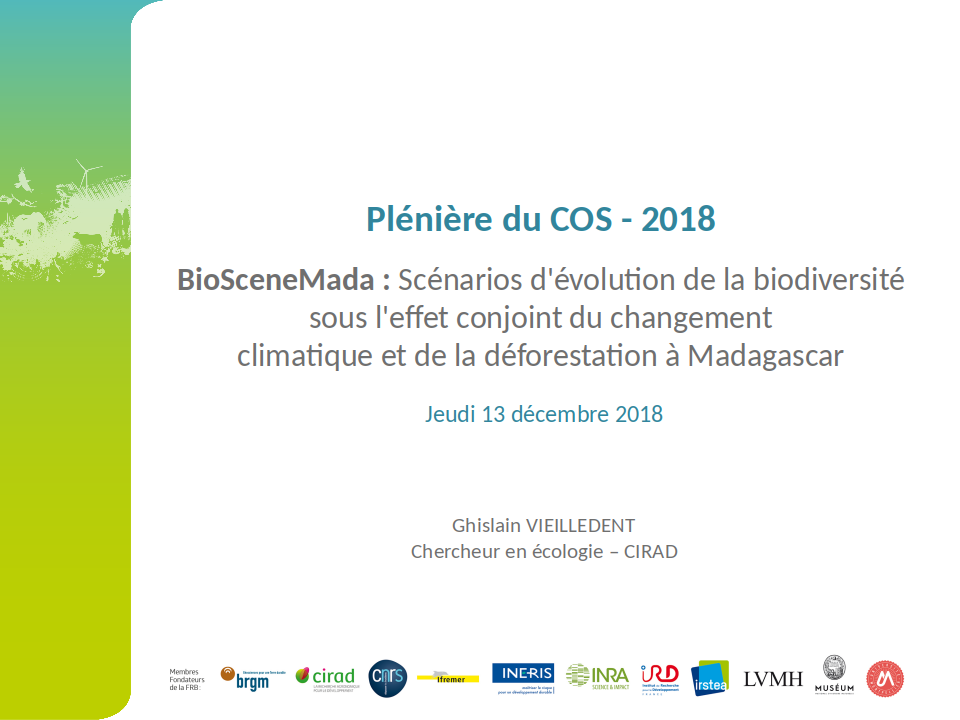
\includegraphics[height=\paperheight,width=\paperwidth]{figs/Masque.png}
%   }
%   \setbeamertemplate{navigation symbols}{}
%   % Remove shadow from block
%   \setbeamertemplate{blocks}[rounded][shadow=false]
%   \begin{frame}[plain]
%   \end{frame}
% }

% Title page
{
  \setbeamertemplate{navigation symbols}{}
  \begin{frame}[plain, noframenumbering]
  \begin{center}
  \small{\textbf{MELANOBS workshop -- Noumea, April 2024}}
  \end{center}
  \vspace{-0.5cm}
  \titlepage % Presentation first page
  \vspace{-3cm}
  \begin{center}
    
\includegraphics[width=\textwidth]{figs/Barre_couleur}
    
    \vspace{0.25cm}
    
    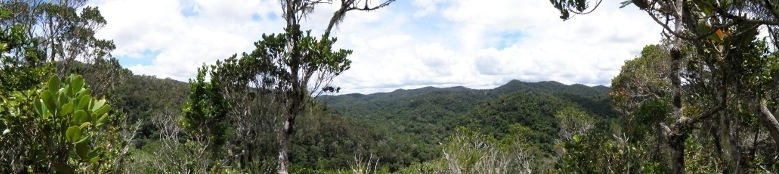
\includegraphics[width=10cm]{figs/Banniere}
    
    \small{Ghislain VIEILLEDENT$^{1, 2}$\hspace{0.25cm}Christelle VANCUTSEM$^{2}$\hspace{0.25cm}Frédéric ACHARD$^{2}$}
      
    \vspace{0.25cm}
    
    {\scriptsize
      \begin{tabular}{l}
        $[1]$ \textbf{Cirad} UMR AMAP, $[2]$ \textbf{EC JRC} Bioeconomy unit
      \end{tabular}
    }
    
    
\includegraphics[width=0.8\textwidth]{figs/partners_logos}
    
  \end{center}
  \end{frame}
}

% %%%%%%%%%%%%%%%%%%%%%%%%%%%%%%%%%%%%%%%%%%%%%%%%%%%%%%%%%%%%%%%%

\placelogotrue
\begin{frame}
  \frametitle{Plan}
  \begin{columns}[c]
    \begin{column}{0.5\textwidth}
      \tableofcontents[sections=1]
      \vspace{0.5cm}
      \tableofcontents[sections=2]
    \end{column}
    \begin{column}{0.5\textwidth}
        \tableofcontents[sections=3]
        \vspace{0.5cm}
        \tableofcontents[sections=4]
    \end{column}
  \end{columns}
\end{frame}
\placelogofalse

\section{Introduction}
\label{sec:orge4c2c94}
\subsection{Context}
\label{sec:org636b61b}
\begin{frame}[label={sec:orgedfa5a5}]{Tropical deforestation}
\centering 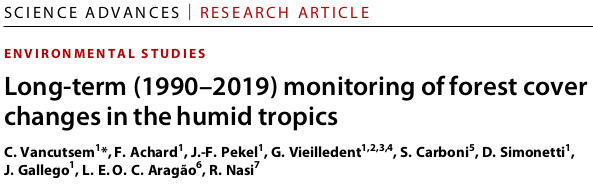
\includegraphics[width=8cm]{figs/Vancutsem2021}

\textbf{Vancutsem et al.} 2021, \emph{Science Advances}, doi:\href{https//doi.org10.1126/sciadv.abe1603}{10.1126/sciadv.abe1603}

\begin{itemize}
\item Tropical Moist Forest (TMF)
\item 1990--2019: Annual deforestation, degradation, regeneration
\end{itemize}
\end{frame}

\begin{frame}[label={sec:org97f6835}]{Tropical deforestation}
\begin{itemize}
\item Full Landsat archive (1982--2019), 30m pixel, time-series analysis
\item Classification tree based on expert knowledge
\item Tropical deforestation was underestimated (-33\% in 2000--2012, Hansen
et al. 2013)
\item Maps and data: \url{https://forobs.jrc.ec.europa.eu/TMF/}
\end{itemize}

\vspace{0.25cm}
\centering 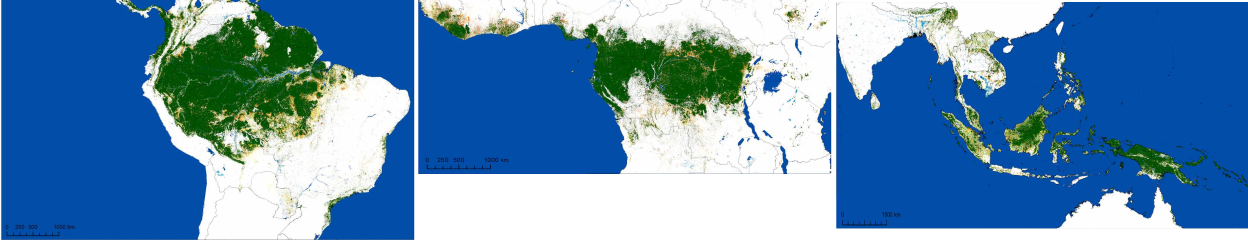
\includegraphics[width=\textwidth]{figs/Vancutsem2021-maps-wide}
\end{frame}

\begin{frame}[label={sec:orgbbf4ebb}]{Tropical deforestation}
\begin{itemize}
\item Precise enough to visually identify the causes of deforestation
(logging, fires, agriculture)
\end{itemize}

\centering 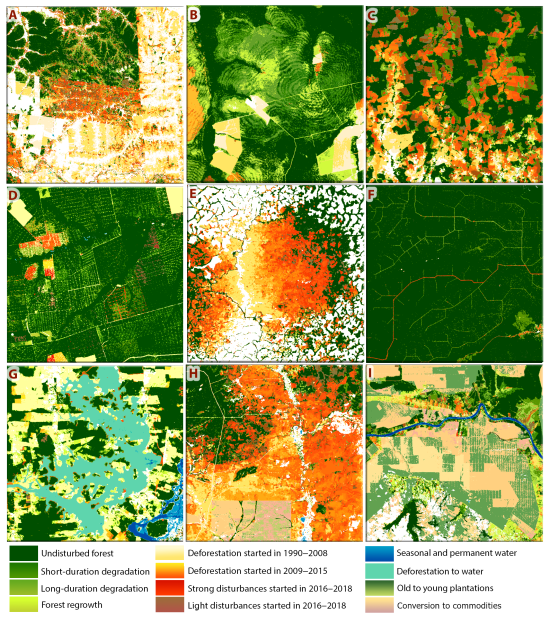
\includegraphics[height=0.7\textheight]{figs/Vancutsem2021-patterns}
\end{frame}

\subsection{Objectives}
\label{sec:org32a5111}
\begin{frame}[label={sec:orgd62c374}]{Forecasting deforestation}
\begin{itemize}
\item About 7 Mha of tropical moist forest are disappearing each year (size
of Ireland)
\item At this rate, will tropical forests still exist in 2100?
\item If yes, where will they be located?
\item What will be the consequences of future deforestation on biodiversity
and carbon emissions?
\end{itemize}

\vspace{0.5cm}
\centering 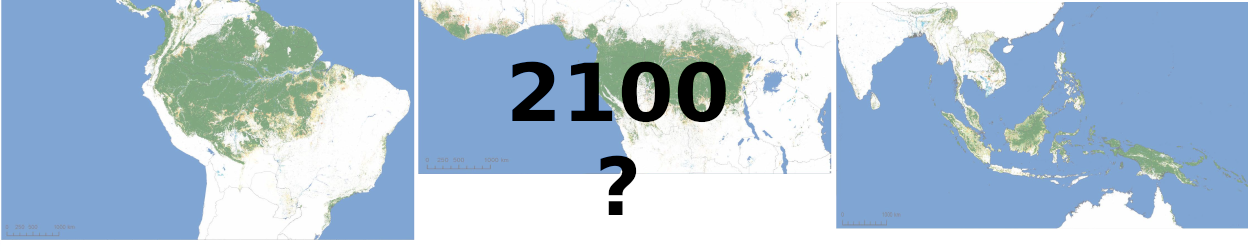
\includegraphics[width=\textwidth]{figs/Vancutsem2021-maps-2100}
\end{frame}

\begin{frame}[label={sec:org64bf647}]{Forecasting deforestation}
Why is it a timely question?

\begin{itemize}
\item \textbf{Alert} decision makers
\item Carbon emissions scenarios (\(\rightarrow\) IPCC)
\item Biodiversity scenarios (\(\rightarrow\) IPBES)
\item Local scale: systematic conservation planning (protected area network,
REDD\(+\))
\item Modelling \(\rightarrow\) main spatial drivers of deforestation
\end{itemize}

\vspace{0.10cm}
\centering 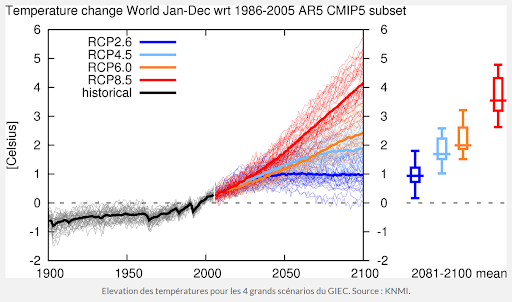
\includegraphics[width=0.55\textwidth]{figs/ipcc.png}\\[0pt]
\textbf{IPCC scenarios}
\end{frame}

\begin{frame}[label={sec:org41602ef}]{Forecasting deforestation \textbf{spatially}}
Why is \textbf{spatial} forecasting important?

Because both biodiversity and carbon stocks vary strongly in space.

\vspace{0.25cm}

\begin{tabular}{cc}
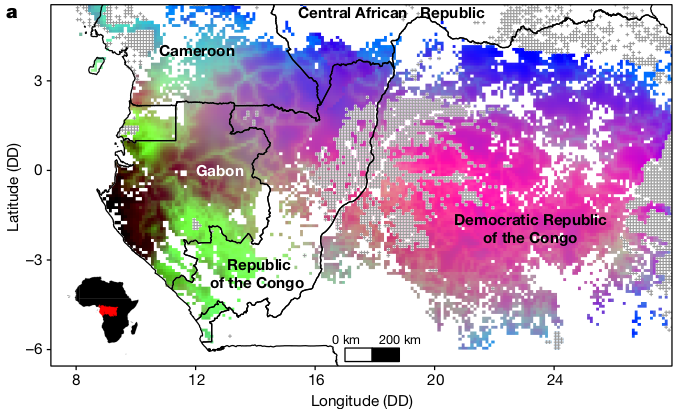
\includegraphics[width=0.5\textwidth]{figs/Rejou2021-Floristic} & 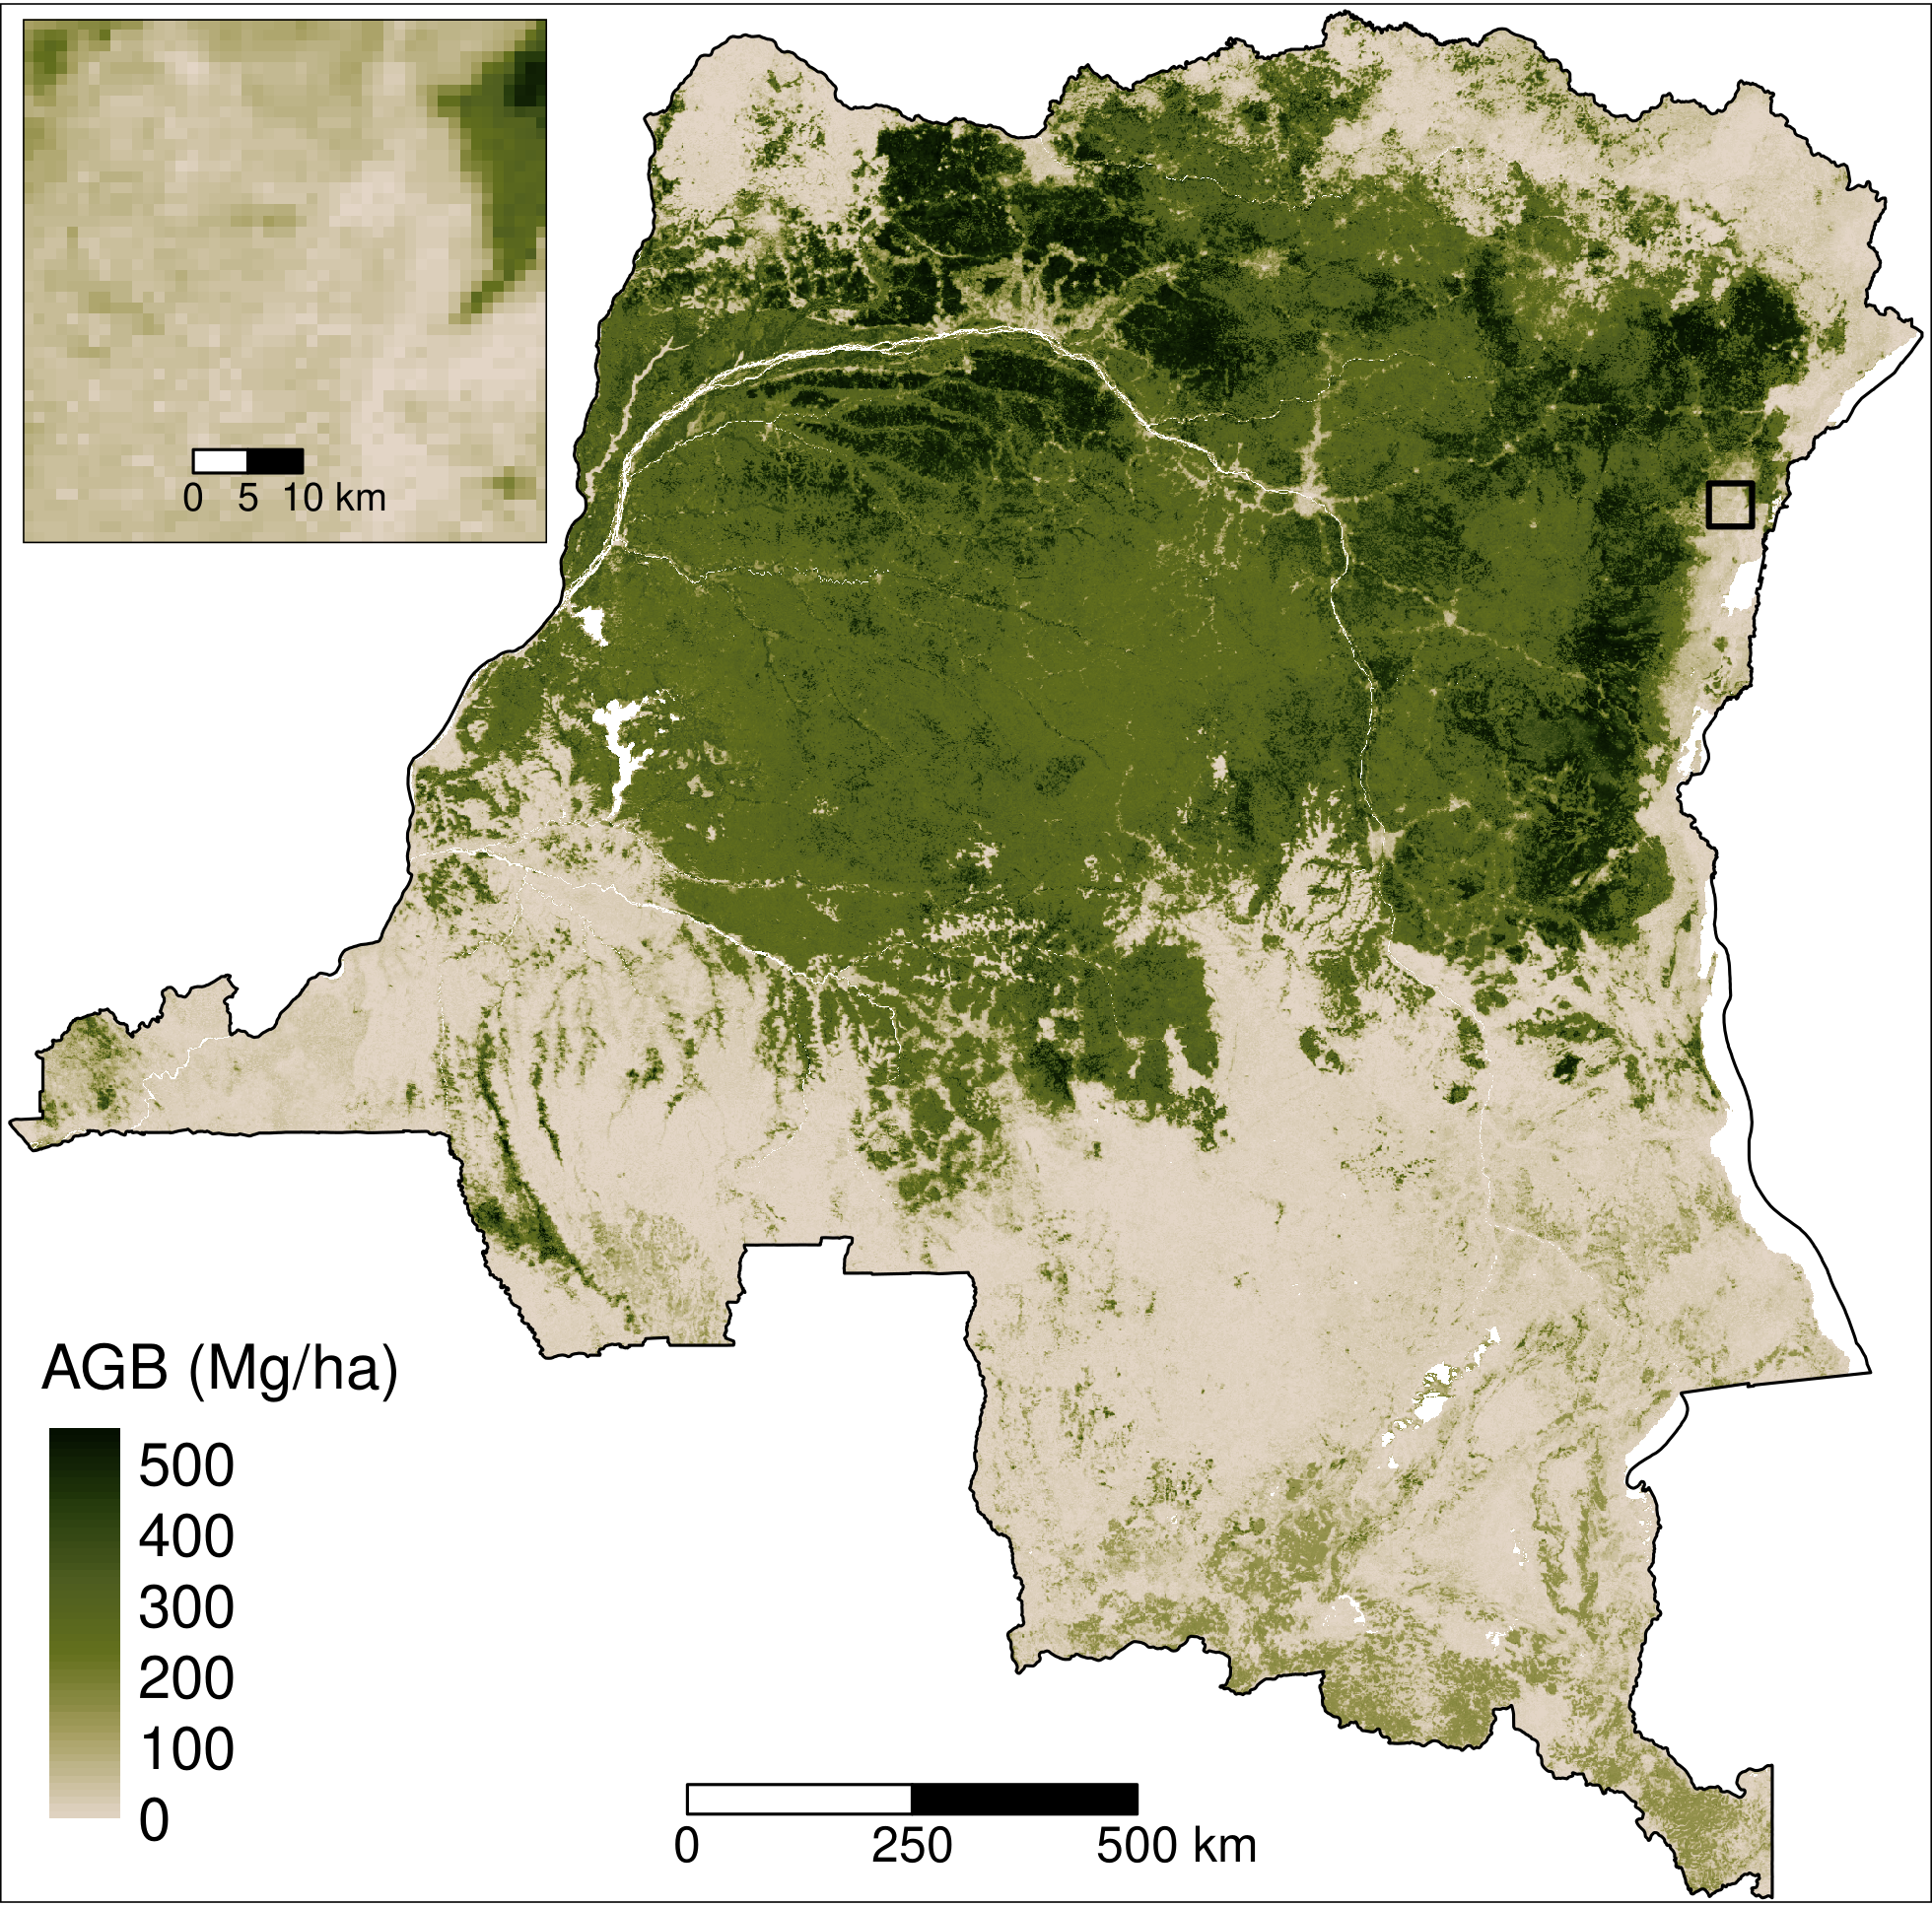
\includegraphics[width=0.40\textwidth]{figs/sm/AGB}\\
\textbf{Community map} & \textbf{AGB map in DRC} \\
(Réjou-Méchain 2021) & ~
\end{tabular}
\end{frame}

\subsection{Approach}
\label{sec:org1242cc3}
\begin{frame}[label={sec:org51856ad}]{Approach}
\begin{itemize}
\item \textbf{i.} Consider tropical moist forest in \textbf{92} countries (119 study areas)
\item \textbf{ii.} Estimate the current deforestation rate and uncertainty in each country
\item \textbf{iii.} Model the spatial risk of deforestation from environmental factors
\item \textbf{iv.} Forecast the deforestation assuming a business-as-usual scenario
\item \textbf{v.} Consequences in terms of biodiversity and carbon emissions
\end{itemize}

\vspace{0.5cm}
\begin{center}
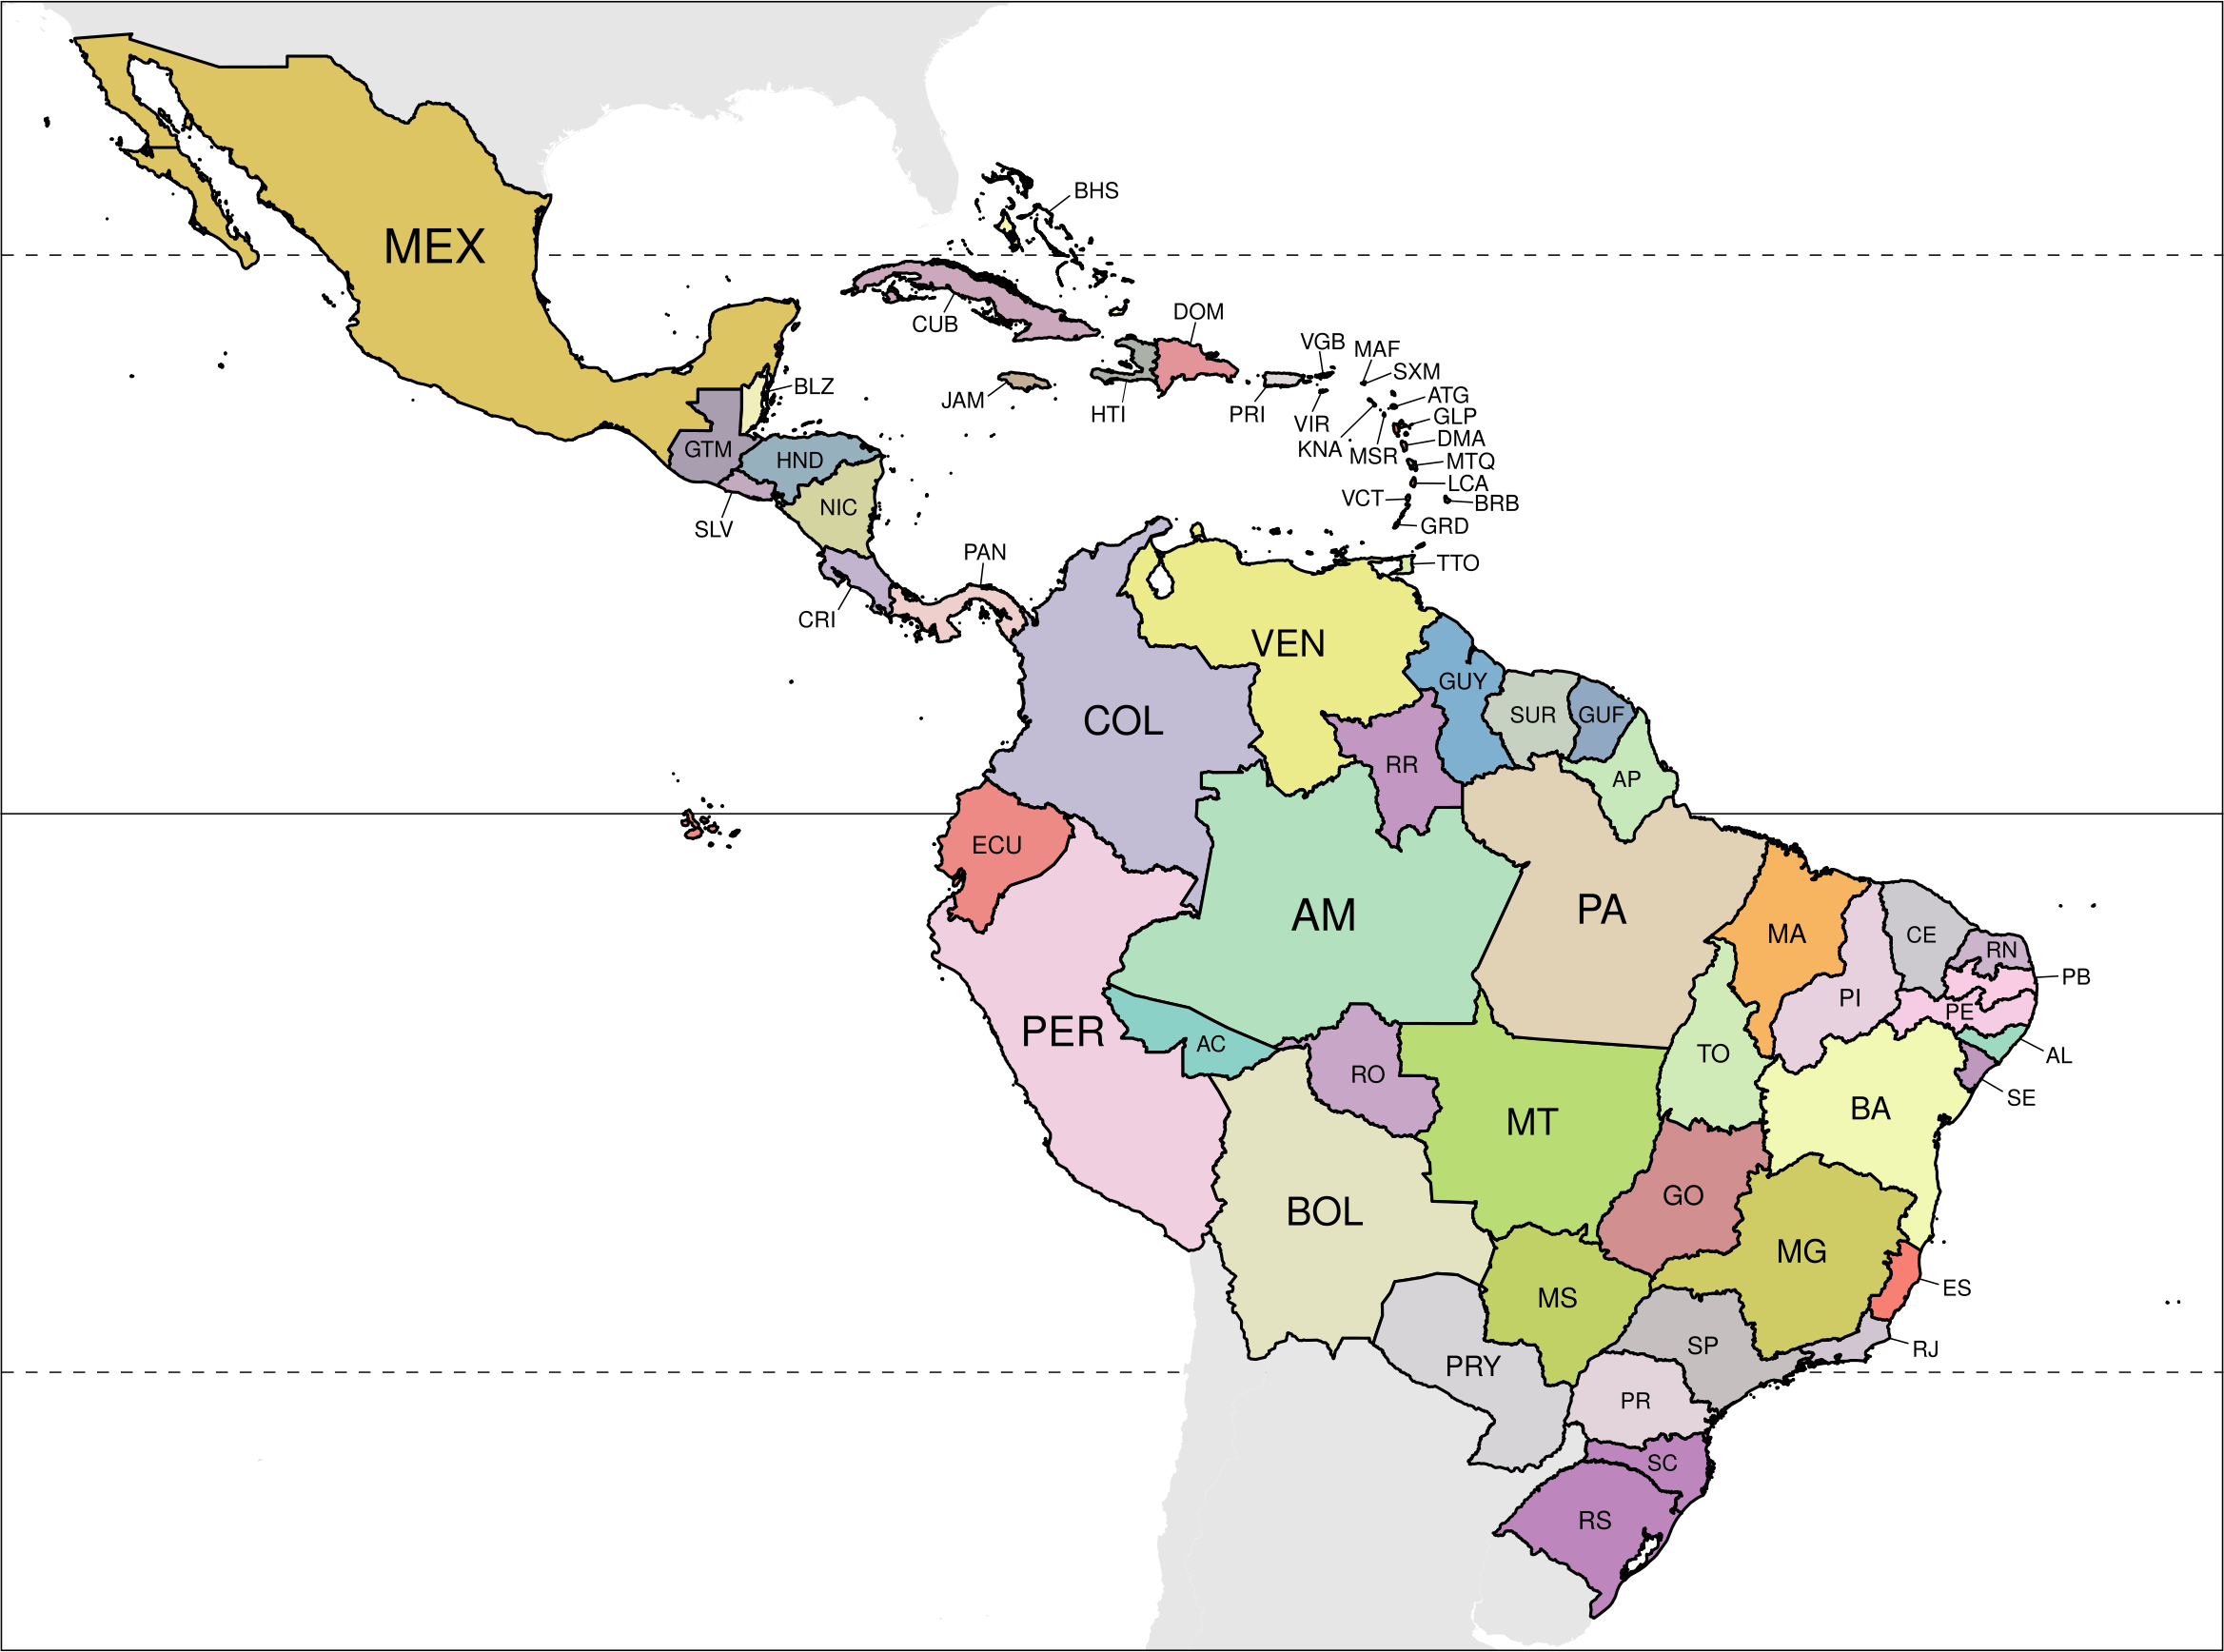
\includegraphics[width=0.32\textwidth]{figs/sm/study_areas_America}
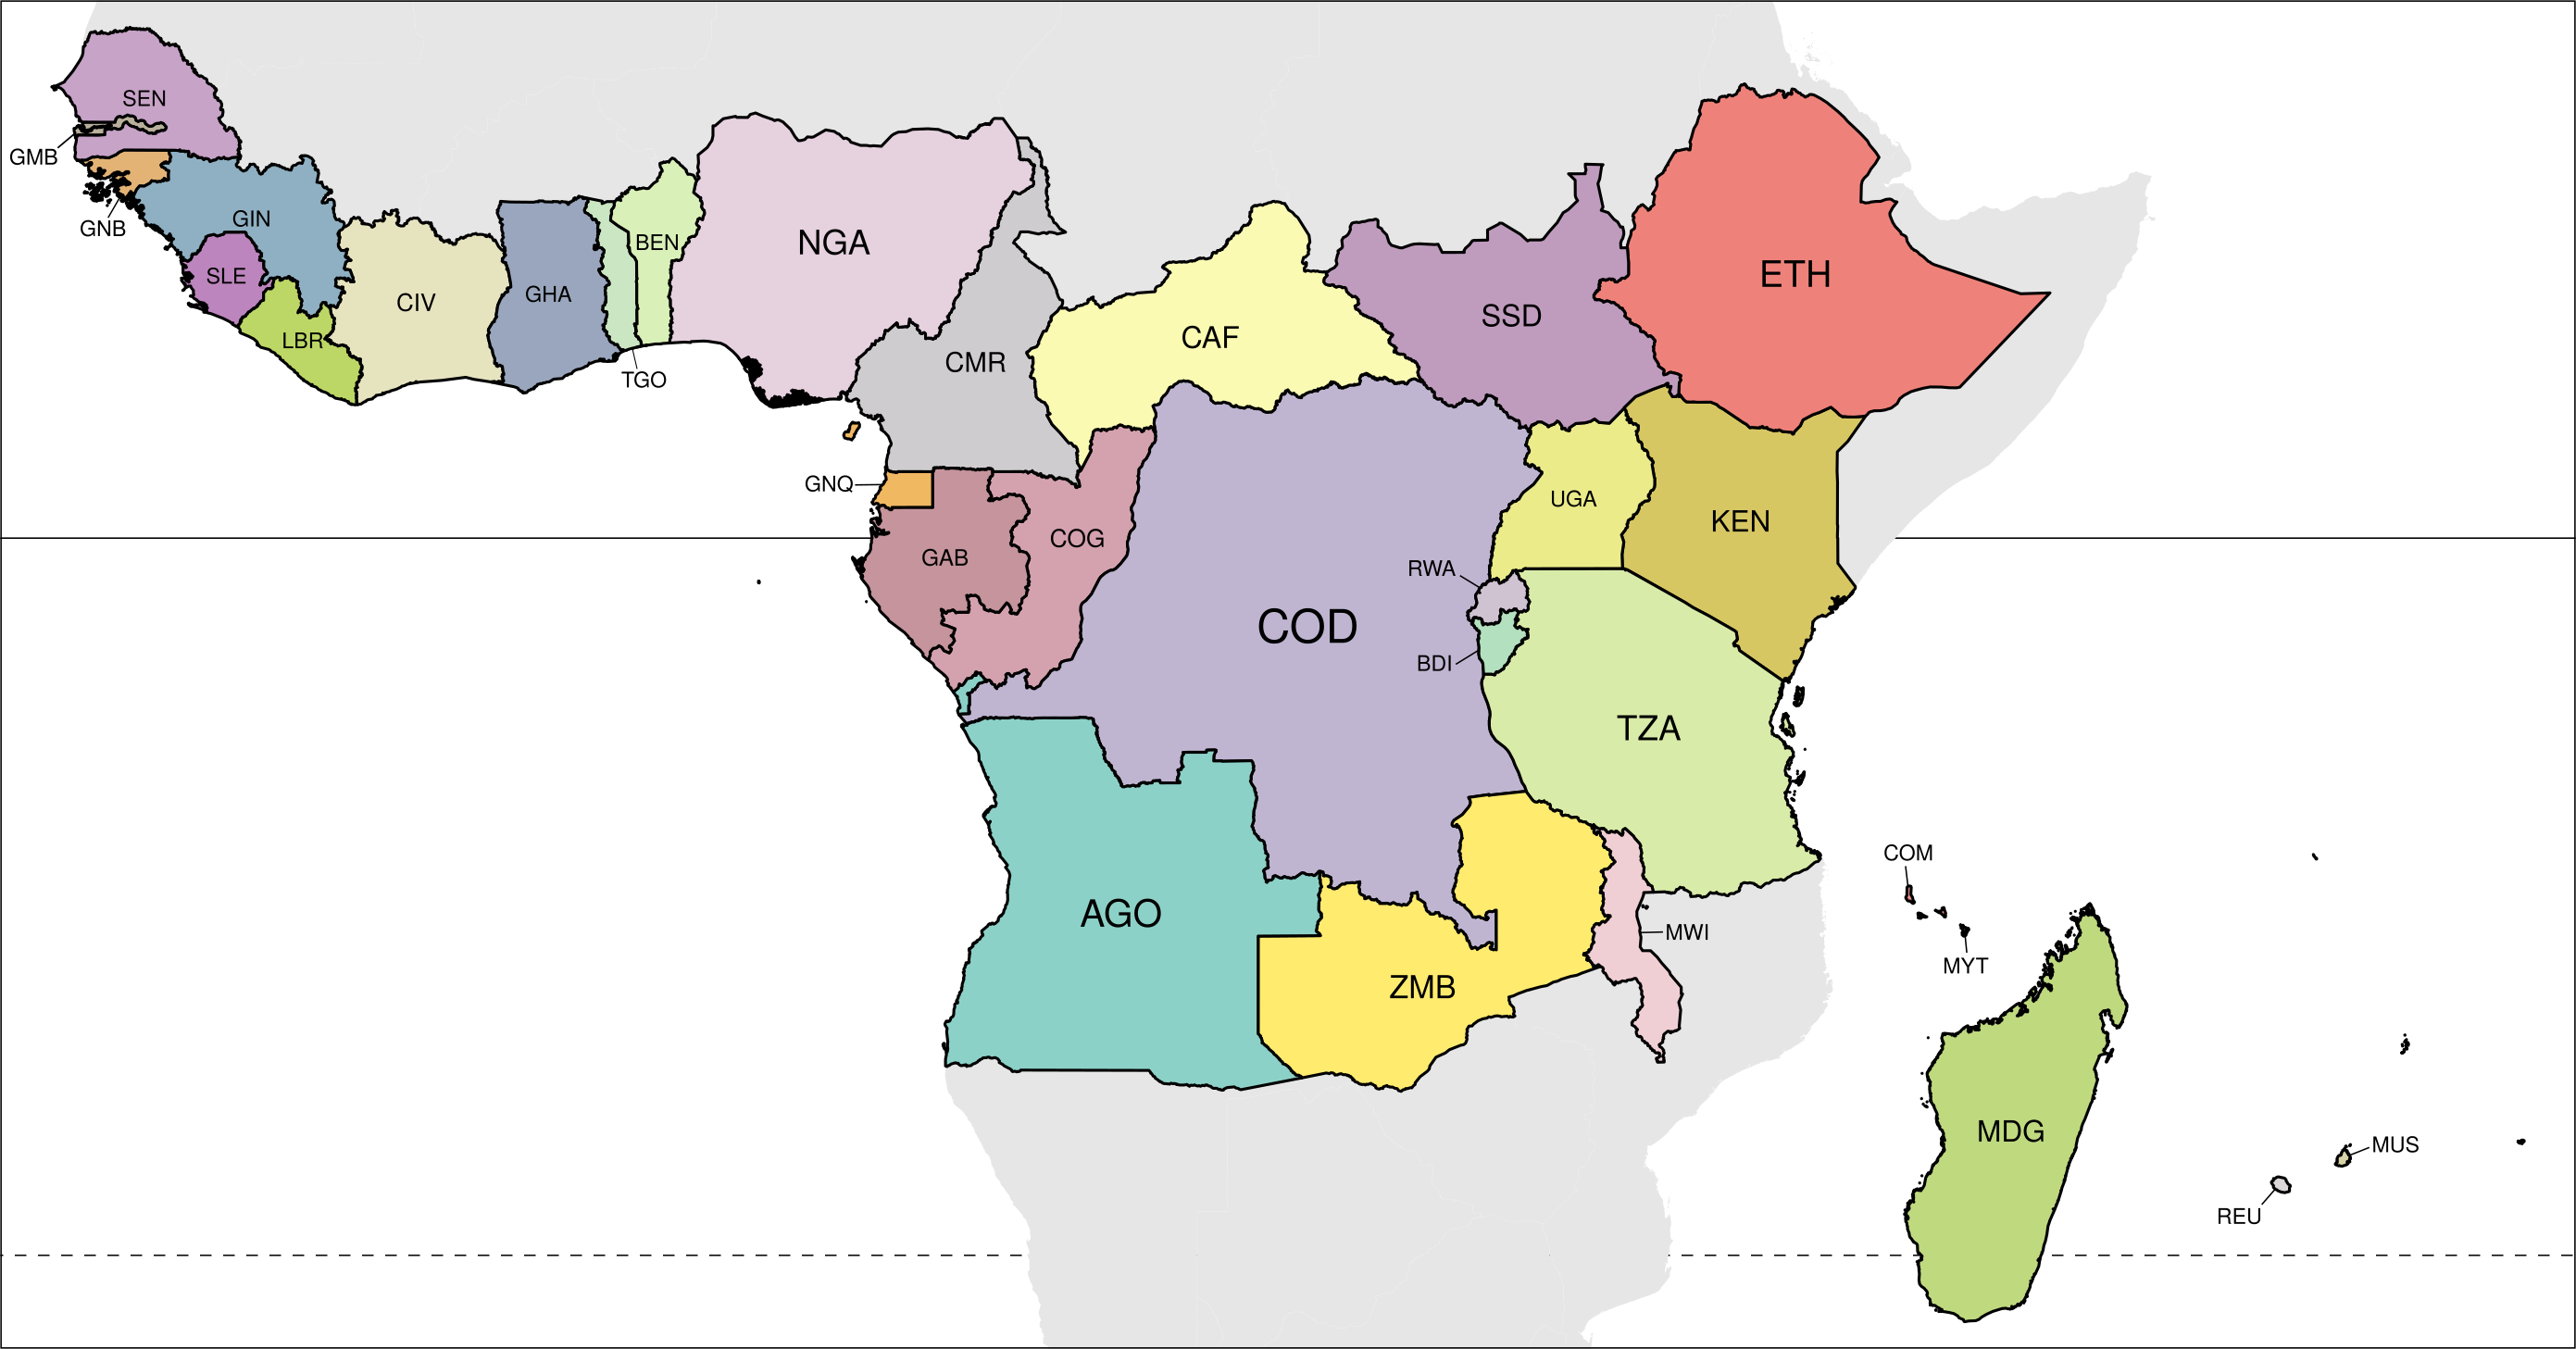
\includegraphics[width=0.32\textwidth]{figs/sm/study_areas_Africa}
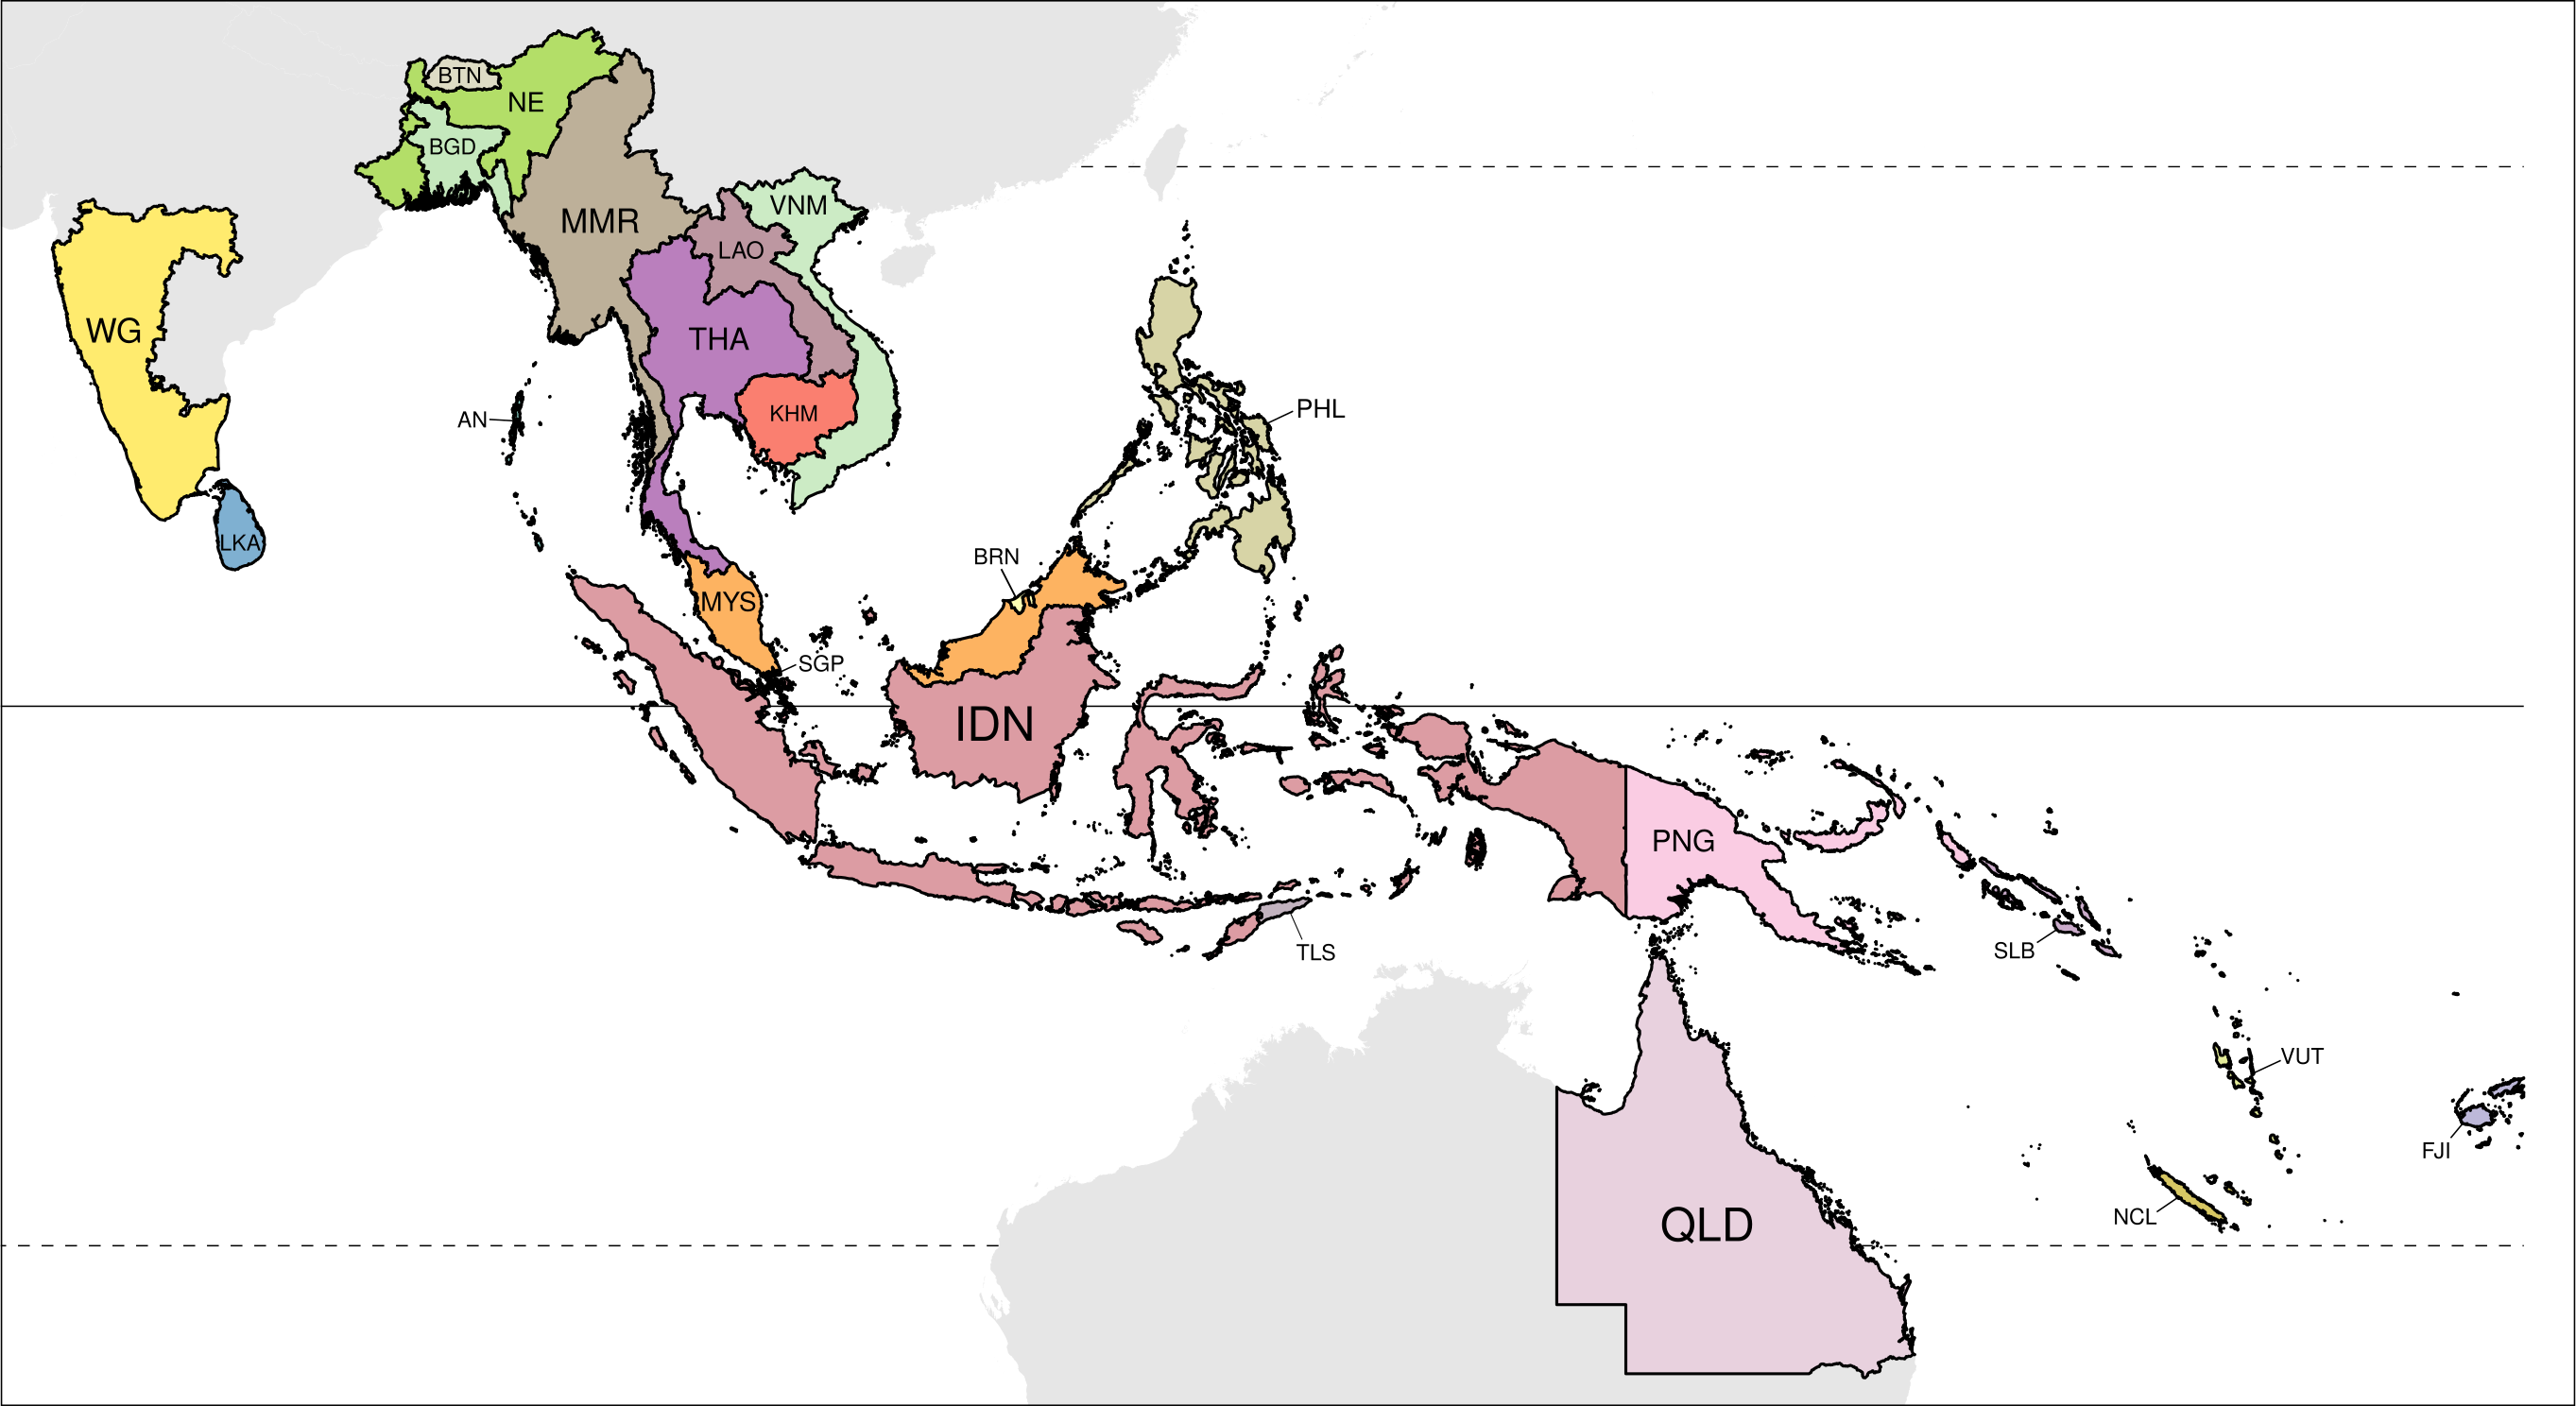
\includegraphics[width=0.32\textwidth]{figs/sm/study_areas_Asia}
\textbf{The 119 study areas in the 3 continents}
\end{center}
\end{frame}

\section{Methods}
\label{sec:orge5dcb9a}
\subsection{Models}
\label{sec:orgeff6c1d}
\begin{frame}[label={sec:orgdcccb81}]{Modelling the intensity of deforestation}
\begin{columns}
\begin{column}{0.5\columnwidth}
\begin{itemize}
\item 10 values of annual deforested area (ha/yr) in 2010--2020 per country
\item (Brazil: per state, India: per region)
\item Mean deforestation rate (ha/yr) in 2010--2020 per country
\item Uncertainty around the mean (95\% confidence interval)
\end{itemize}
\end{column}

\begin{column}{0.5\columnwidth}
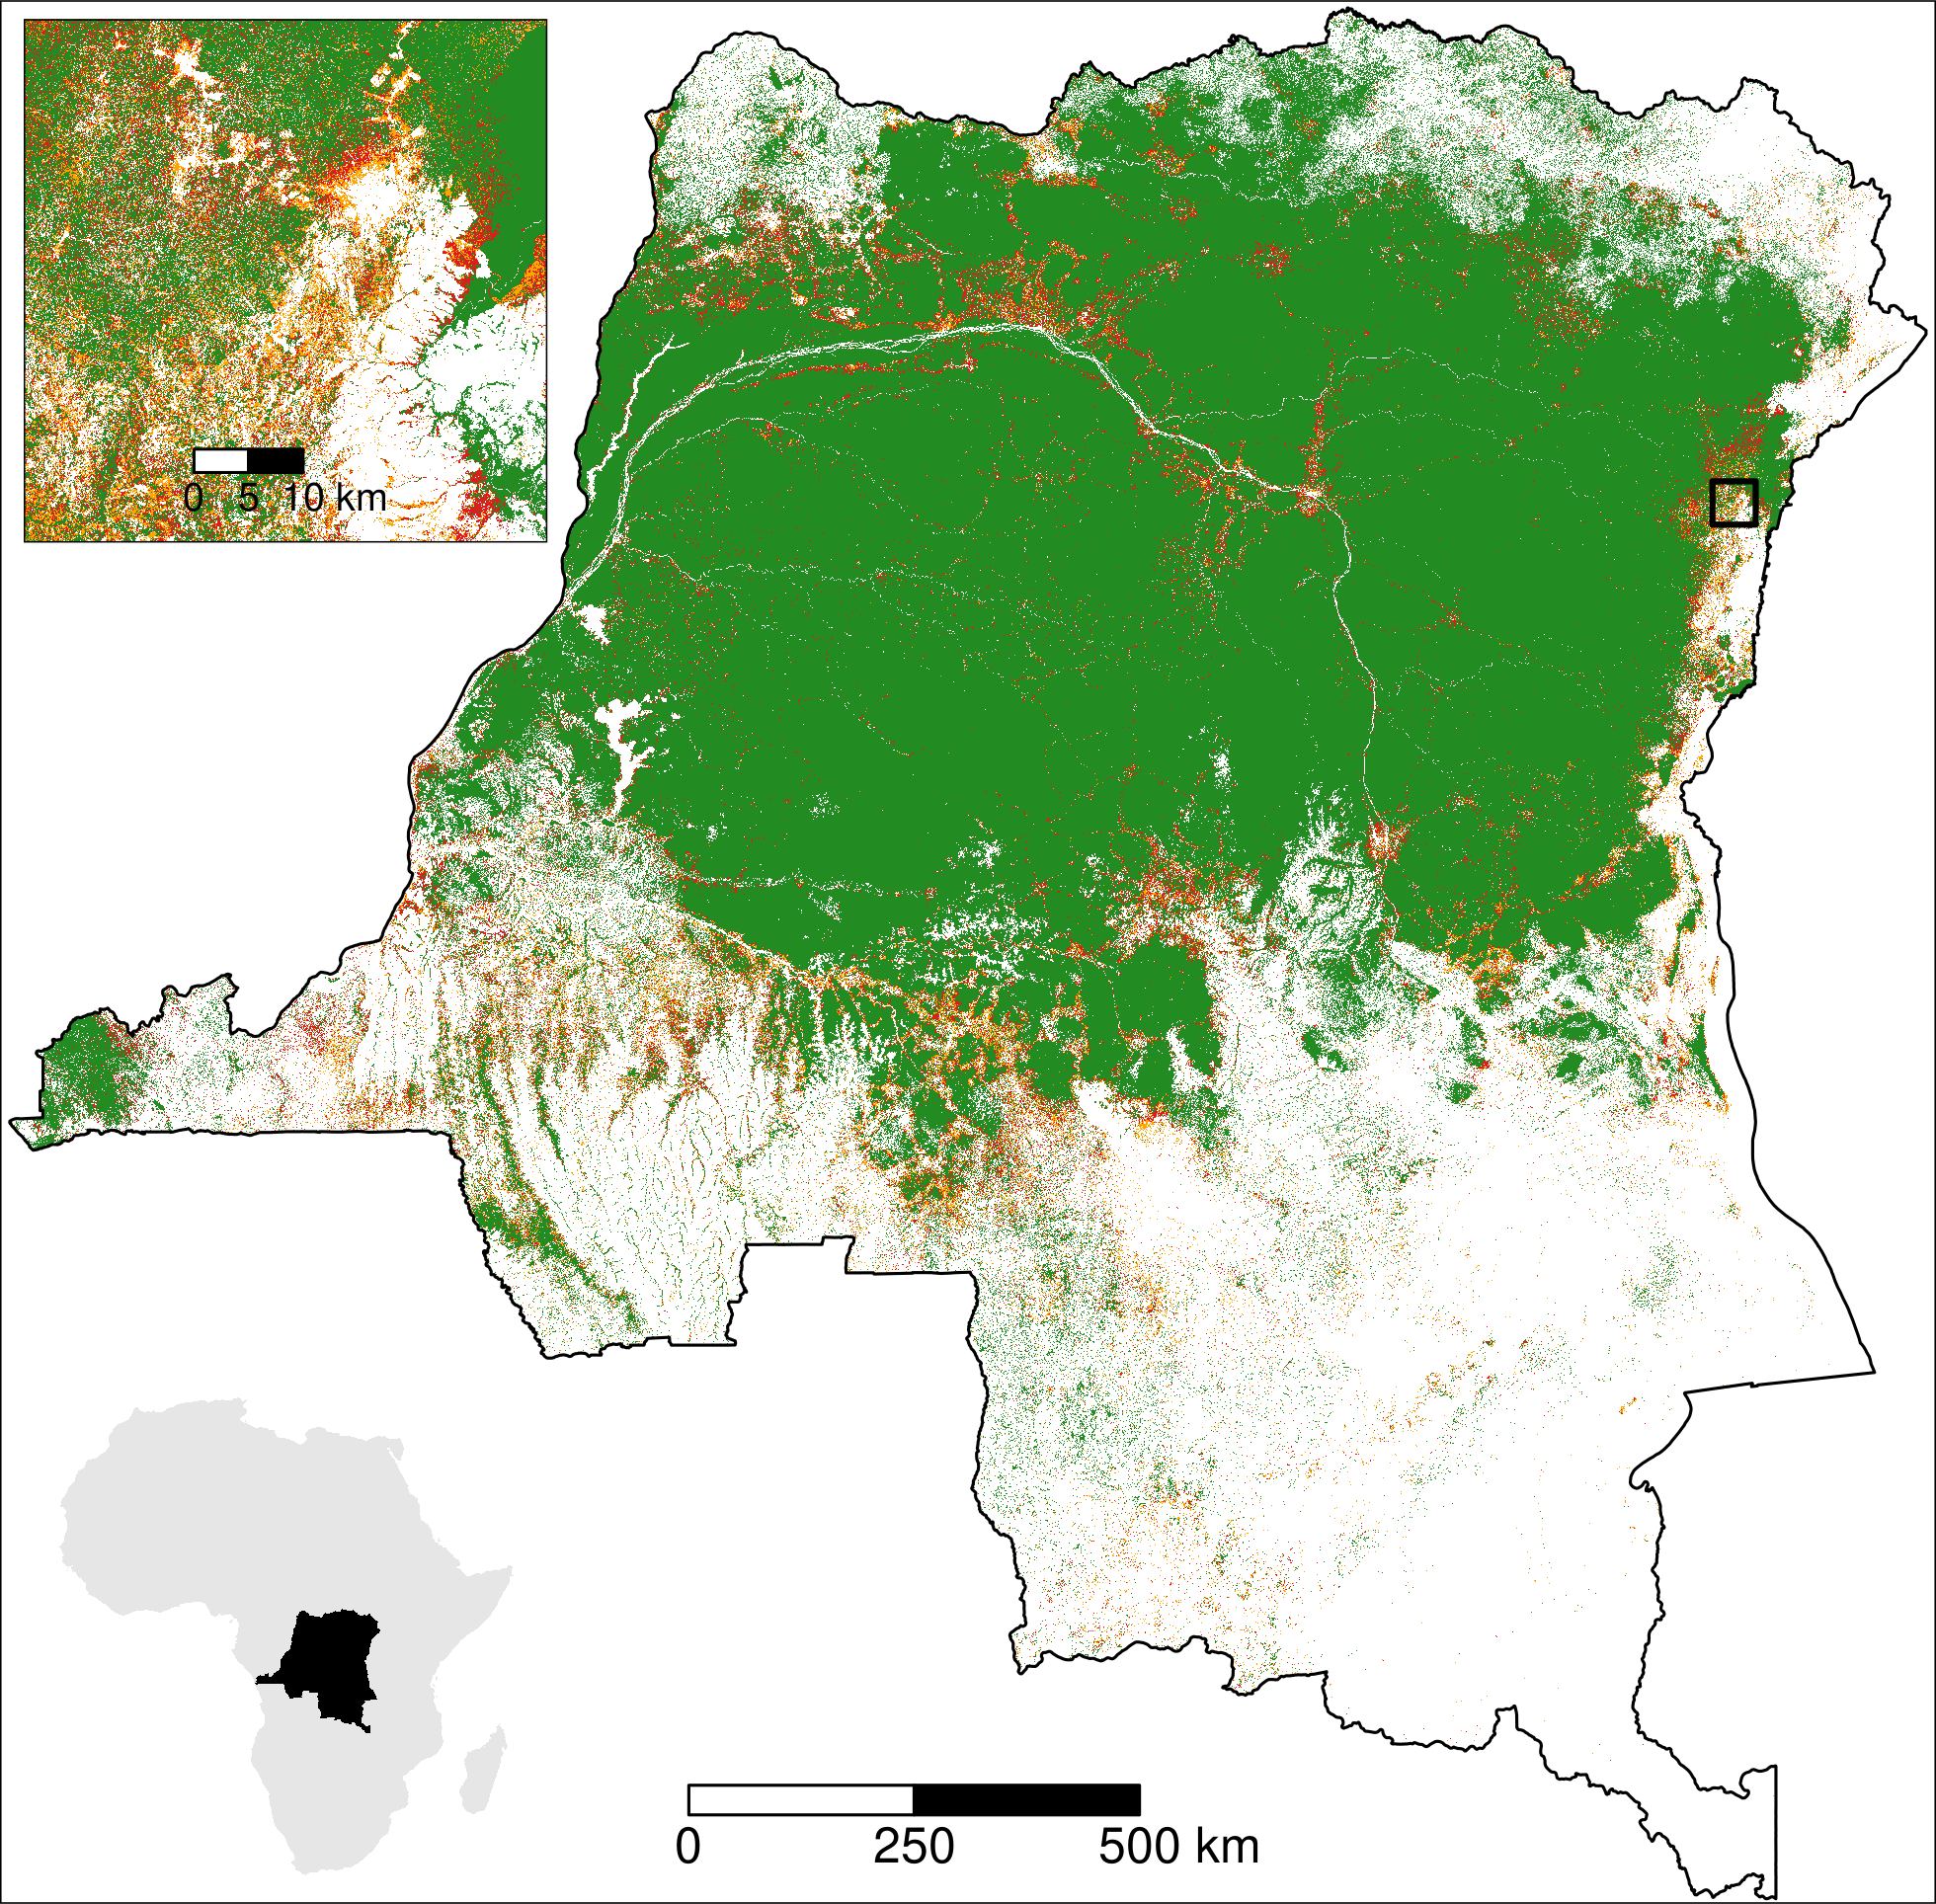
\includegraphics[width=\textwidth]{figs/sm/fcc123}

\textbf{Past deforestation 2000--2010--2020 in DRC}
\end{column}
\end{columns}
\end{frame}

\begin{frame}[label={sec:org22b437c}]{Modelling the intensity of deforestation}
\centering 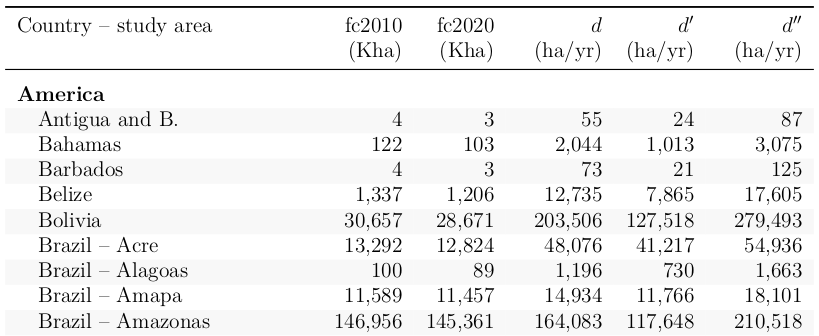
\includegraphics[width=0.8\textwidth]{figs/d_ci}

\textbf{Examples of mean deforestation rate with uncertainty}
\end{frame}

\begin{frame}[label={sec:orgda4c3f3}]{Modelling the spatial risk of deforestation}
\begin{columns}
\begin{column}{0.5\columnwidth}
A logistic regression model with iCAR process

\begin{equation*}
\begin{split}
  y_i \sim \mathcal{B}ernoulli(\theta_i)\\
  \text{logit}(\theta_i) = \alpha + X_i \beta + \rho_{j(i)}\\
  \rho_{j(i)} \sim \mathcal{N}ormal(\sum_{j^{\prime}} \rho_{j^{\prime}} / n_j,V_{\rho} / n_j)
\end{split}
\end{equation*}

\footnotesize (NB: We compared this model with a simple GLM and a Random
Forest model using a cross-validation procedure)
\end{column}

\begin{column}{0.5\columnwidth}
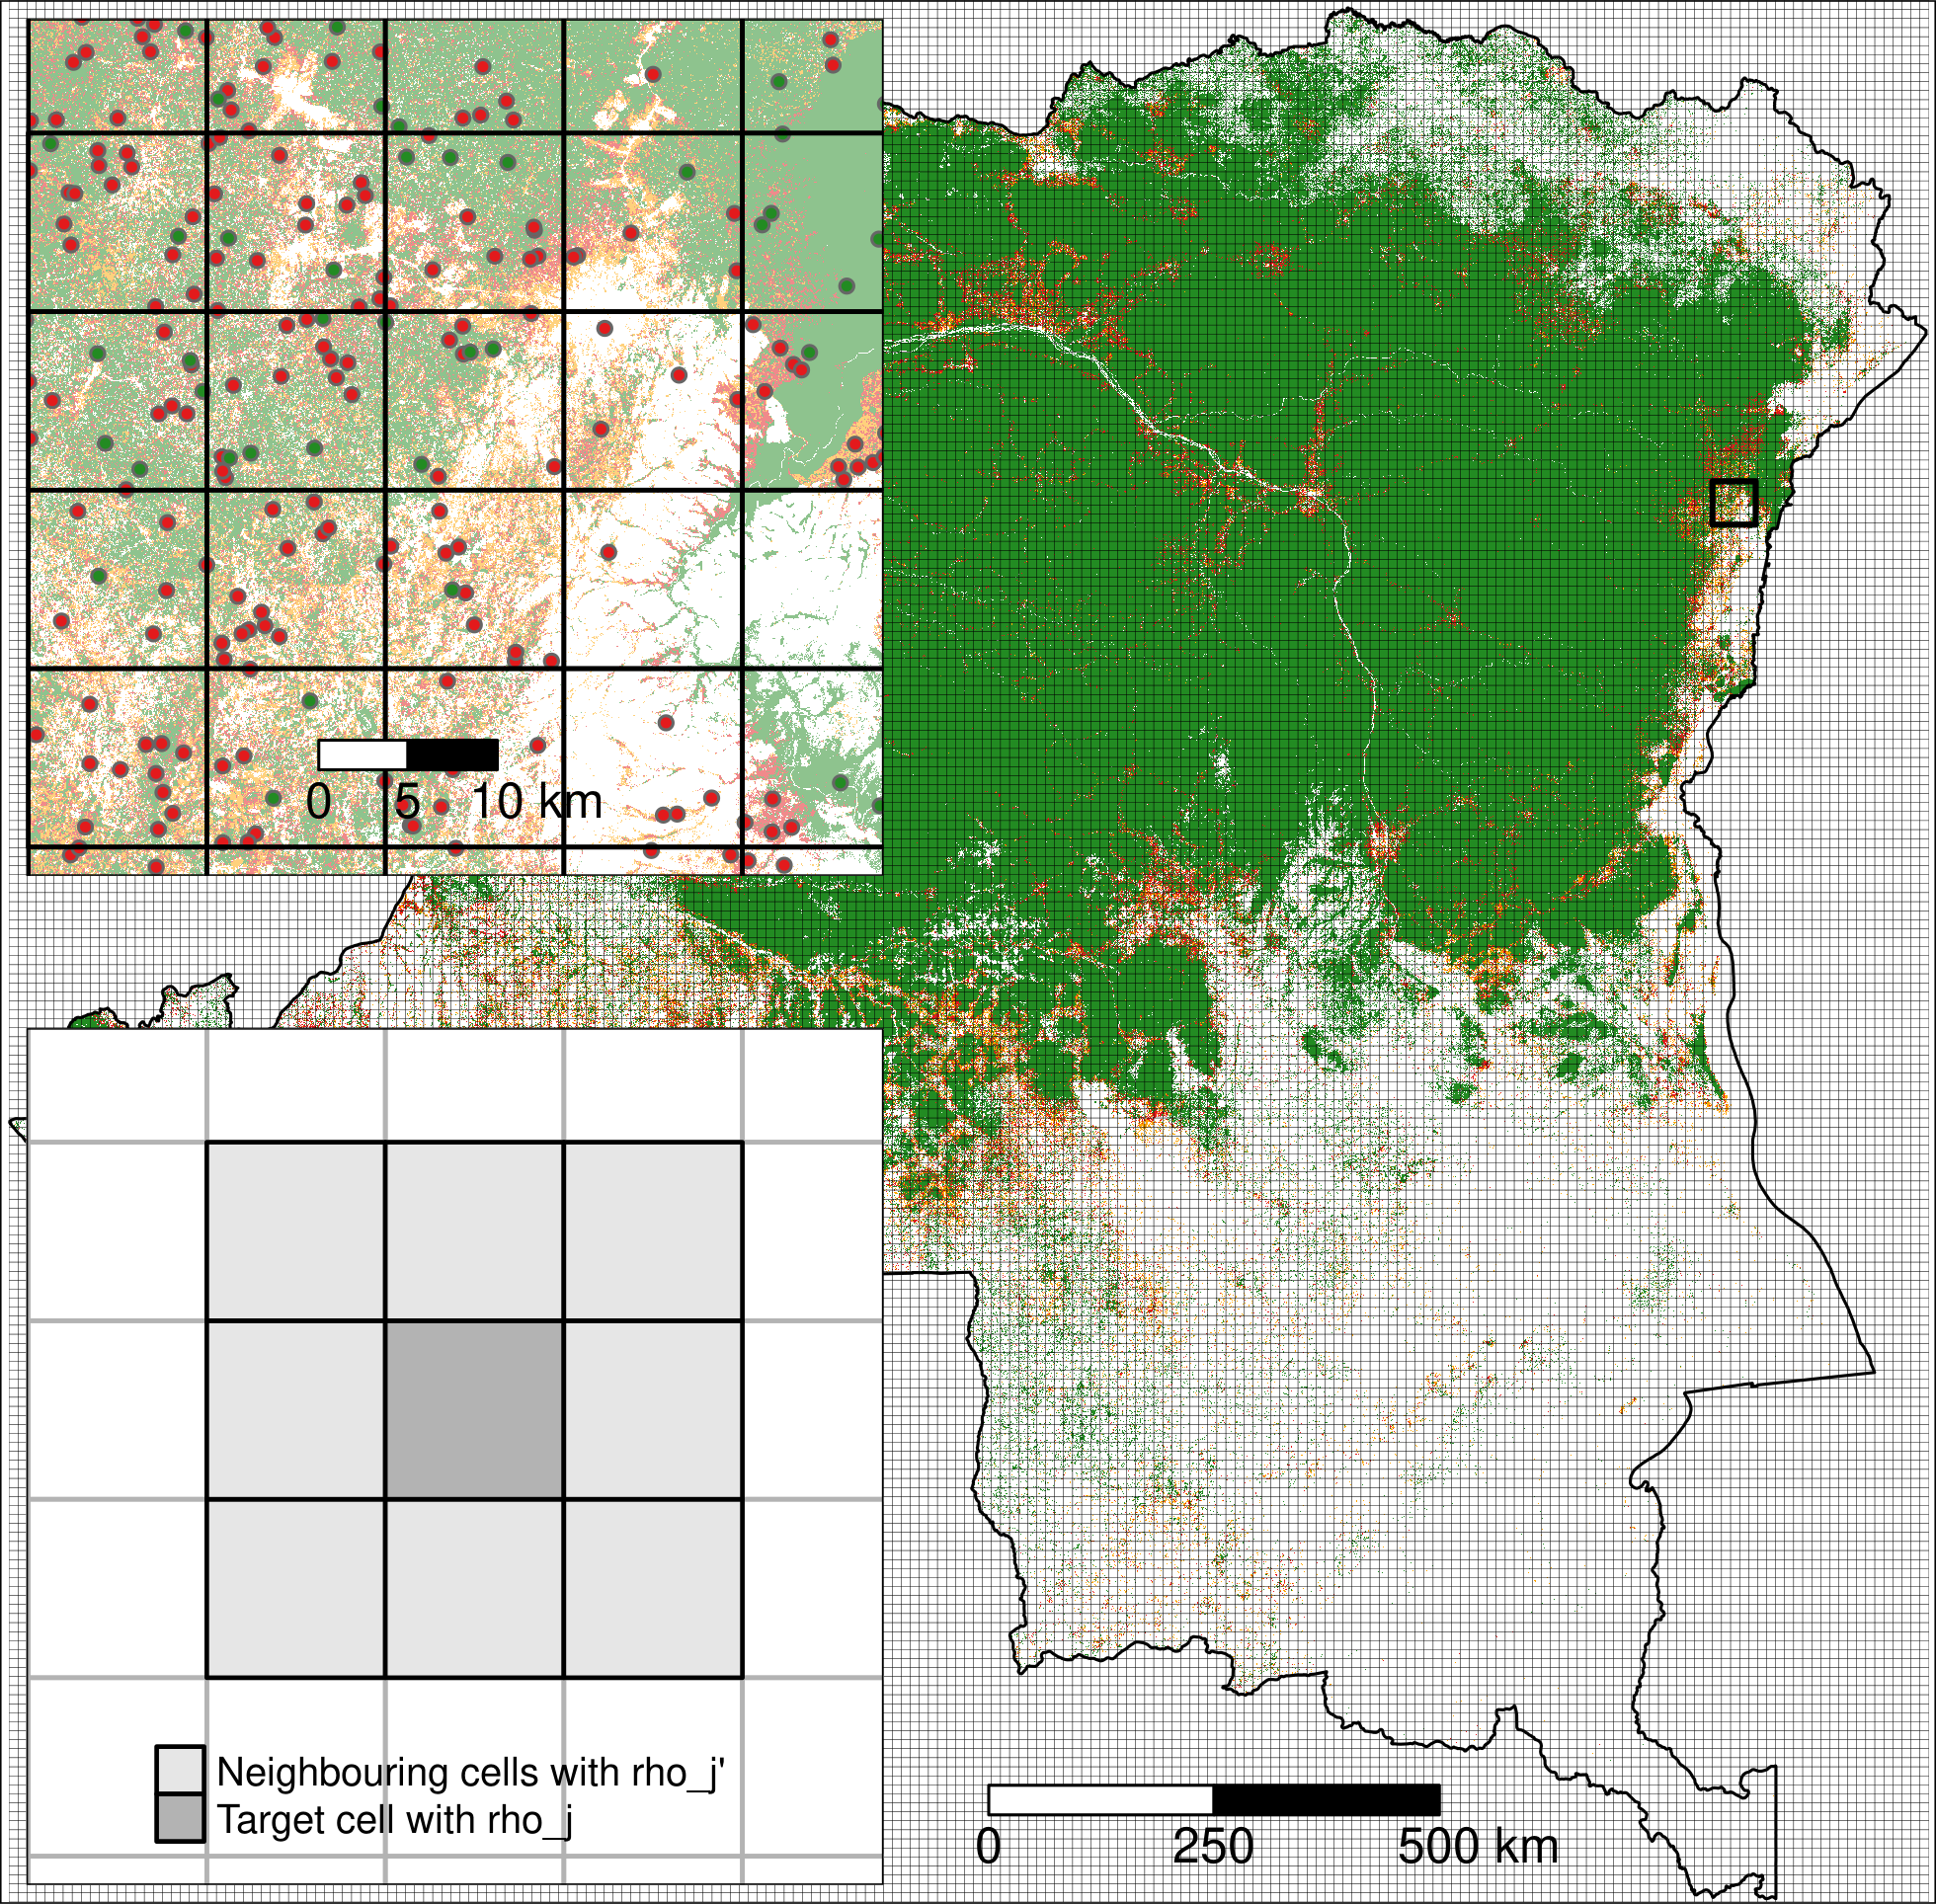
\includegraphics[width=\textwidth]{figs/sm/grid}

\textbf{Square grid of 10km cells over DRC}
\end{column}
\end{columns}
\end{frame}

\subsection{Spatial variables}
\label{sec:orgb082088}
\begin{frame}[label={sec:orgfaea2ed}]{Spatial variables}
\begin{itemize}
\item Height explanatory variables
\end{itemize}

\centering 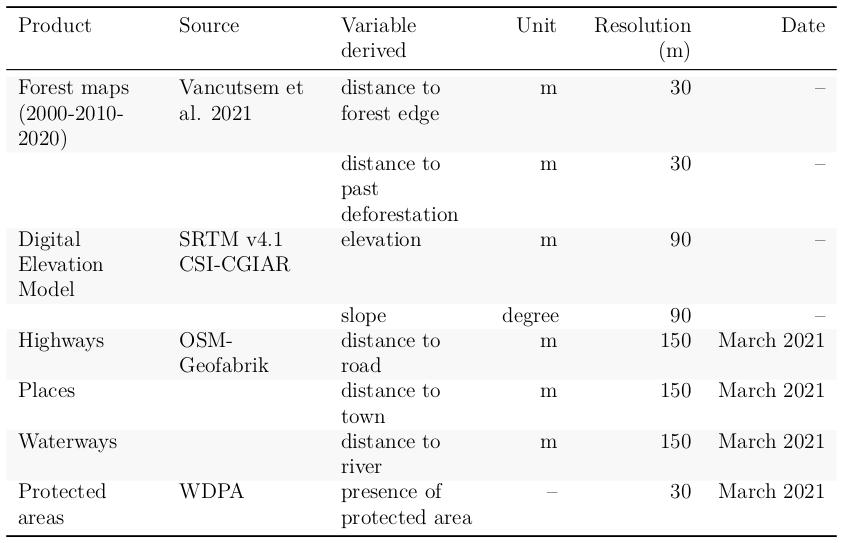
\includegraphics[width=0.7\textwidth]{figs/variables-tab}
\end{frame}

\begin{frame}[label={sec:org8f95bb8}]{Spatial variables}
\centering 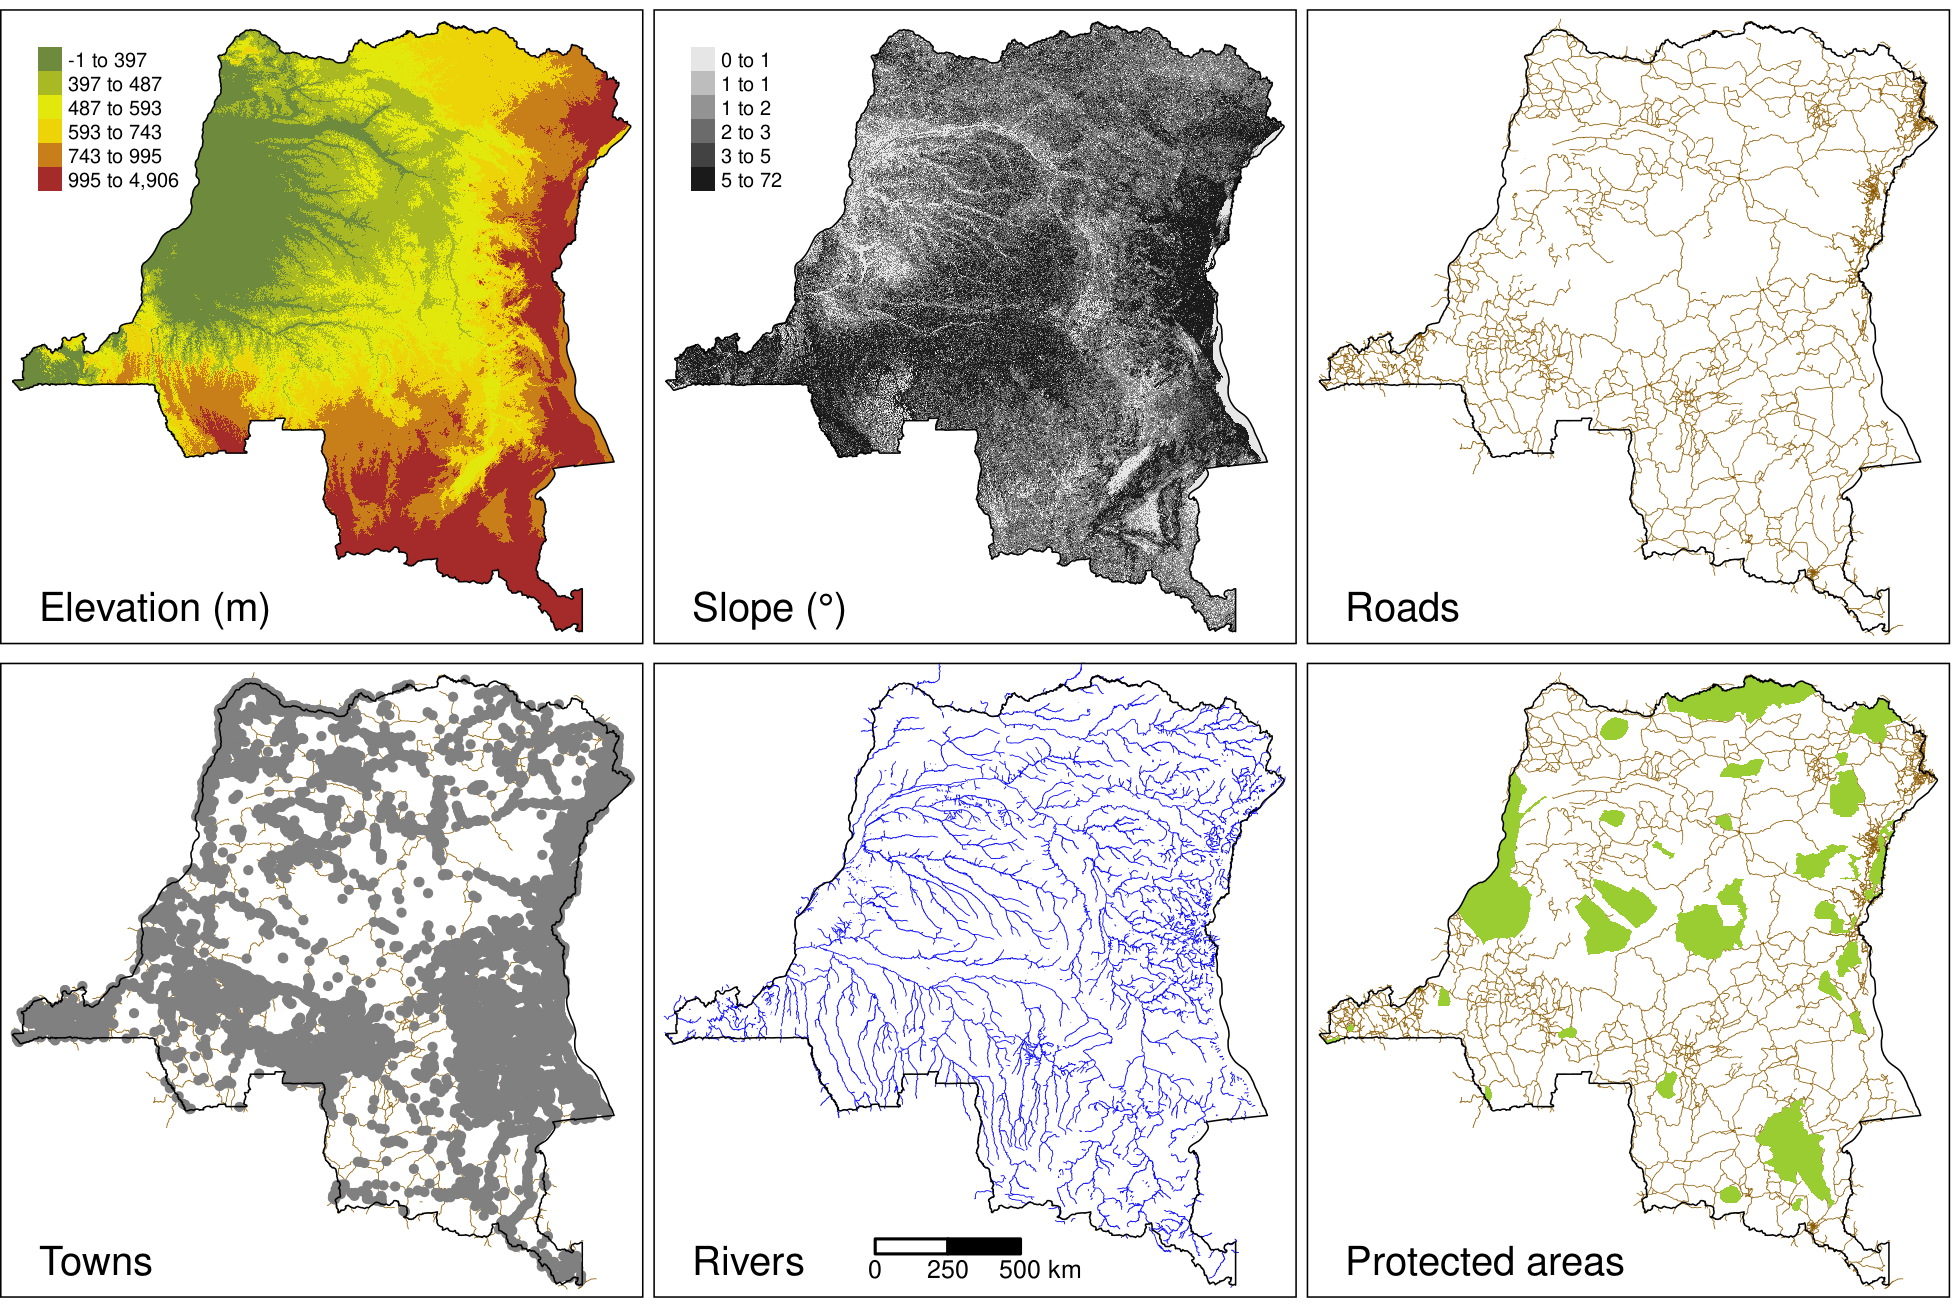
\includegraphics[width=0.8\textwidth]{figs/sm/var.png}

\textbf{Spatial explanatory variables in DRC}
\end{frame}

\begin{frame}[label={sec:org4e5ce09}]{Roads}
\begin{itemize}
\item OpenStreetMap (OSM)
\item ``motorway'', ``trunk'', ``primary'', ``secondary'' and ``tertiary'' roads
\item 3.6 million roads from OSM
\end{itemize}

\centering 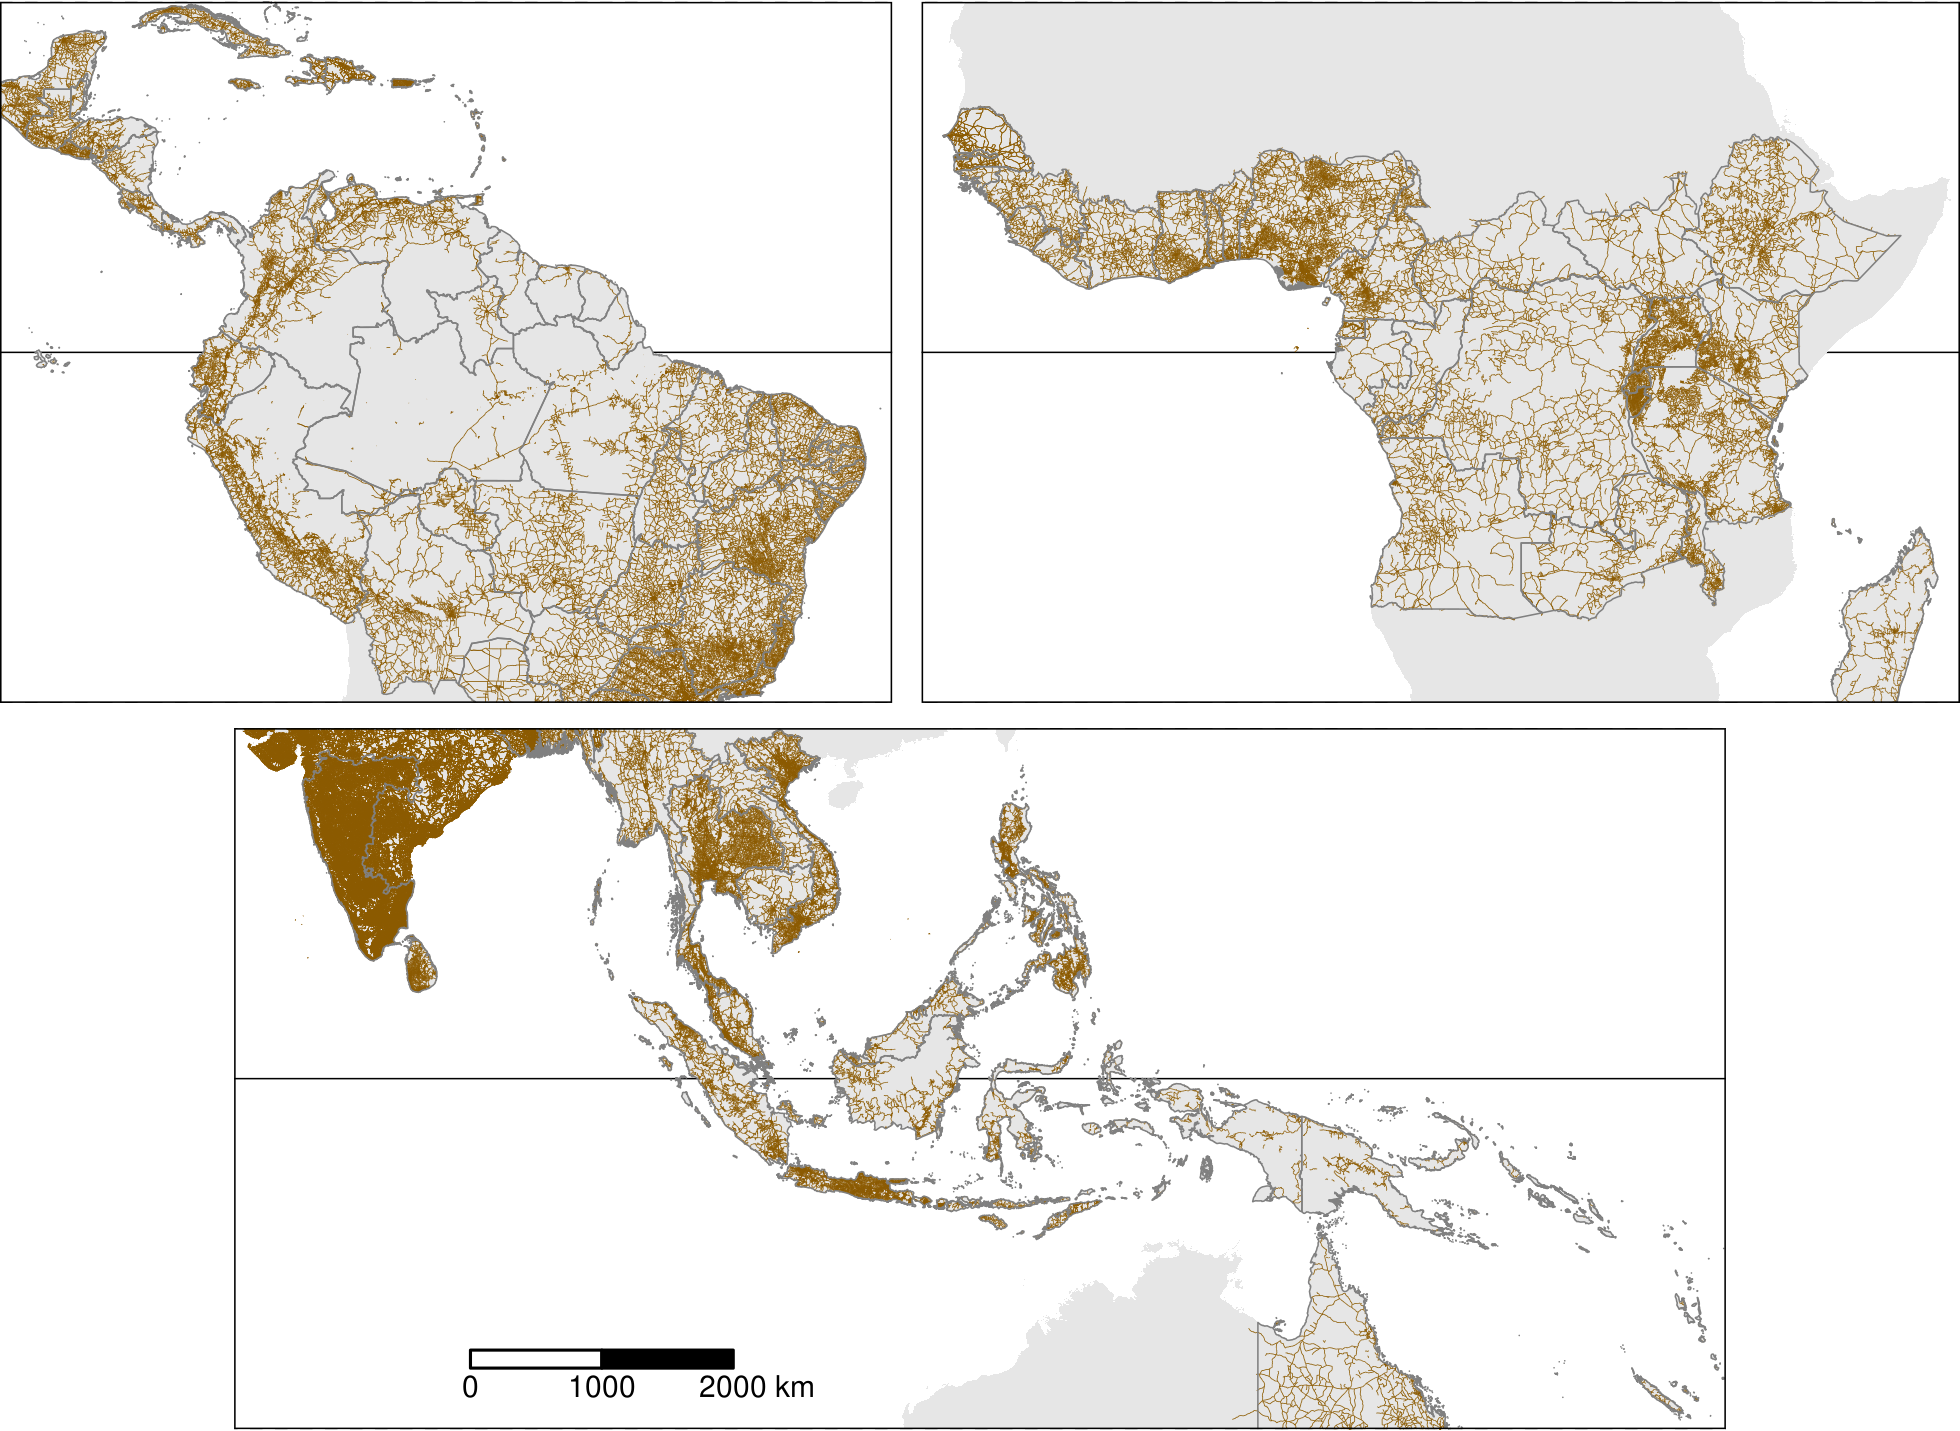
\includegraphics[width=0.7\textwidth]{figs/sm/roads.png}
\end{frame}

\begin{frame}[label={sec:org5184ae6}]{Protected areas}
\begin{itemize}
\item PA status: ``Designated'', ``Inscribed'', ``Established'', or ``Proposed''
before 1\textsuperscript{st} January 2010
\item 85,000 protected areas from WDPA
\end{itemize}

\centering 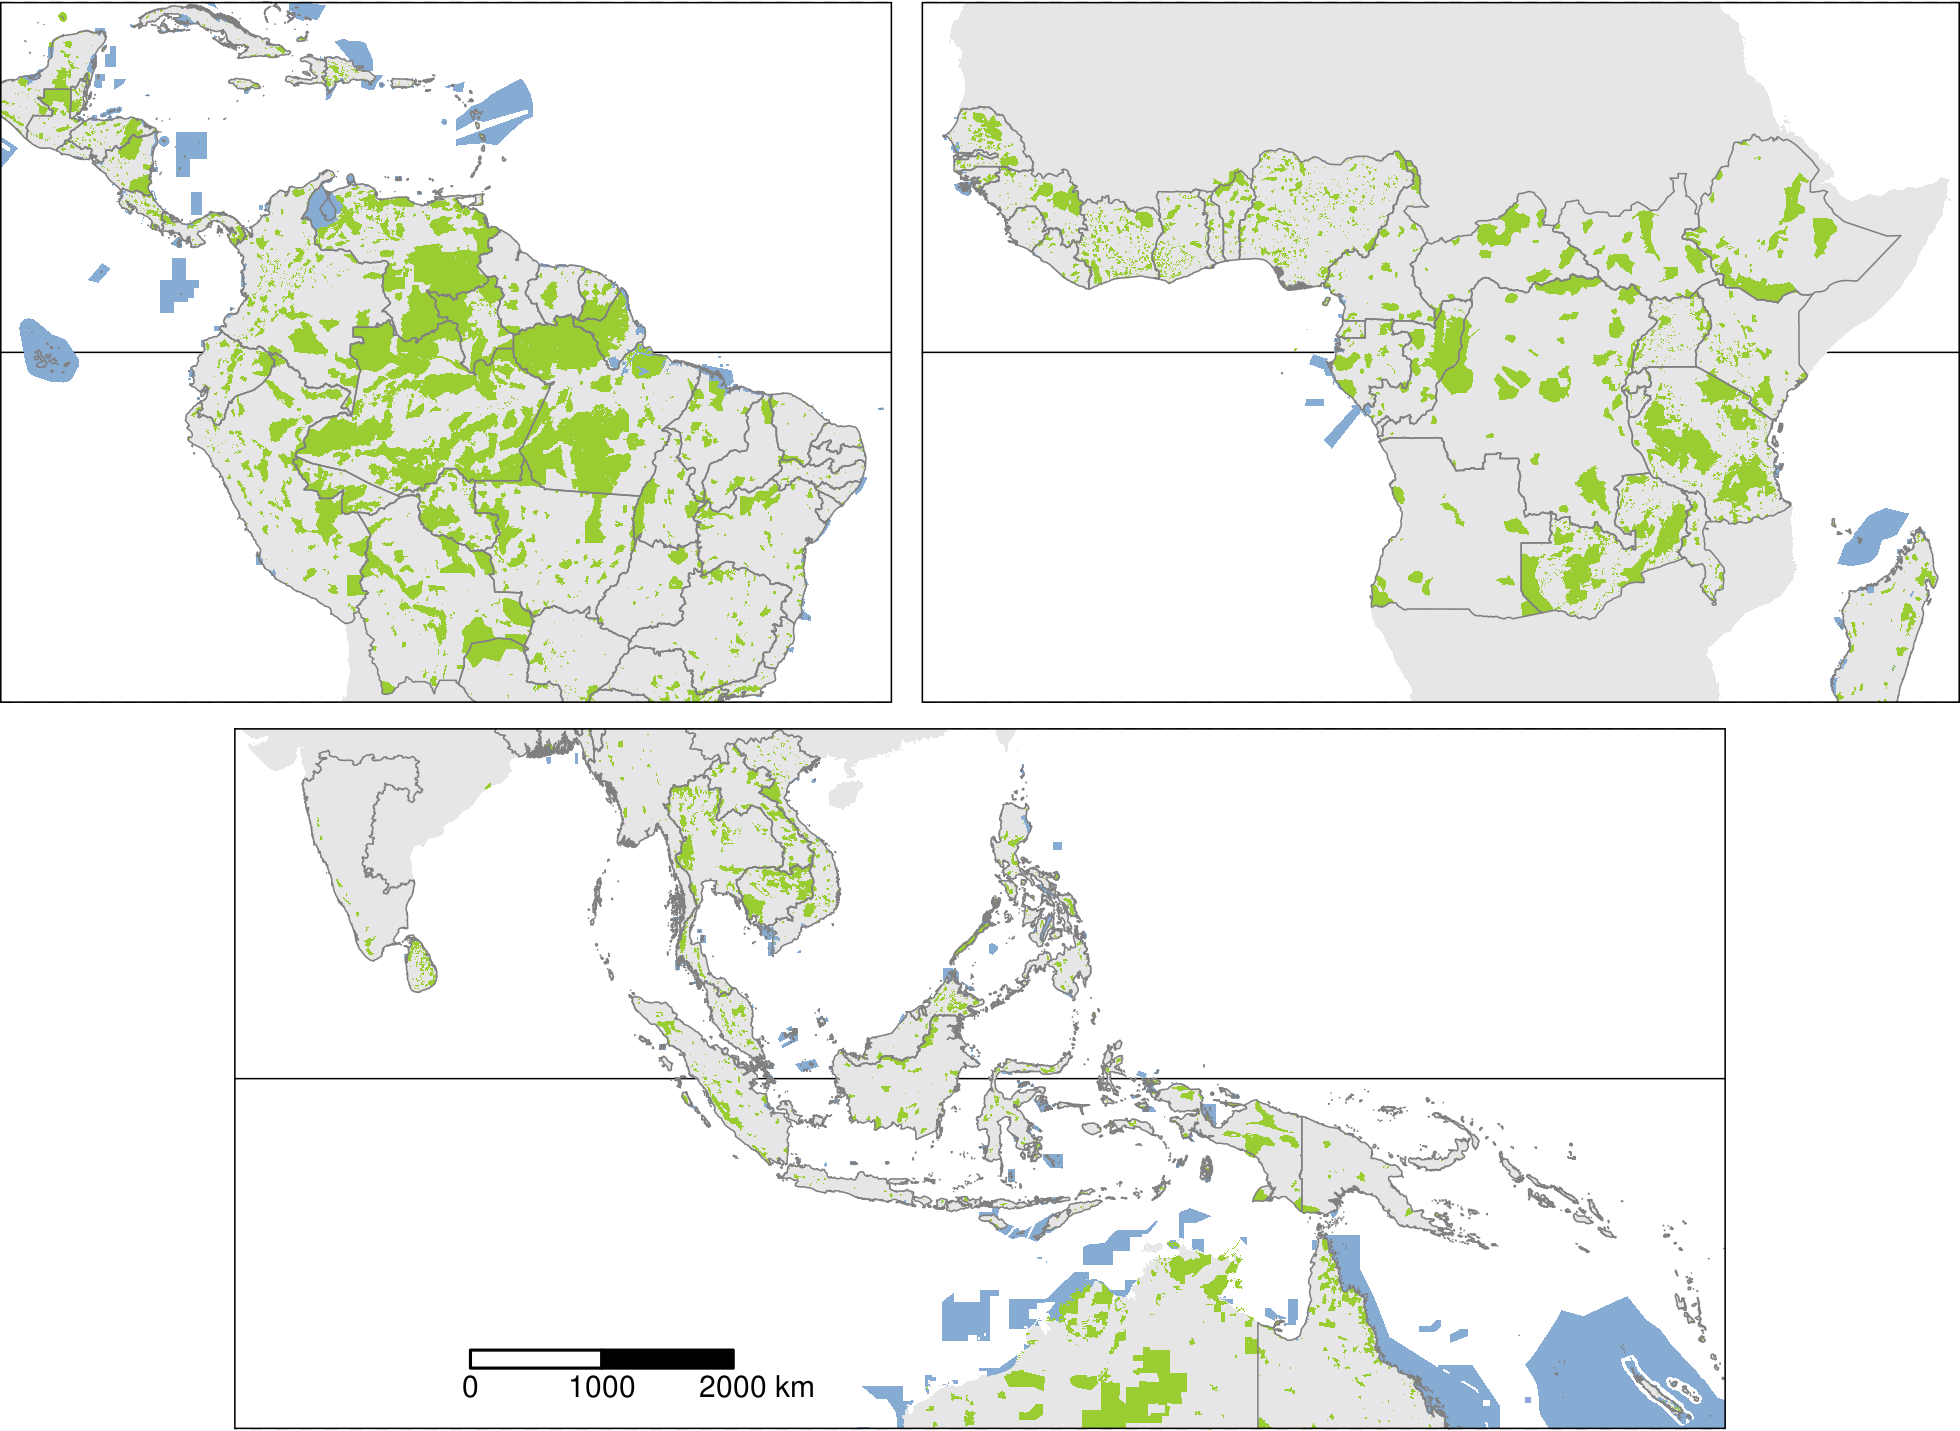
\includegraphics[width=0.7\textwidth]{figs/sm/pa.png}
\end{frame}

\begin{frame}[label={sec:org4b2e36c}]{Sampling}
One word on sampling:

\begin{itemize}
\item Stratified sampling between deforested/non-deforested pixels in
2010--2020
\item Total number of points proportional to the forest cover in 2010 (from
20,000 to 100,000 points per study area)
\item Huge data-set of 3.2 M forest pixels (\textasciitilde{}288 Kha of forest)
\end{itemize}

\centering 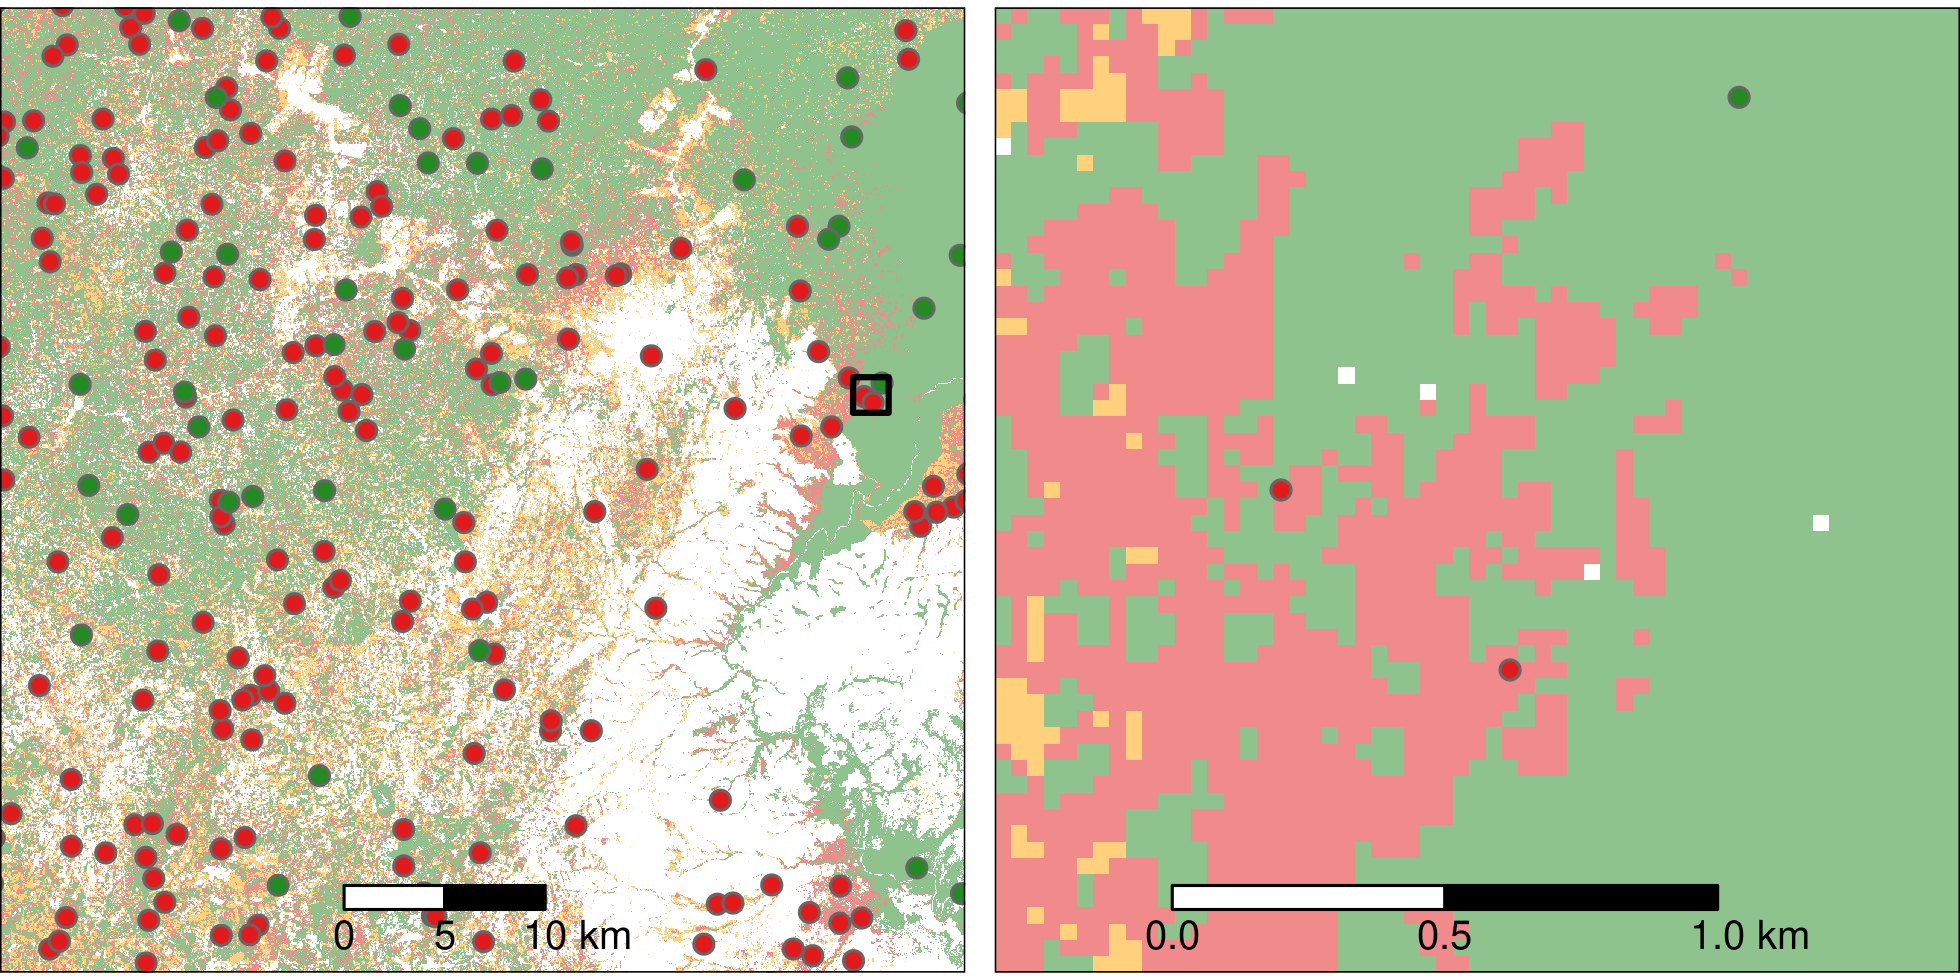
\includegraphics[width=0.7\textwidth]{figs/sm/sample.png}
\end{frame}

\subsection{Forecast}
\label{sec:org5c36b9f}
\begin{frame}[label={sec:orgd8c13c0}]{Spatial random effects}
\centering 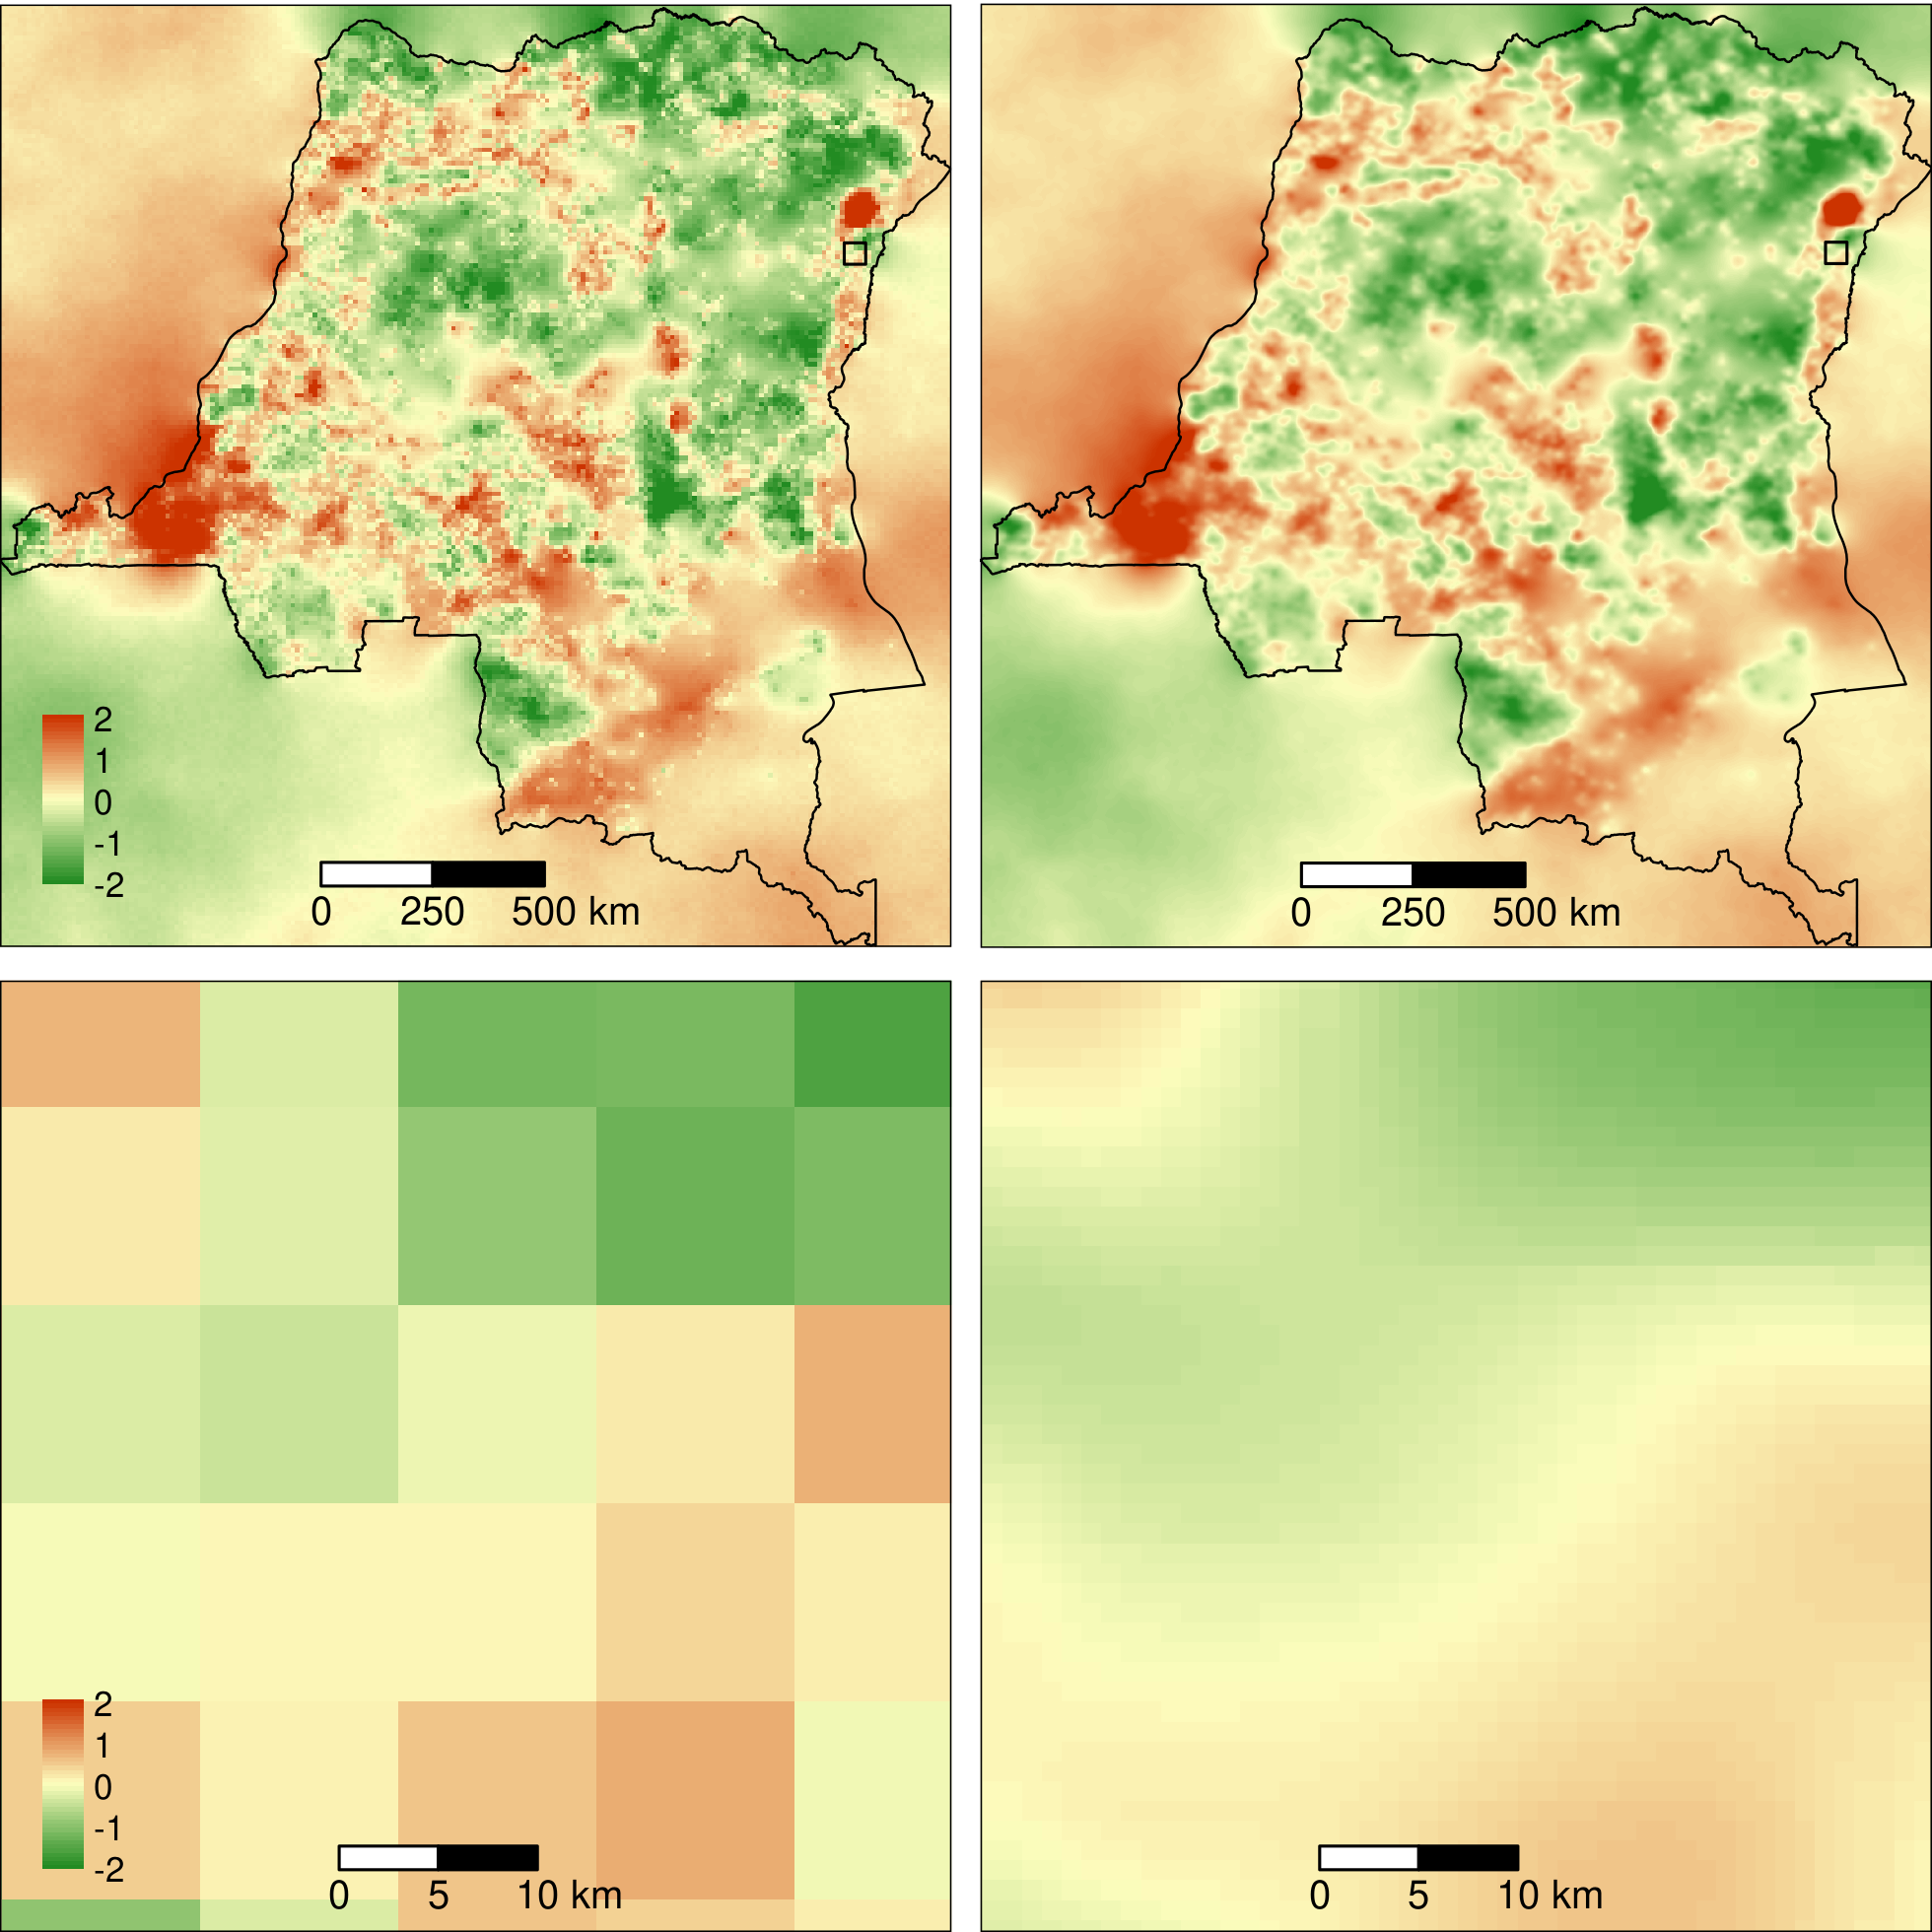
\includegraphics[width=0.6\textwidth]{figs/sm/rho.png}

\textbf{Interpolation of spatial random effects at 1km in DRC}
\end{frame}

\begin{frame}[label={sec:org0b59176}]{Spatial probability of deforestation}
We use the fitted model to compute the spatial probability of
deforestation.

\centering 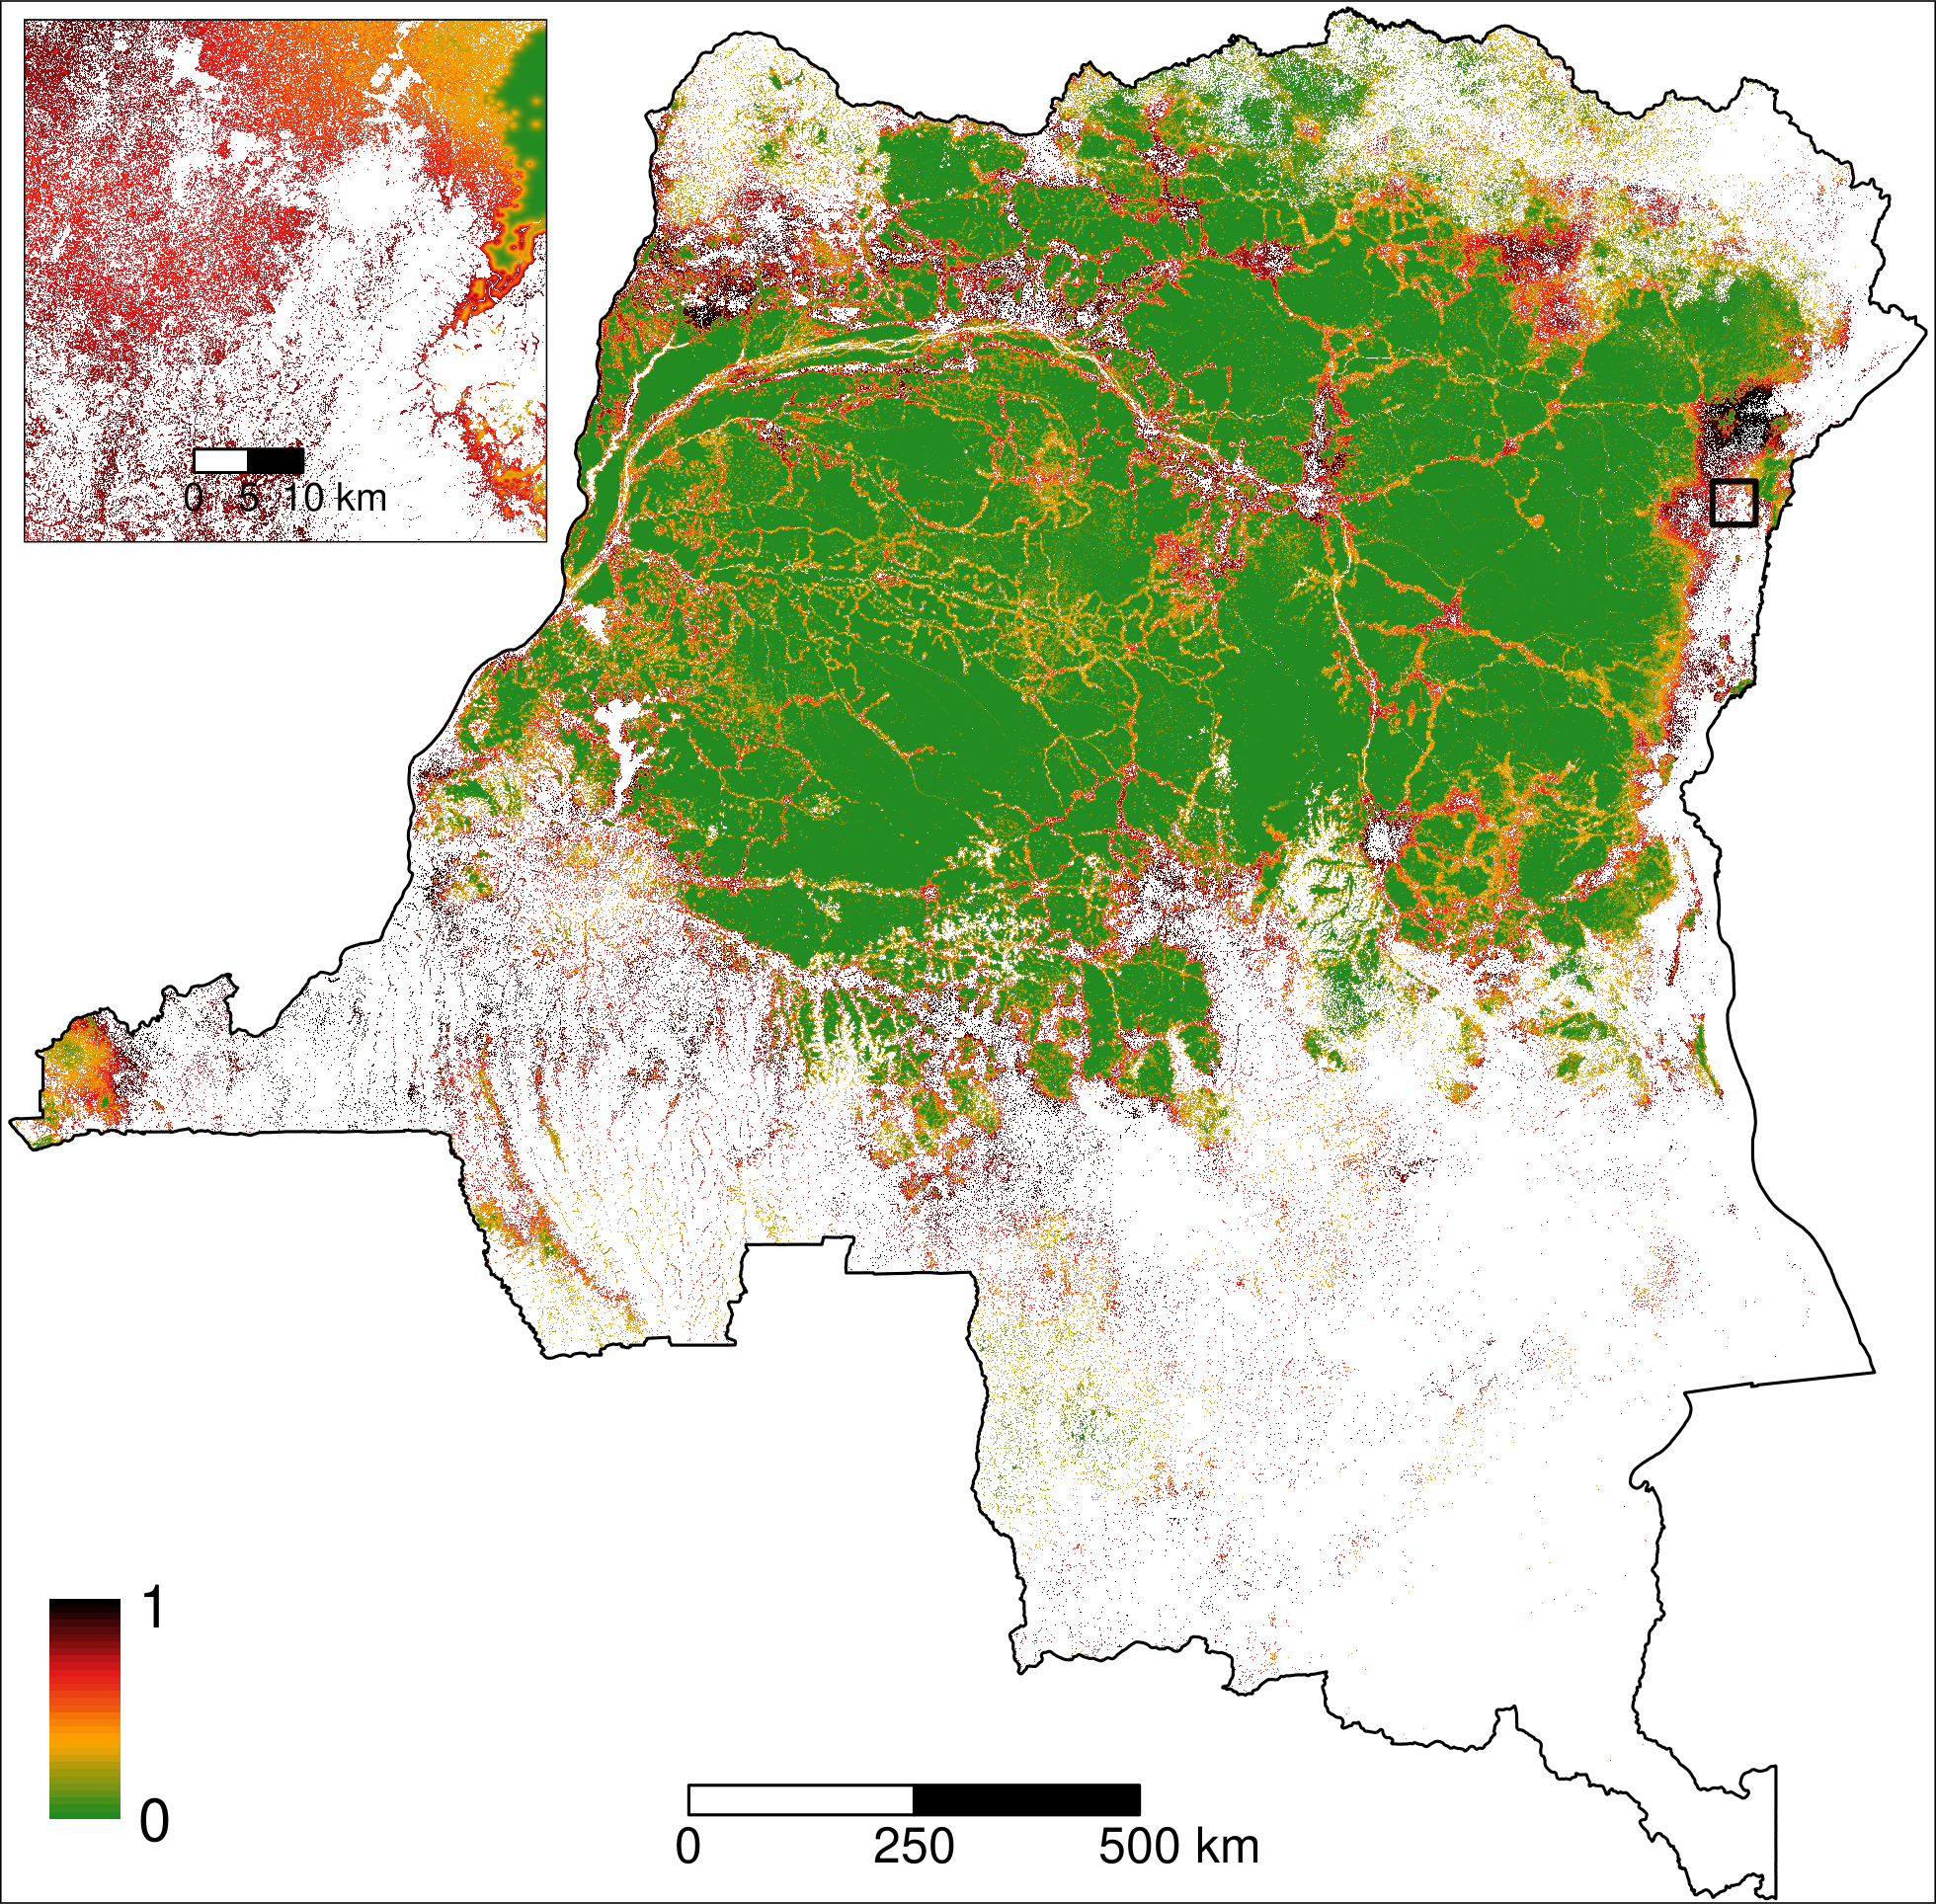
\includegraphics[width=0.5\textwidth]{figs/sm/prob.png}

\textbf{Relative spatial probability of deforestation in DRC for the year 2020}
\end{frame}

\begin{frame}[label={sec:orgc83c538}]{Spatial probability of deforestation}
\centering 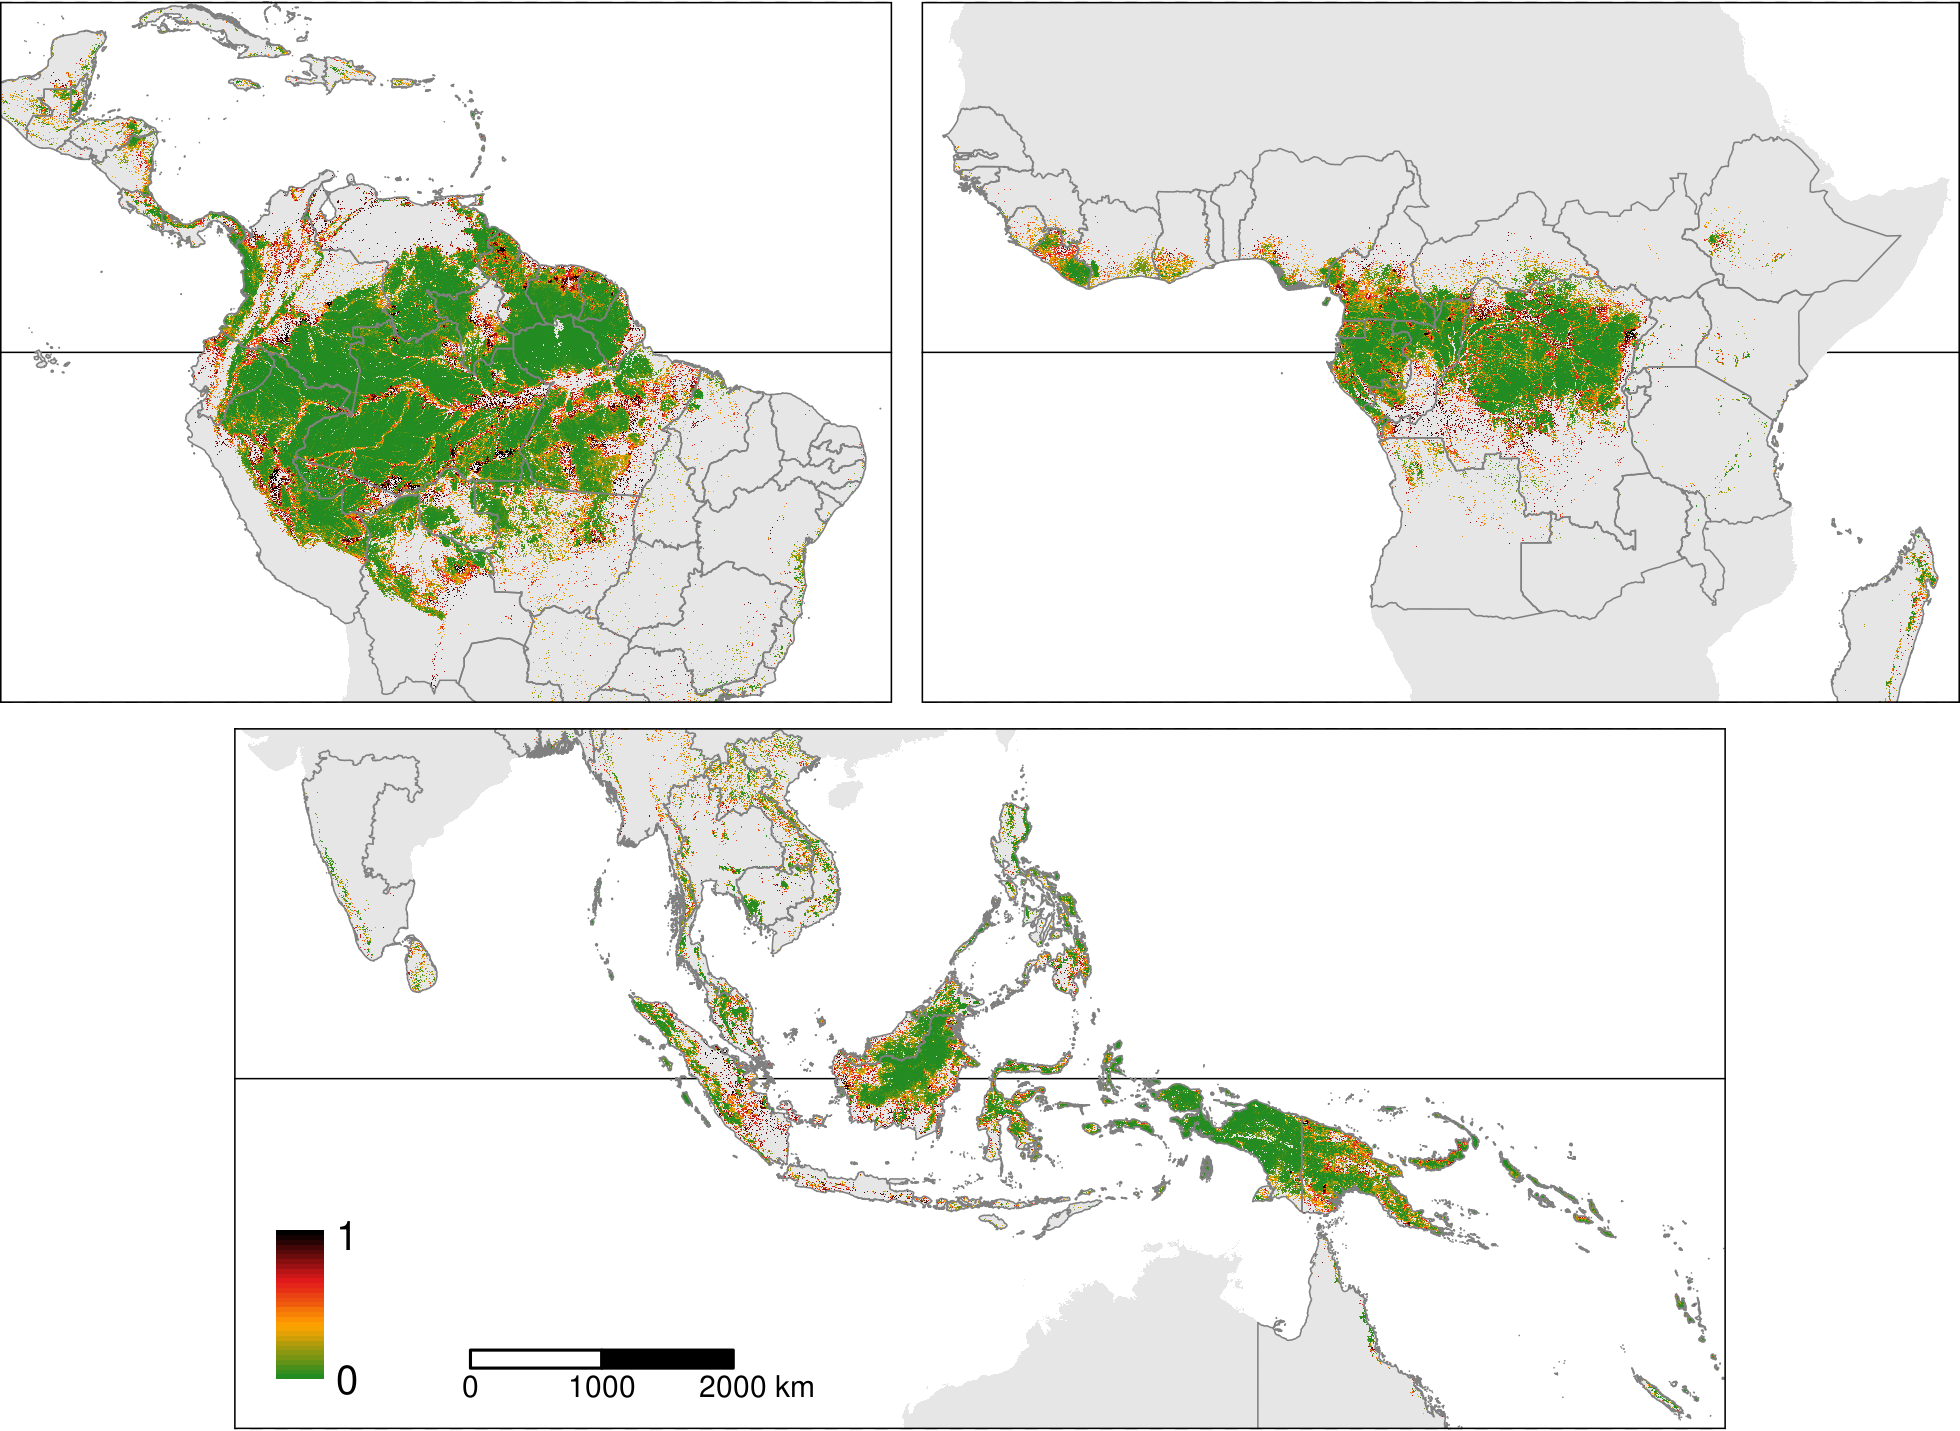
\includegraphics[width=0.8\textwidth]{figs/article/prob}

\textbf{Pantropical map of the spatial probability of deforestation}

\url{https://forestatrisk.cirad.fr/maps.html}
\end{frame}

\begin{frame}[label={sec:orgfb3d1d3}]{Future forest cover}
\begin{itemize}
\item Total deforested area \(D\) (ha) in a given period of time \(Y\) (yr):
\(D=d \times Y\), with \(d\) the annual deforested area (ha/yr).
\item Number of pixels to be deforested: \(n=D/0.09\), 0.09 ha being the
pixel area.
\item The \(n\) pixels with the highest deforestation probabilities are
considered deforested in that period of time.
\end{itemize}

\centering 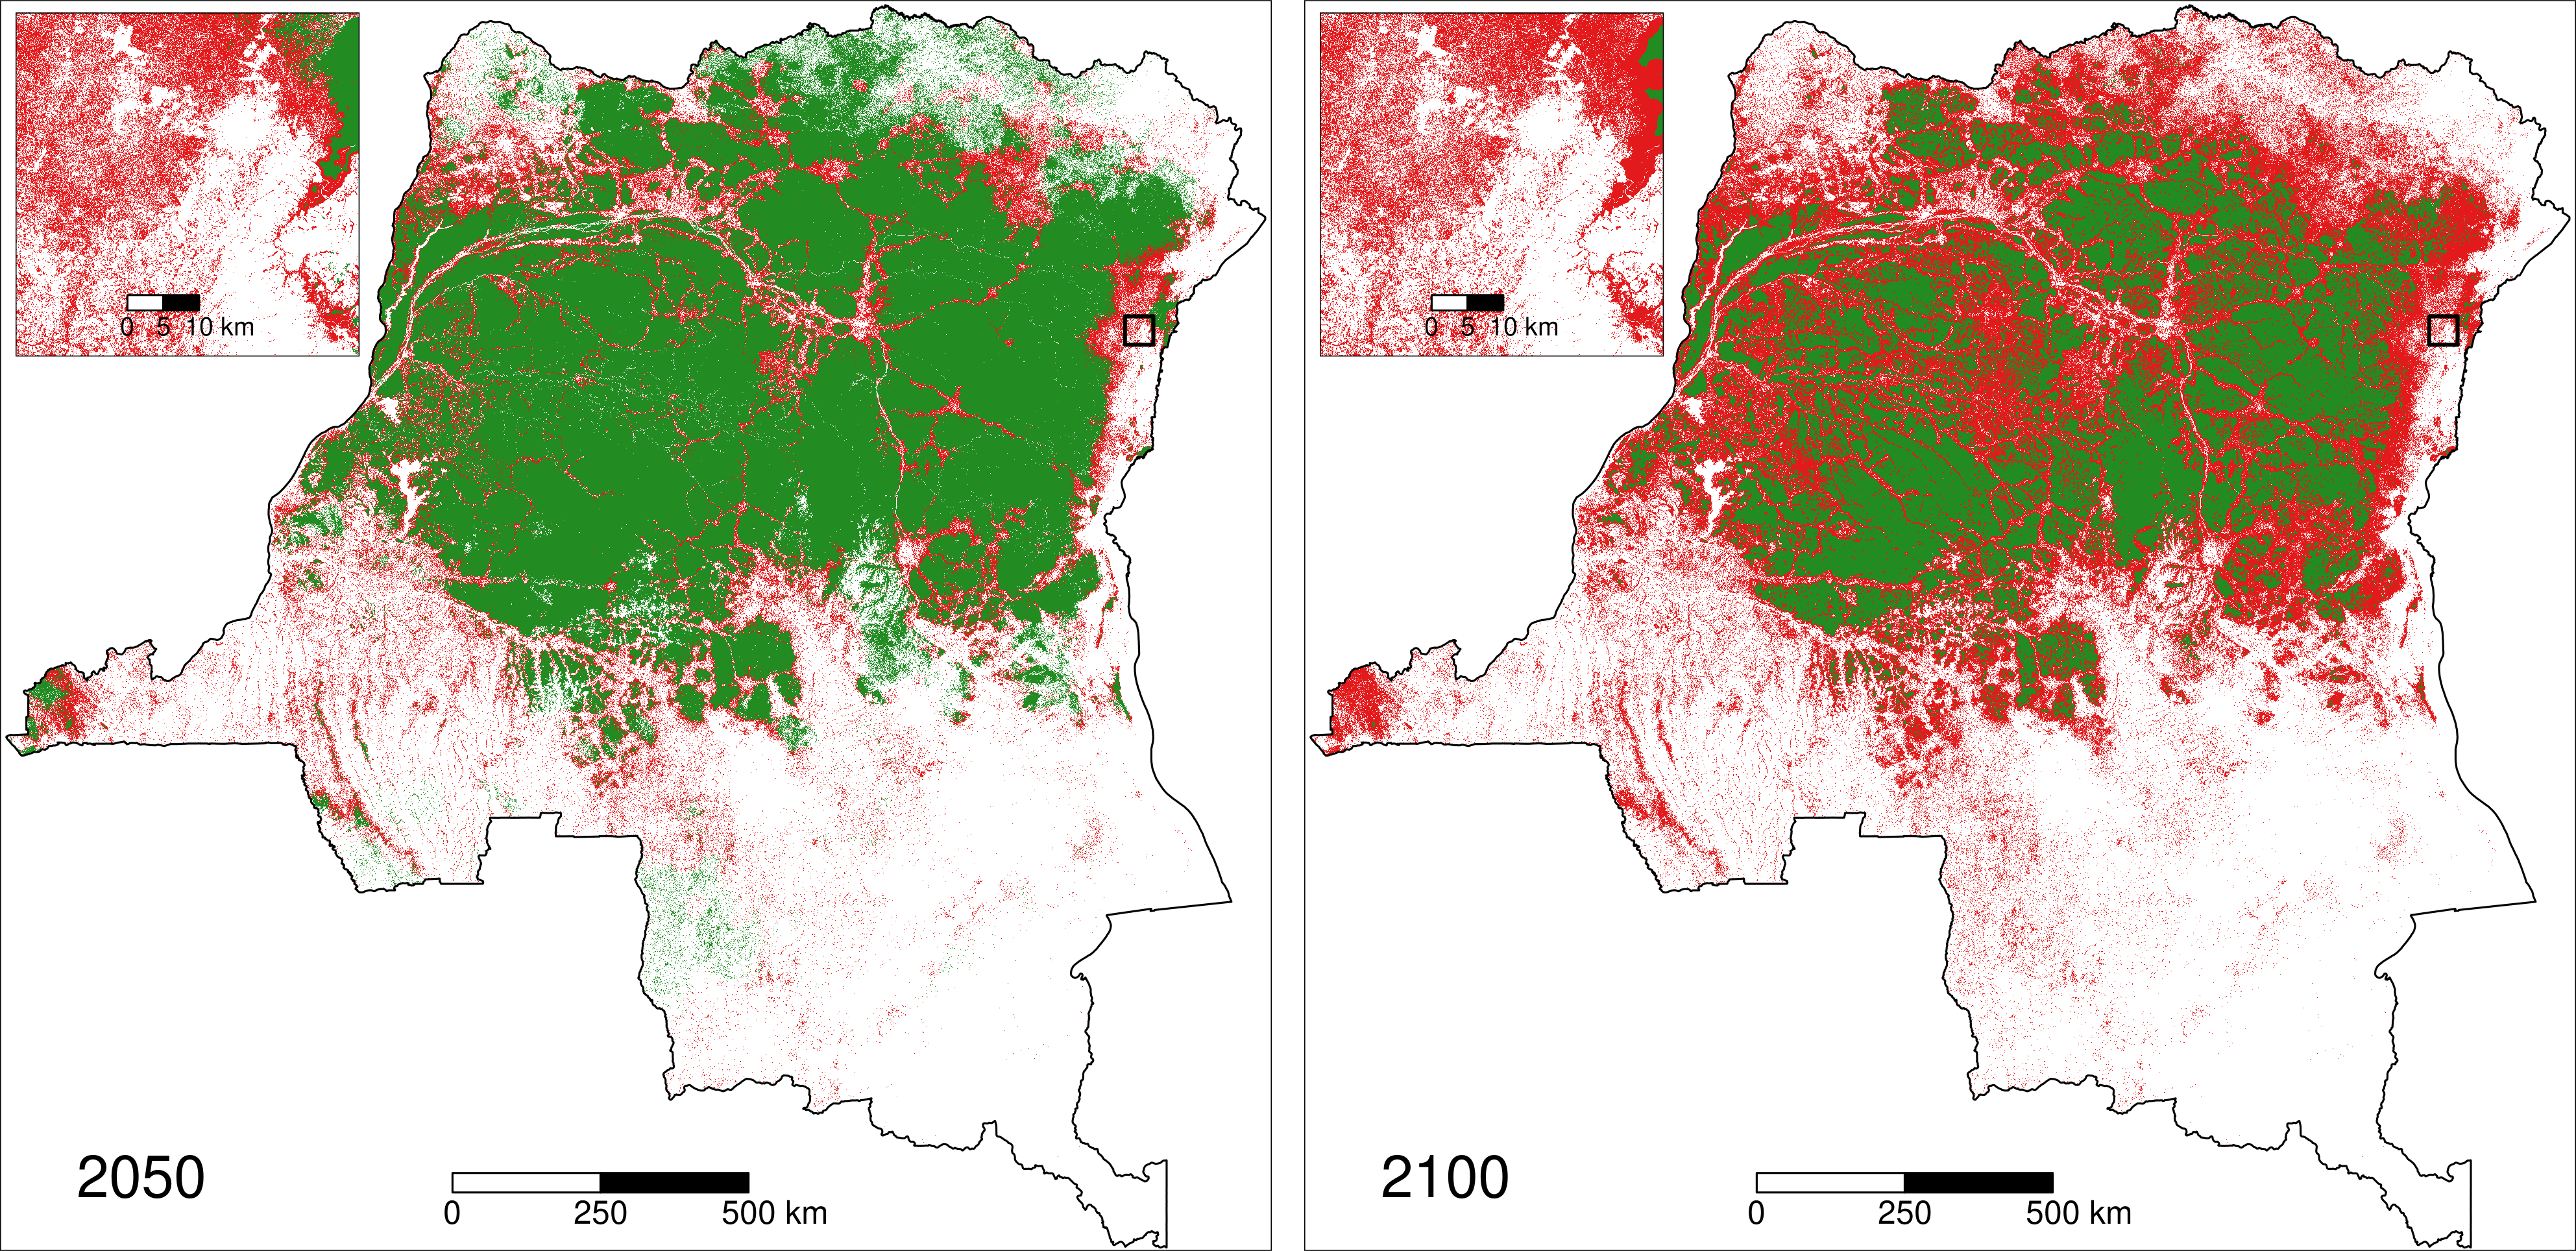
\includegraphics[width=0.7\textwidth]{figs/sm/fcc2050_2100.png}

\textbf{Projected deforestation in 2020--2050 and 2020--2100 in DRC}
\end{frame}

\begin{frame}[label={sec:orgc1153bb}]{Future carbon emissions}
\begin{columns}
\begin{column}{0.5\columnwidth}
\begin{itemize}
\item Projected deforestation for years 2030, 2040, \ldots{}, 2100.
\item We combine the maps of the projected deforestation with the
(2000--2010) forest carbon map by Avitabile 2016 GCB (1km resolution).
\end{itemize}
\end{column}

\begin{column}{0.5\columnwidth}
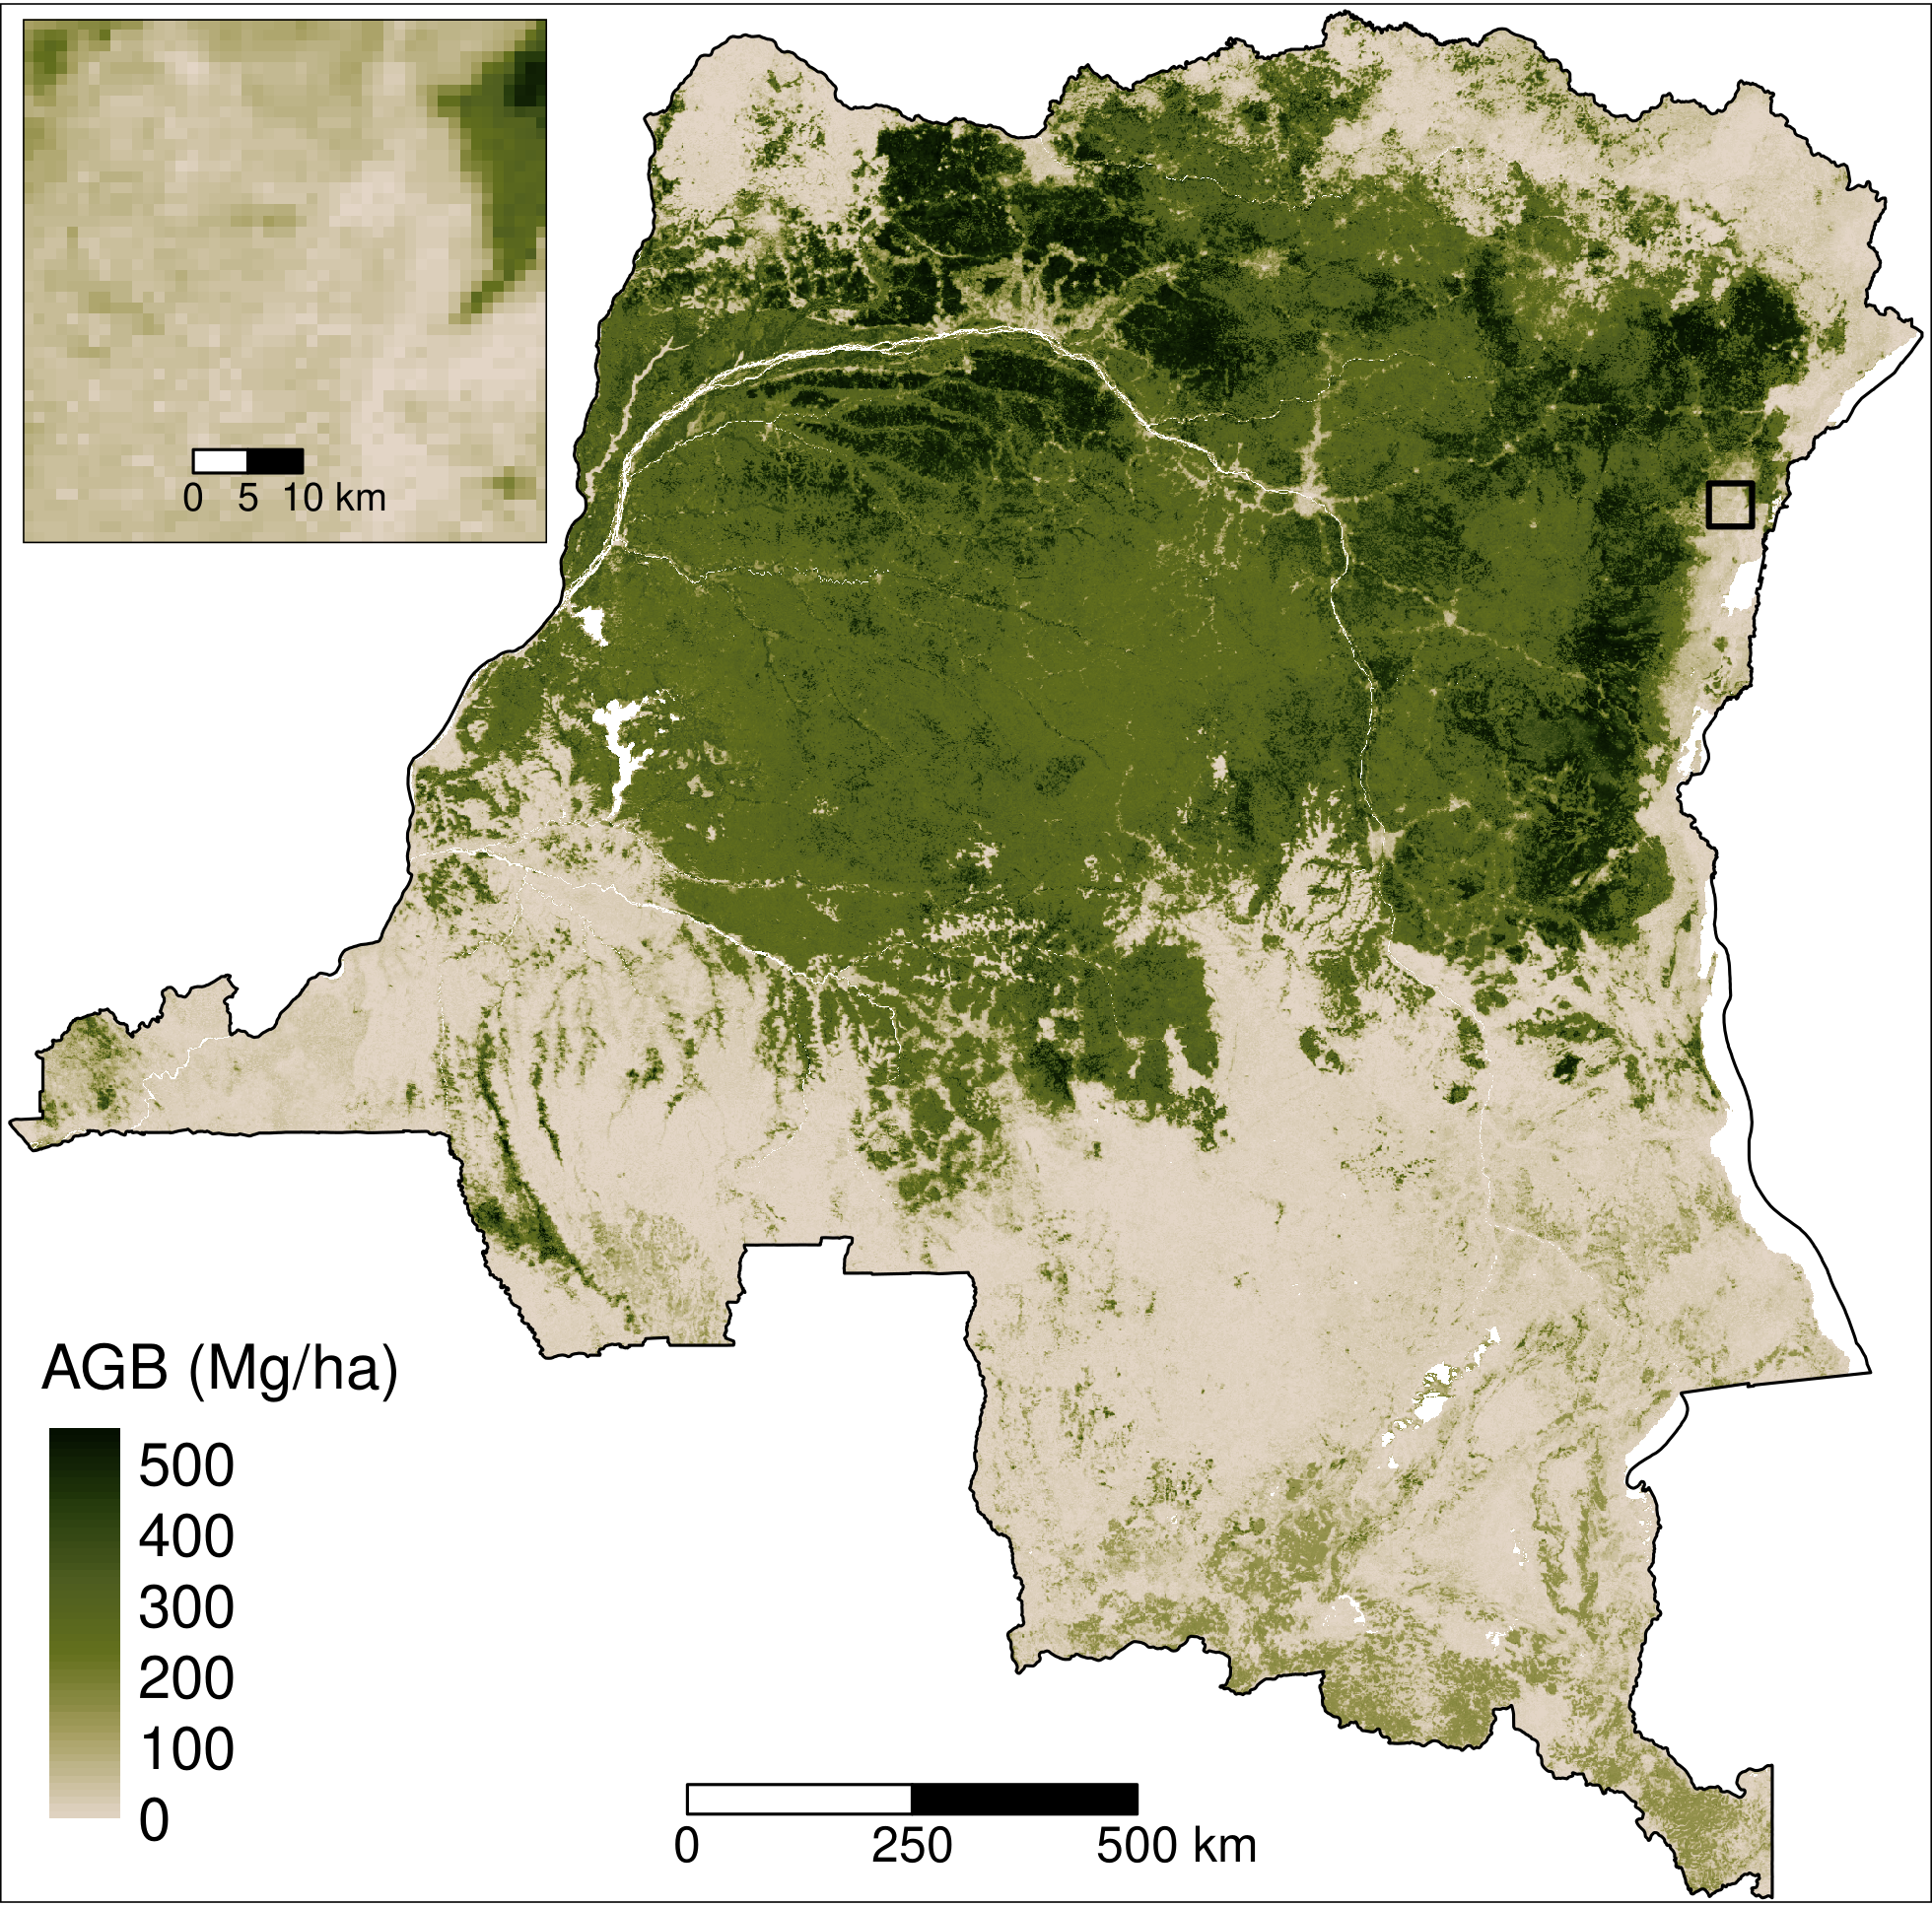
\includegraphics[width=\textwidth]{figs/sm/AGB}

\textbf{Aboveground biomass in DRC}
\end{column}
\end{columns}
\end{frame}

\begin{frame}[label={sec:org8ca7df7},fragile]{Software}
 \begin{itemize}
\item \texttt{forestatrisk} Python package
\item Process large rasters by blocks
\item Several statistical models: iCAR, GLM, RF, etc.
\item Set of functions for sampling, modelling, forecasting, validating
\end{itemize}

\begin{center}
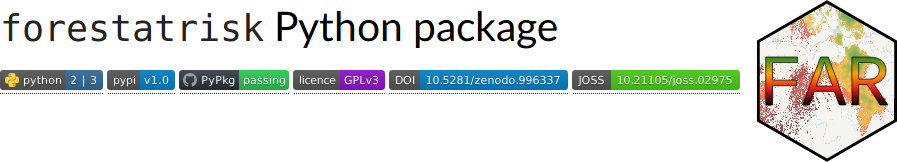
\includegraphics[width=0.8\textwidth]{figs/far-Python}\\
Website: \url{https://ecology.ghislainv.fr/forestatrisk}\\
Article: \textbf{Vieilledent} 2021, \emph{JOSS}, doi: \href{https://doi.org/10.21105/joss.02975}{10.21105/joss.02975}
\end{center}
\end{frame}

\section{Results}
\label{sec:org0026d3d}
\subsection{Forest refuge areas}
\label{sec:org2c4b0eb}
\begin{frame}[label={sec:orgc27eb72}]{Tropical forest cover loss}
\small
75\% of the tropical forest existing in 2000 will be lost in 2120, 2160,
and 2220 in Asia, Africa, and America, respectively (average uncertainty of \textpm{}45 years).

\centering 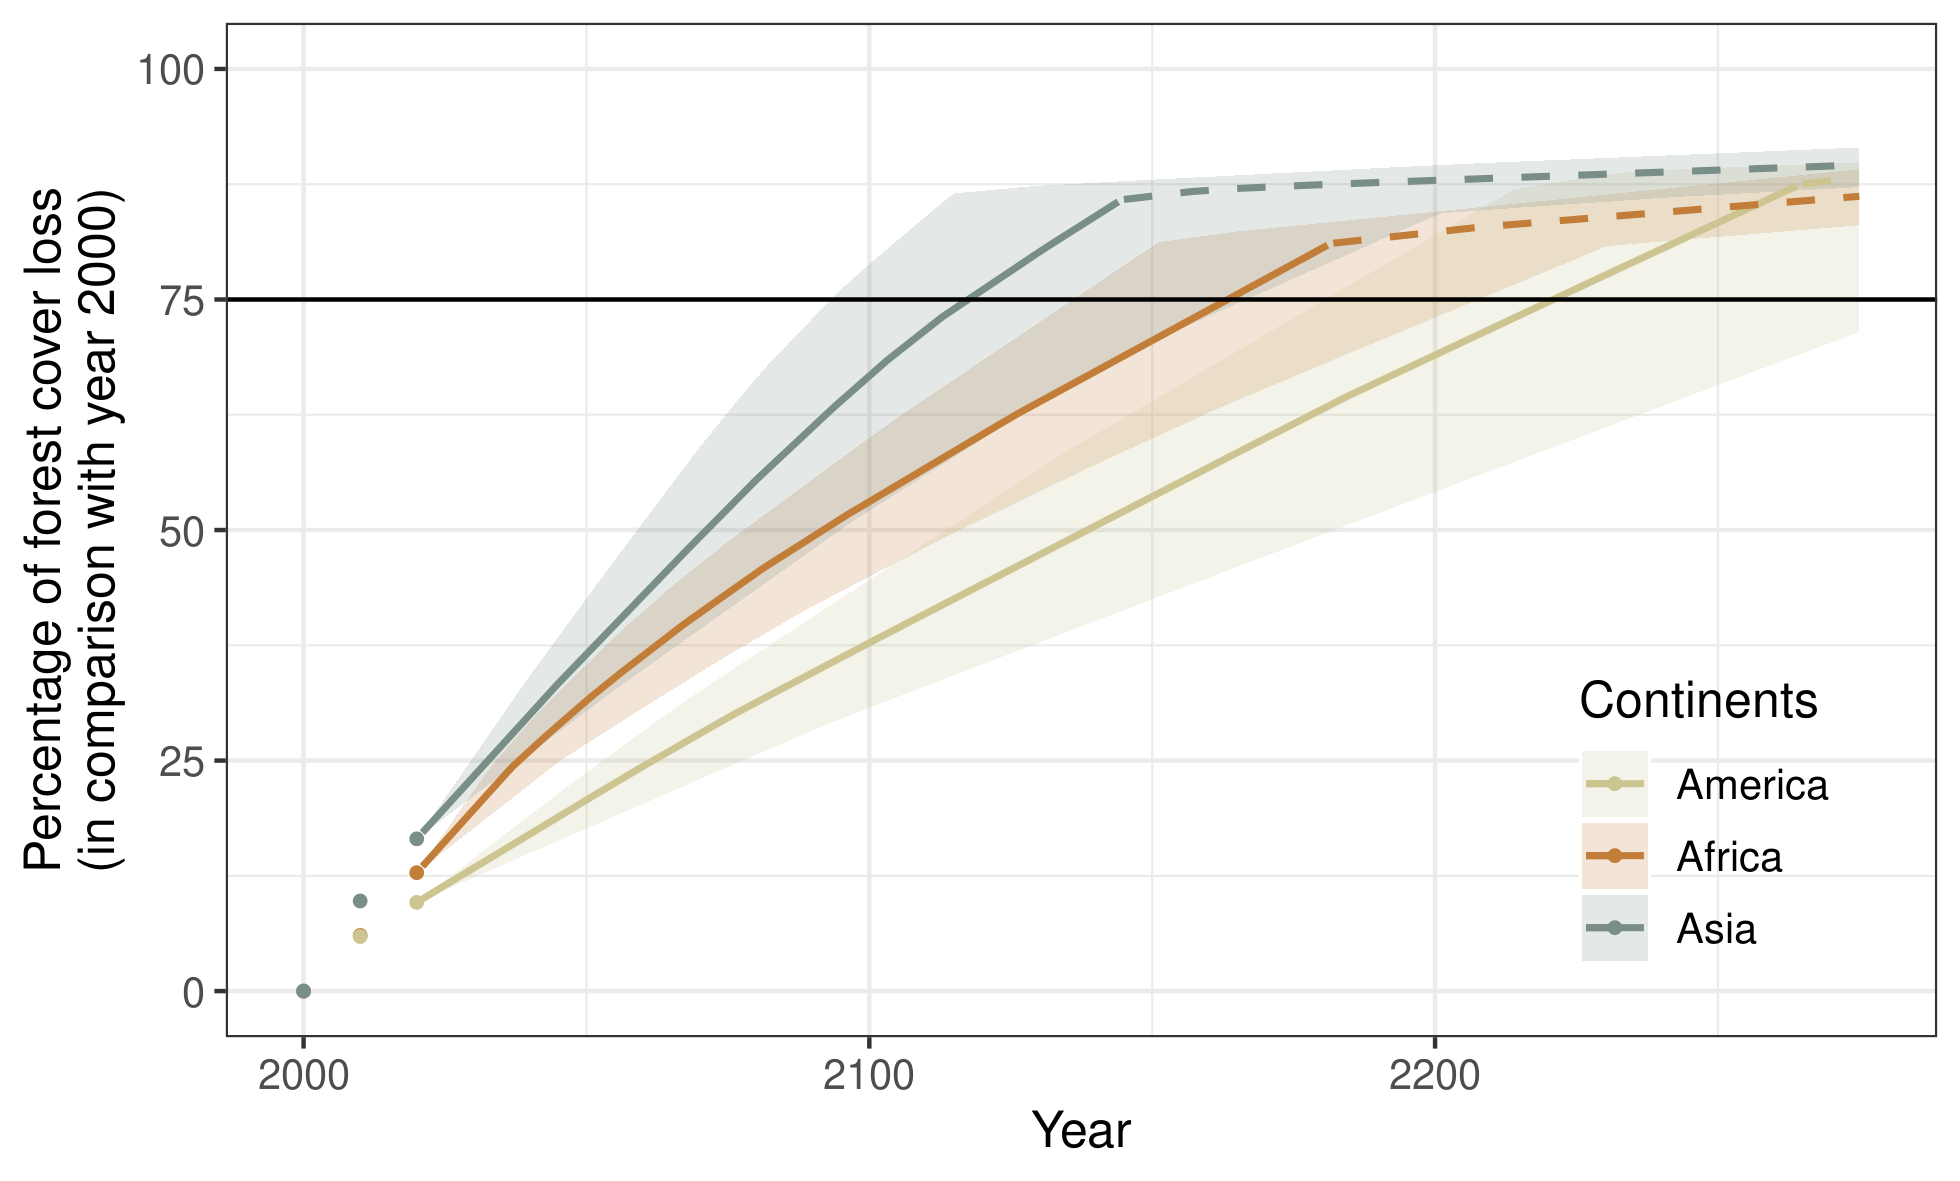
\includegraphics[width=0.8\textwidth]{figs/article/perc_loss_cont}
\end{frame}

\begin{frame}[label={sec:org9a585f5}]{Tropical forest cover loss}
\small
\begin{itemize}
\item 20 countries, 5 states in Brazil, and 1 region in India (having > 1
Mha of forest in 2020) will lose all their tropical forest by 2100.
\item No more tropical forests in 6 biodiversity hotspots (extinction of
29,140 endemic species of plants and 4,576 species of vertebrates).
\end{itemize}

\centering 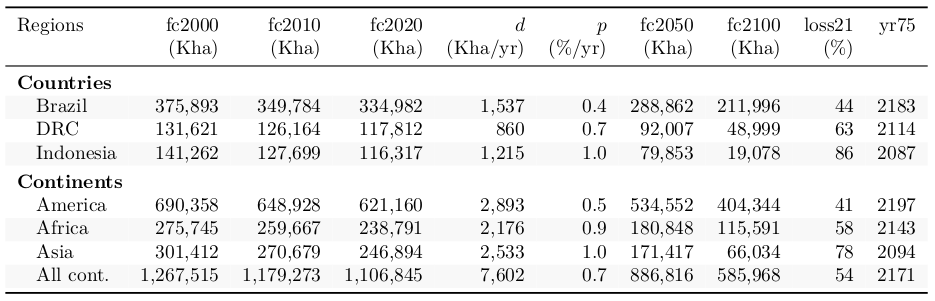
\includegraphics[width=0.8\textwidth]{figs/defor-tab}
\end{frame}

\begin{frame}[label={sec:orgcbed510}]{Pantropical map of the future forest cover}
\small
Tropical forests in 2100 will be (i) highly fragmented, (ii)
concentrated in remote areas (far from roads and towns), pref. in
protected areas, and at high elevations.

\centering 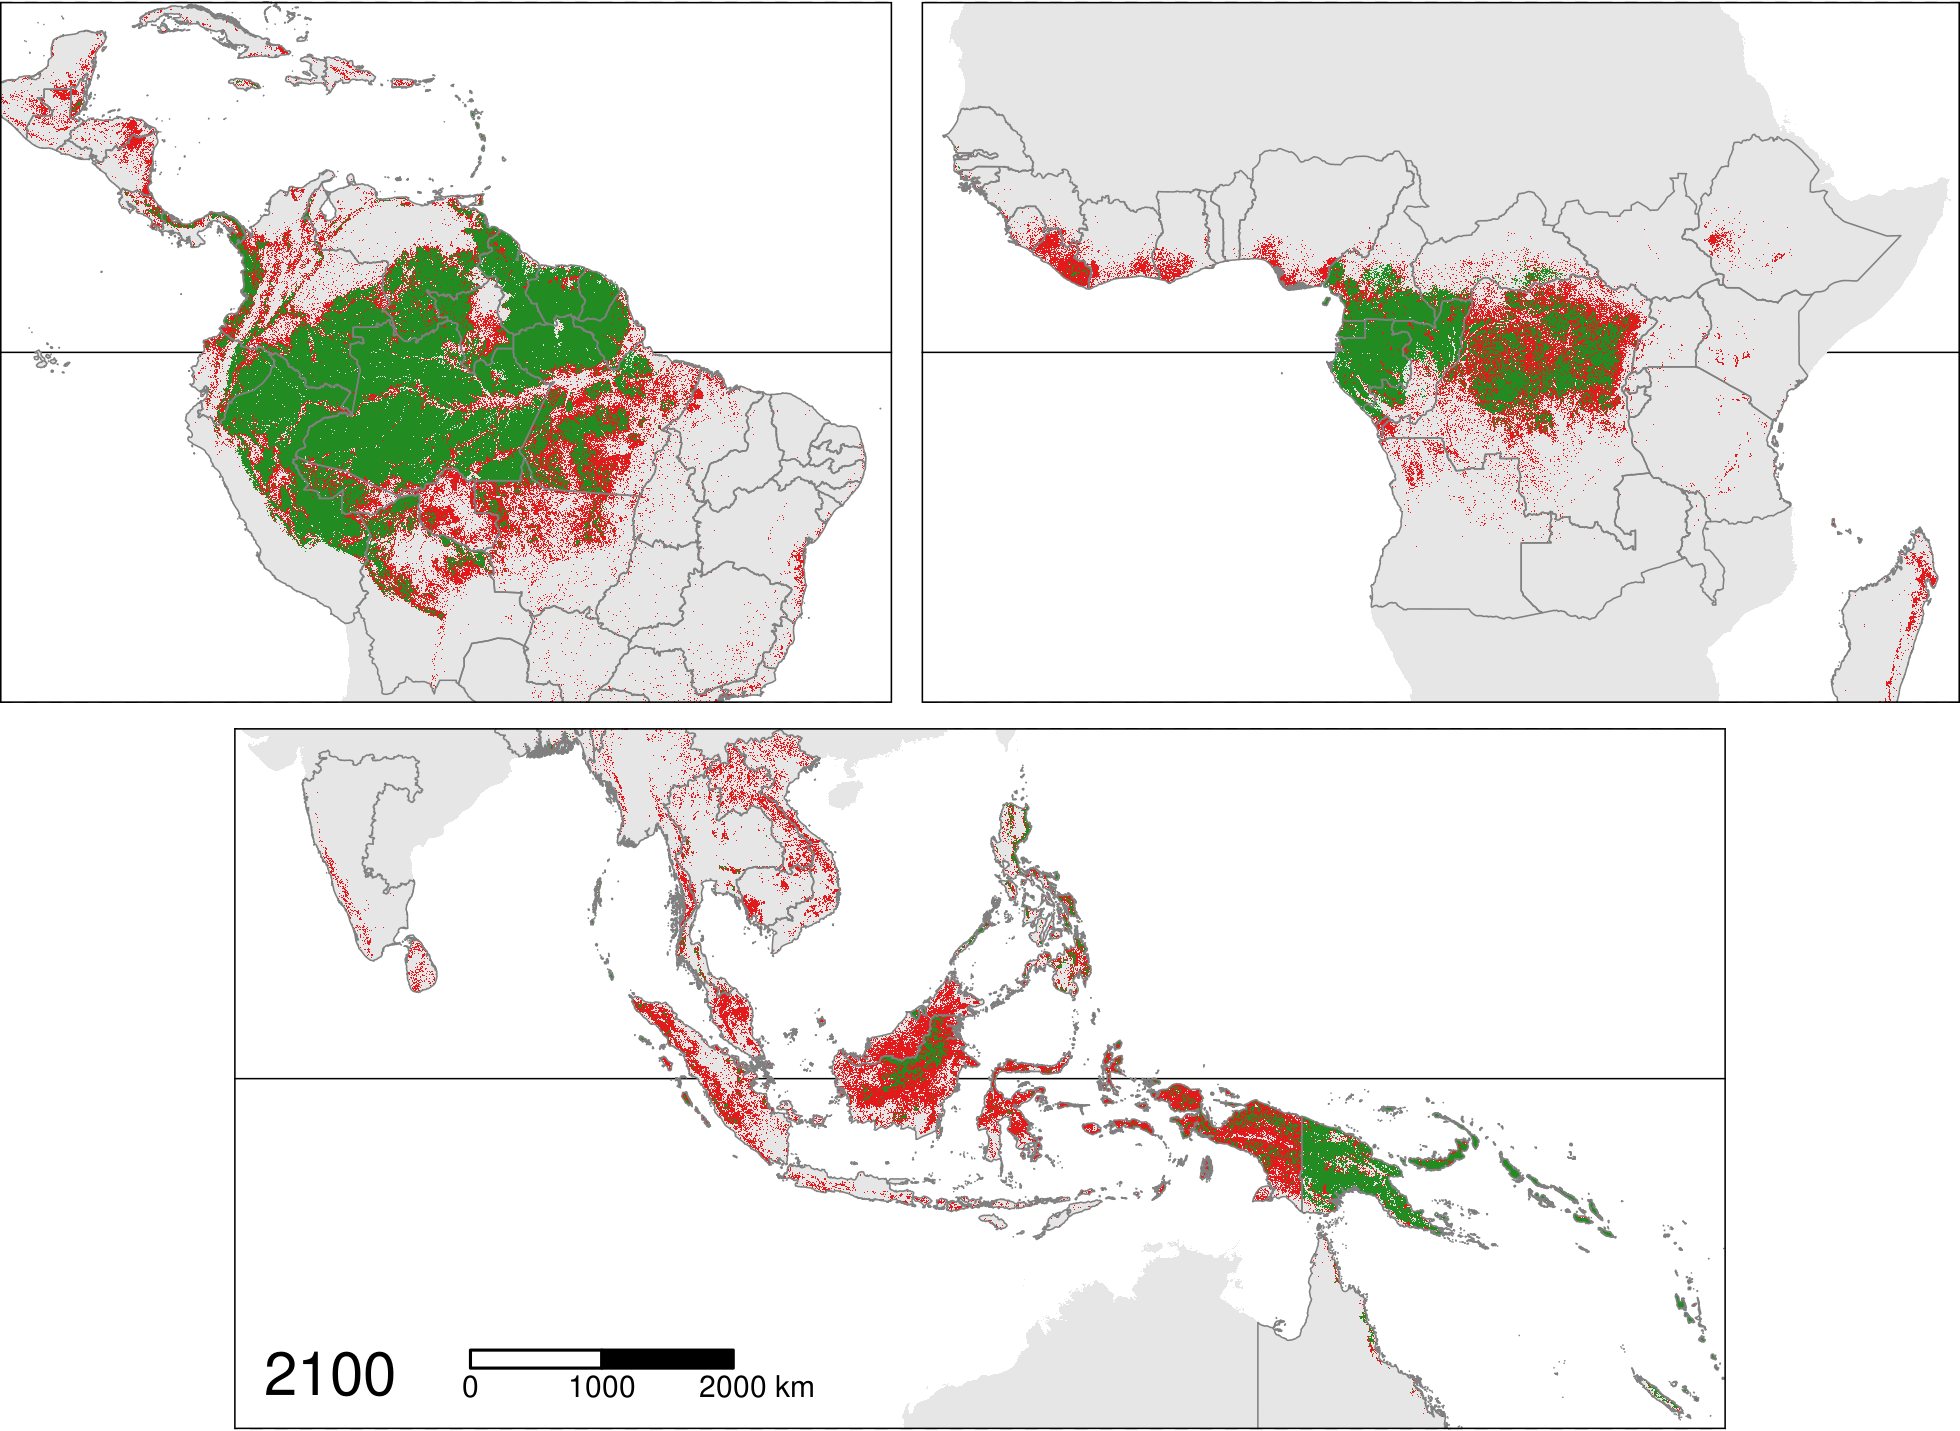
\includegraphics[width=0.7\textwidth]{figs/article/fcc2100}

\textbf{Pantropical map of future forest cover in 2100}

\url{https://forestatrisk.cirad.fr/maps.html}
\end{frame}

\subsection{Carbon emissions}
\label{sec:org9d43354}
\begin{frame}[label={sec:org678b051}]{Carbon emissions}
\begin{itemize}
\item Future deforestation will impact forests with higher carbon stocks
\item Annual carbon emissions will increase from 0.525 Pg/yr in 2010--2020
to 0.746 Pg/yr in 2070--2080 (42\% increase)
\end{itemize}

\centering 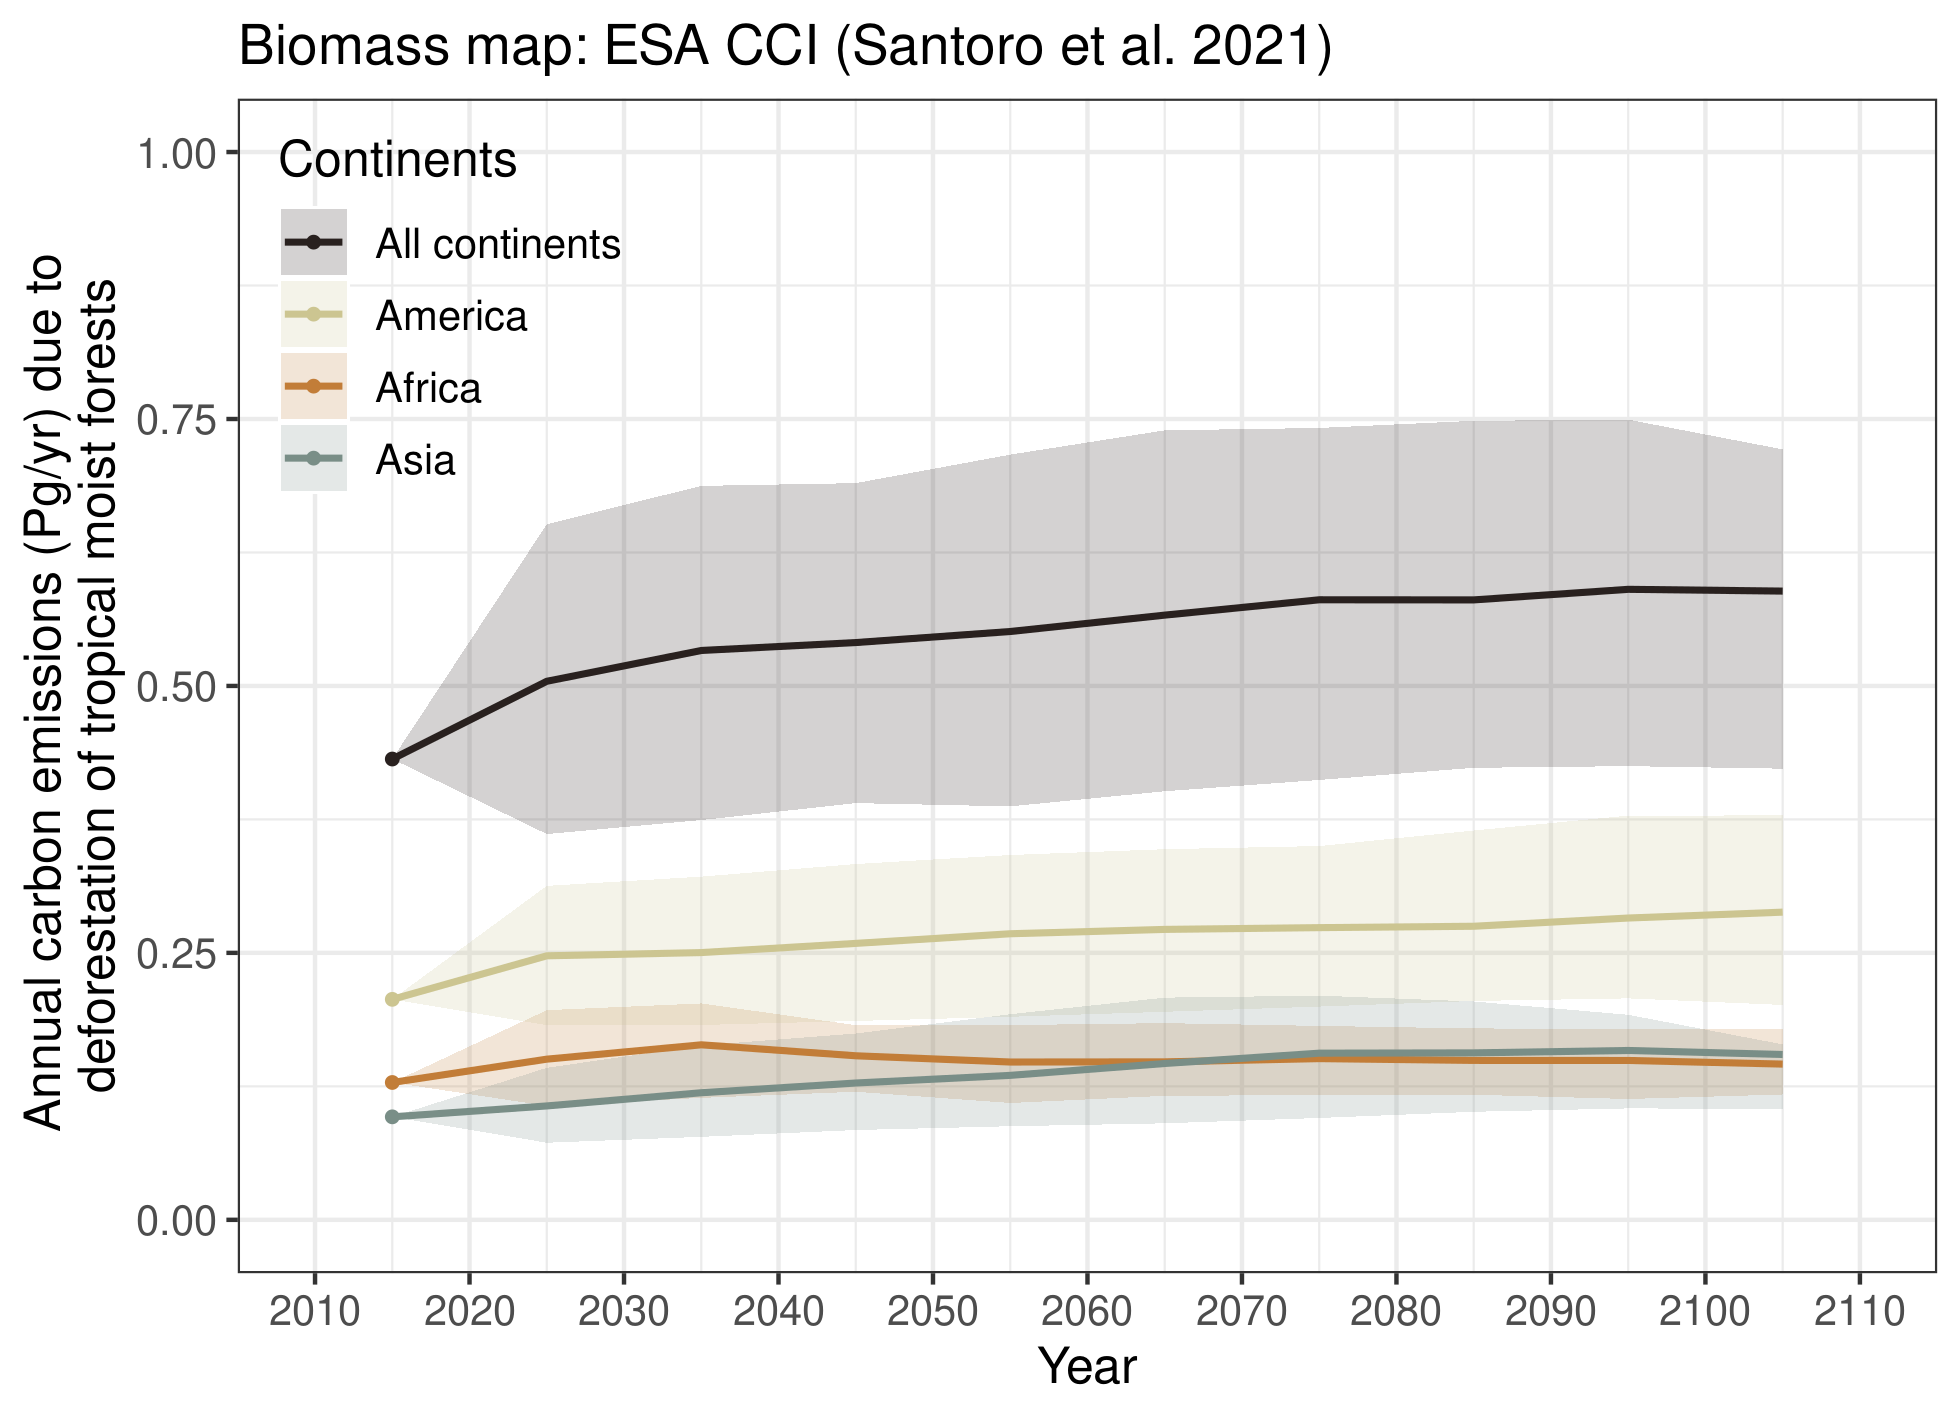
\includegraphics[width=0.8\textwidth]{figs/article/C_trend}

\textbf{Carbon emissions from future deforestation}
\end{frame}

\subsection{Effects of PA and roads}
\label{sec:org33fbdc8}
\begin{frame}[label={sec:orgb3d2659}]{Protected area effect}
\begin{columns}
\begin{column}{0.5\columnwidth}
\begin{itemize}
\item Significant PA effect in 74 study areas out of 119 (88\% of the TMF in
2010).
\item PA reduce the risk of deforestation by 40\%.
\end{itemize}
\end{column}

\begin{column}{0.5\columnwidth}
\centering 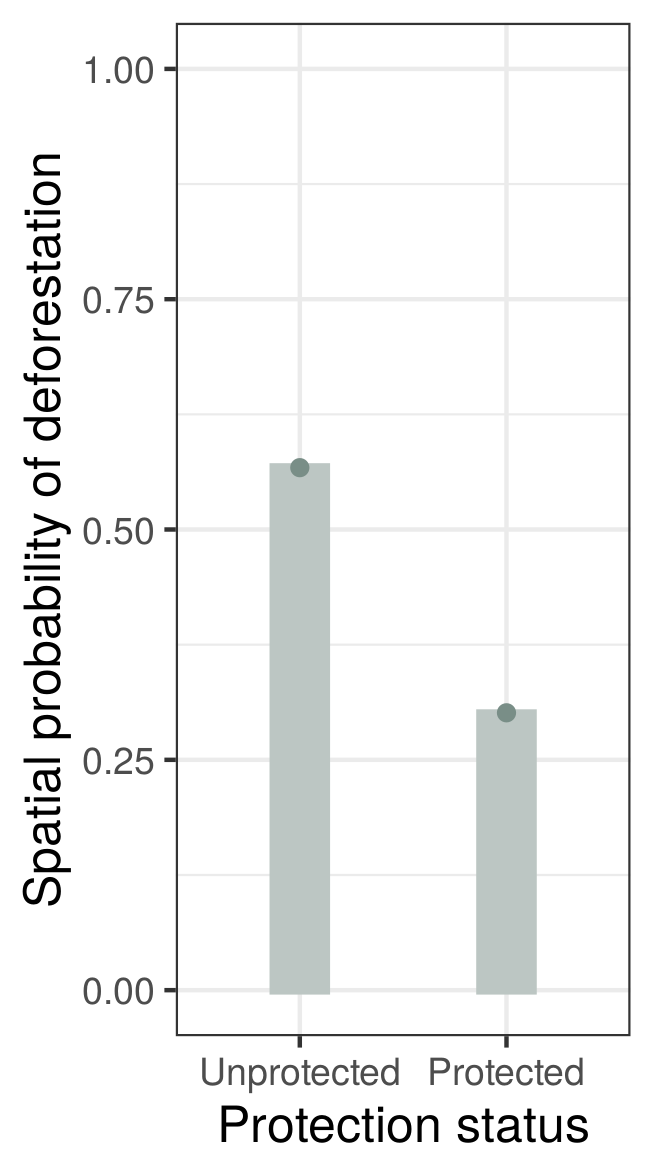
\includegraphics[width=0.65\textwidth]{figs/article/proba-PA}

\textbf{Effect of PA on the deforestation risk}
\end{column}
\end{columns}
\end{frame}

\begin{frame}[label={sec:orgcb55f1c}]{Road effect}
\begin{columns}
\begin{column}{0.5\columnwidth}
\begin{itemize}
\item Significant road effect in 59 study areas out of 119 (90\% of the TMF
in 2010).
\item At 10km from a road, the risk of deforestation decreases by 13\%.
\end{itemize}
\end{column}

\begin{column}{0.5\columnwidth}
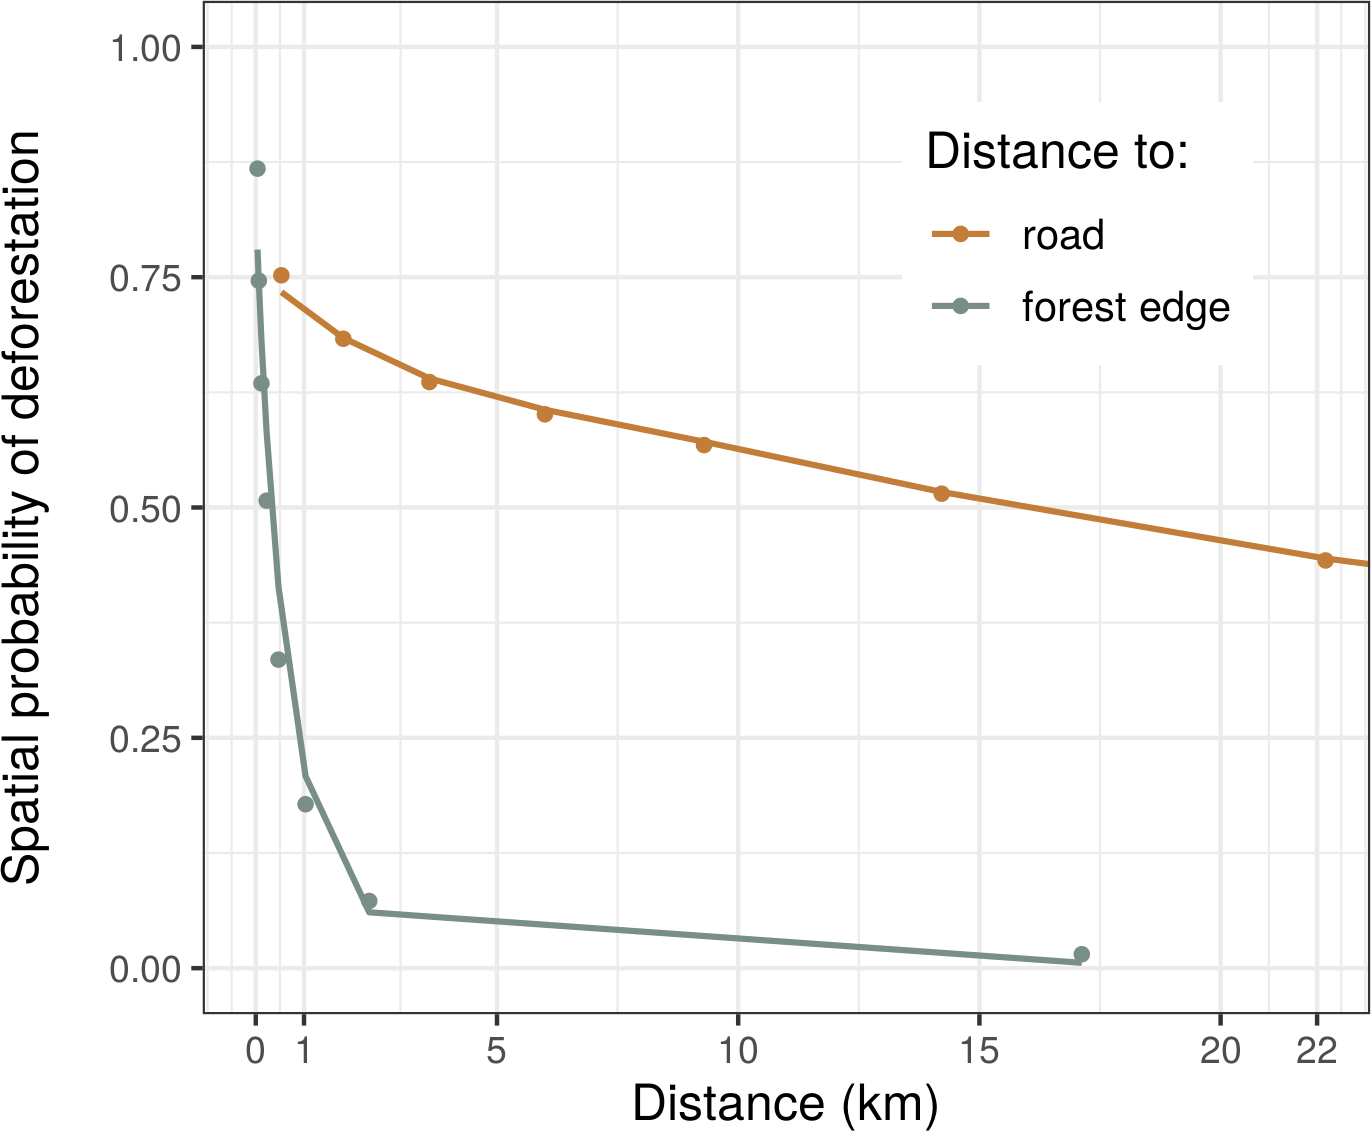
\includegraphics[width=\textwidth]{figs/article/proba-roads}

\textbf{Effects of roads and forest edge on the deforestation risk}
\end{column}
\end{columns}
\end{frame}

\begin{frame}[label={sec:org15252b5}]{Forest edge effect}
\begin{columns}
\begin{column}{0.5\columnwidth}
\begin{itemize}
\item Road effect must be interpreted together with forest edge effect.
\item At 1km from the forest edge, the risk of deforestation decreases by
93\%.
\end{itemize}
\end{column}

\begin{column}{0.5\columnwidth}
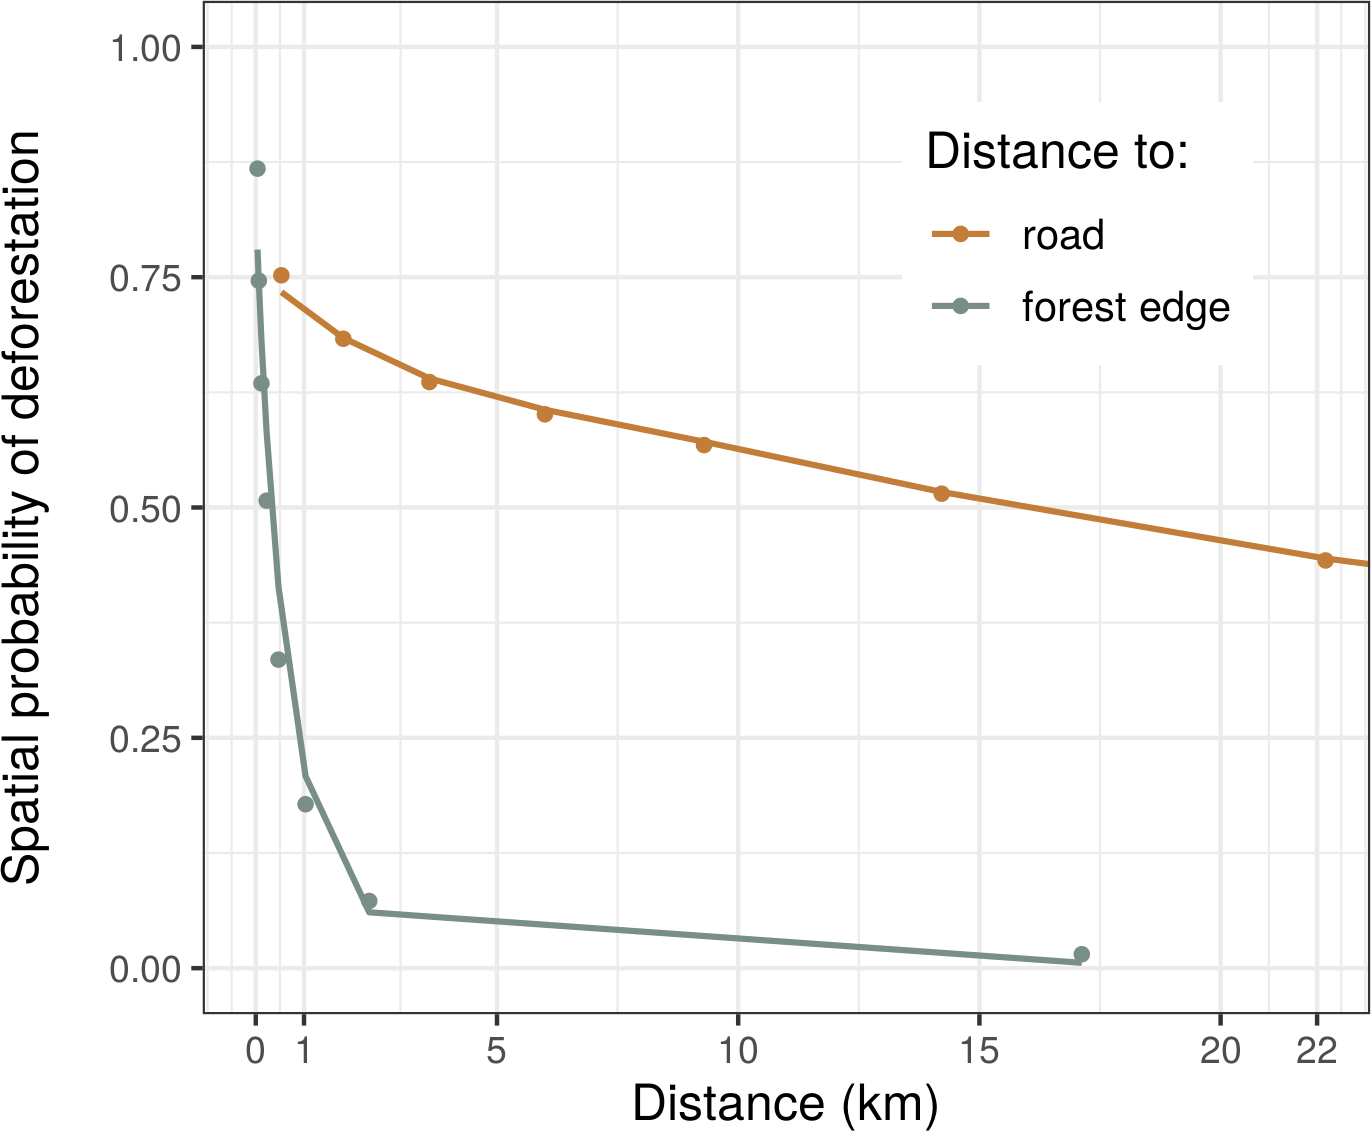
\includegraphics[width=\textwidth]{figs/article/proba-roads}

\textbf{Effects of roads and forest edge on the deforestation risk}
\end{column}
\end{columns}
\end{frame}

\section{Discussion}
\label{sec:org3132b2c}
\subsection{Uncertainty analysis}
\label{sec:orga11198d}
\begin{frame}[label={sec:orgf0e44a4}]{Uncertainty analysis}
\begin{itemize}
\item Despite uncertainty, results are clear and alarming.
\item ``Business-as-usual'' scenario \(\neq\) what \textbf{will} happen in the
future.
\item ``Business-as-usual'' scenario \(=\) in the absence of any change.
\item The objective is to alert and create a momentum for change.
\item Nonetheless, rather optimistic scenario.
\end{itemize}

\vspace{0.25cm}
\centering 
\includegraphics[width=0.6\textwidth]{figs/madame-irma}
\end{frame}

\subsection{Alternative scenarios}
\label{sec:orgce54724}
\begin{frame}[label={sec:org320016d}]{Alternative scenarios: demography and demand}
\begin{itemize}
\item Demography: in Africa, a large part of the population depends on
slash-and-burn agriculture for their livelihood.
\item Increasing demand for agricultural commodities: e.g., palm oil, Corley
et al. 2009
\end{itemize}

\vspace{0.25cm}
\centering 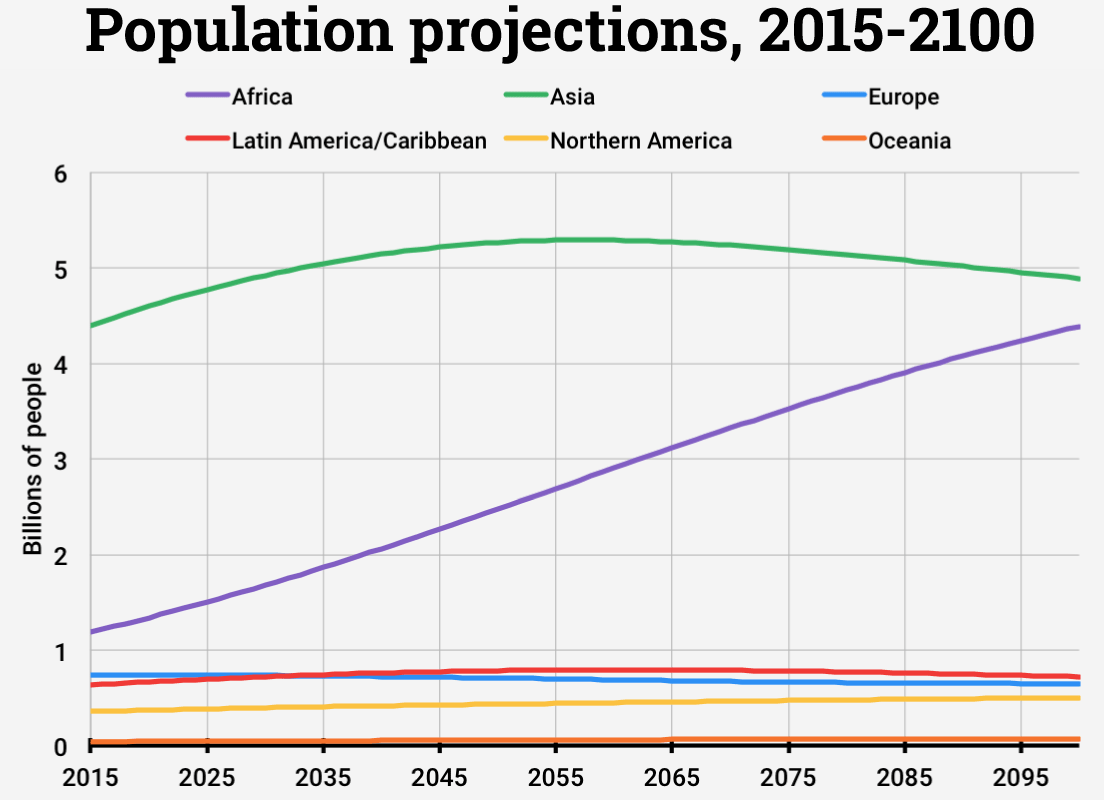
\includegraphics[width=0.45\textwidth]{figs/UN-regional-pop-projections}
\centering 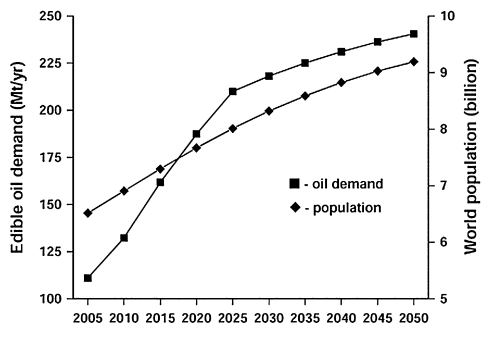
\includegraphics[width=0.45\textwidth]{figs/oil-palm-proj}
\end{frame}

\subsection{Other perspectives}
\label{sec:org4e664b5}
\begin{frame}[label={sec:orge4cec1e}]{Other perspectives}
\begin{itemize}
\item Models can be refined locally (e.g., Ivory-Coast, Madagascar,
New-Caledonia) with more information on the context.
\item Very rough estimates of biodiversity loss: need for world biodiversity
maps.
\item (Fragmentation study, regeneration potential, etc.)
\end{itemize}

\vspace{0.25cm}
\centering 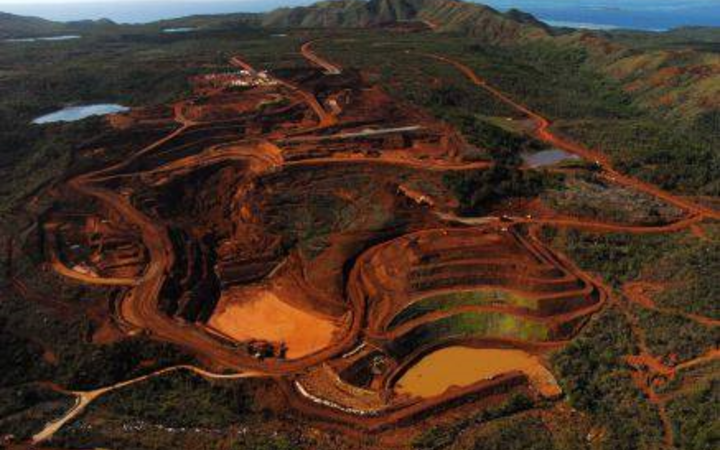
\includegraphics[width=0.6\textwidth]{figs/mines-NC}

\textbf{Mining activity in New-Caledonia}
\end{frame}

% %%%%%%%%%%%%%%%%%%%%%%%%%%%%%%%%%%%%%%%%%%%%%%%%%%%%%%%%%%

{
  % Use background image
  \usebackgroundtemplate{%
    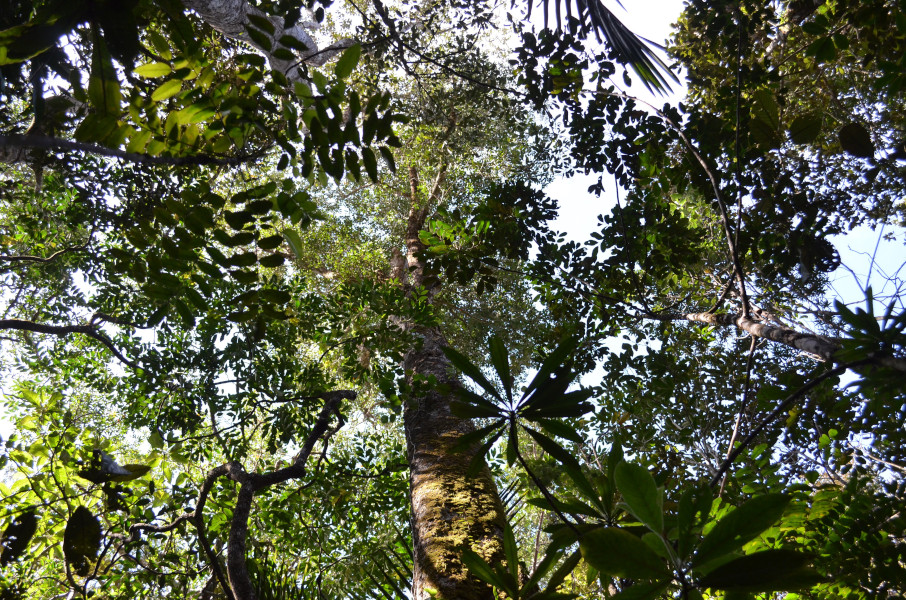
\includegraphics[keepaspectratio=true, height=\paperheight]{figs/Canopy-NC}
  }
  \setbeamertemplate{navigation symbols}{}
  % Remove shadow from block
  \setbeamertemplate{blocks}[rounded][shadow=false]
  \begin{frame}[plain]
  	\vspace*{\stretch{100}} 
    \begin{block}{}
      \begin{center}
        \ldots~Thank you for attention~\ldots \\
        \url{https://forestatrisk.cirad.fr} \\
        
\includegraphics[width=0.8\textwidth]{figs/partners_logos}
      \end{center}
    \end{block}
  \end{frame}
}
\end{document}
